\documentclass{article}
\usepackage{hyperref}       % hyperlinks
\usepackage{url}      
% simple URL typesetting
\usepackage{booktabs}       % professional-quality tables
\usepackage{amsfonts}       % blackboard math symbols
\usepackage{amssymb}
\usepackage{nicefrac}    
\usepackage[numbers,sort]{natbib}
% compact symbols for 1/2, etc.
\usepackage{microtype}      % microtypography
\usepackage{xcolor}      
%%%%%%%%%%%---SETME-----%%%%%%%%%%%%%
%replace @@ with the submission number submission site.
\newcommand{\thiswork}{INF$^2$\xspace}
%%%%%%%%%%%%%%%%%%%%%%%%%%%%%%%%%%%%


%\newcommand{\rev}[1]{{\color{olivegreen}#1}}
\newcommand{\rev}[1]{{#1}}


\newcommand{\JL}[1]{{\color{cyan}[\textbf{\sc JLee}: \textit{#1}]}}
\newcommand{\JW}[1]{{\color{orange}[\textbf{\sc JJung}: \textit{#1}]}}
\newcommand{\JY}[1]{{\color{blue(ncs)}[\textbf{\sc JSong}: \textit{#1}]}}
\newcommand{\HS}[1]{{\color{magenta}[\textbf{\sc HJang}: \textit{#1}]}}
\newcommand{\CS}[1]{{\color{navy}[\textbf{\sc CShin}: \textit{#1}]}}
\newcommand{\SN}[1]{{\color{olive}[\textbf{\sc SNoh}: \textit{#1}]}}

%\def\final{}   % uncomment this for the submission version
\ifdefined\final
\renewcommand{\JL}[1]{}
\renewcommand{\JW}[1]{}
\renewcommand{\JY}[1]{}
\renewcommand{\HS}[1]{}
\renewcommand{\CS}[1]{}
\renewcommand{\SN}[1]{}
\fi

%%% Notion for baseline approaches %%% 
\newcommand{\baseline}{offloading-based batched inference\xspace}
\newcommand{\Baseline}{Offloading-based batched inference\xspace}


\newcommand{\ans}{attention-near storage\xspace}
\newcommand{\Ans}{Attention-near storage\xspace}
\newcommand{\ANS}{Attention-Near Storage\xspace}

\newcommand{\wb}{delayed KV cache writeback\xspace}
\newcommand{\Wb}{Delayed KV cache writeback\xspace}
\newcommand{\WB}{Delayed KV Cache Writeback\xspace}

\newcommand{\xcache}{X-cache\xspace}
\newcommand{\XCACHE}{X-Cache\xspace}


%%% Notions for our methods %%%
\newcommand{\schemea}{\textbf{Expanding supported maximum sequence length with optimized performance}\xspace}
\newcommand{\Schemea}{\textbf{Expanding supported maximum sequence length with optimized performance}\xspace}

\newcommand{\schemeb}{\textbf{Optimizing the storage device performance}\xspace}
\newcommand{\Schemeb}{\textbf{Optimizing the storage device performance}\xspace}

\newcommand{\schemec}{\textbf{Orthogonally supporting Compression Techniques}\xspace}
\newcommand{\Schemec}{\textbf{Orthogonally supporting Compression Techniques}\xspace}



% Circular numbers
\usepackage{tikz}
\newcommand*\circled[1]{\tikz[baseline=(char.base)]{
            \node[shape=circle,draw,inner sep=0.4pt] (char) {#1};}}

\newcommand*\bcircled[1]{\tikz[baseline=(char.base)]{
            \node[shape=circle,draw,inner sep=0.4pt, fill=black, text=white] (char) {#1};}}
\usepackage[a4paper, margin=1in]{geometry}

\usepackage[ruled]{algorithm2e} % For algorithms


%% ADDED BY KRISHNA for subcaption
\let\subfigure\relax
\usepackage{subcaption}
\usepackage{graphicx}
\usepackage{caption}
\usepackage{subcaption}
\newcommand{\norm}[1]{\left\| #1 \right\|}

%% END ADDED BY KRISHNA 
\renewcommand{\algorithmcfname}{ALGORITHM}
\SetAlFnt{\small}
\SetAlCapFnt{\small}
\SetAlCapNameFnt{\small}
\SetAlCapHSkip{0pt}
\IncMargin{-\parindent}



% FOR COMMENTS

\newcommand{\juba}[1]{\textcolor{red}{[Juba: #1]}}
\newcommand{\vidya}[1]{\textcolor{red}{[Vidya: #1]}}
\newcommand{\gua}[1]{\textcolor{green}{[Guanghui: #1]}}
\newcommand{\kri}[1]{\textcolor{blue}{[Krishna: #1]}}

\renewcommand{\juba}[1]{}
 \renewcommand{\vidya}[1]{}
 \renewcommand{\gua}[1]{}
 \renewcommand{\kri}[1]{}
% FOR COMMENTS


\begin{document}


\begin{center}

{\bf{\Large{Multi-Agent Performative Prediction Beyond the Insensitivity Assumption: A Case Study for Mortgage Competition}}}

\vspace*{.2in}



{\large{
\begin{tabular}{cccc}
 Guanghui Wang$^1$, Krishna Acharya$^2$, Lokranjan Lakshmikanthan$^2$\\
 Vidya Muthukumar$^{2,3}$, Juba Ziani$^{2}$  \\
\end{tabular}}}

\vspace*{.05in}

\begin{tabular}{c}
$^1$College of Computing, Georgia Institute of Technology\\
$^2$School of Industrial and Systems Engineering, Georgia Institute of Technology\\
$^3$School of Electrical and Computer Engineering, Georgia Institute of Technology\\
  \texttt{\{gwang369,krishna.acharya,llakshmi3,vmuthukumar8,jziani3\}@gatech.edu}
\end{tabular}

\vspace*{.2in}
\date{}

\end{center}


% FOR COMMENTS

\begin{abstract}
Performative prediction models account for feedback loops in decision-making processes where predictions influence future data distributions. While existing work largely assumes insensitivity of data distributions to small strategy changes, this assumption usually fails in real-world competitive (i.e. multi-agent) settings. For example, in Bertrand-type competitions, a small reduction in one firm's price can lead that firm to capture the entire demand, while all others sharply lose all of their customers. 

We study a representative setting of multi-agent performative prediction in which insensitivity assumptions do not hold, and investigate the convergence of natural dynamics. To do so, we focus on a specific game that we call the ``Bank Game'', where two lenders compete over interest rates and credit score thresholds. Consumers act similarly as to in a Bertrand Competition, with each consumer selecting the firm with the lowest interest rate \emph{that they are eligible for based on the firms' credit thresholds}. Our analysis characterizes the equilibria of this game and demonstrates that when both firms use a common and natural no-regret learning dynamic---exponential weights---with proper initialization, the dynamics \emph{always} converge to stable outcomes despite the general-sum structure. Notably, our setting admits multiple stable equilibria, with convergence dependent on initial conditions. We also provide theoretical convergence results in the stochastic case when the utility matrix is not fully known, but each learner can observe sufficiently many samples of consumers at each time step to estimate it, showing robustness to slight mis-specifications. Finally, we provide experimental results that validate our theoretical findings.
\end{abstract}

\section{Introduction}
%\textcolor{red}{draft that lays out the mian story but needs some rewriting and a pass for clarity for a non-expert reader}
\section{Introduction}


\begin{figure}[t]
\centering
\includegraphics[width=0.6\columnwidth]{figures/evaluation_desiderata_V5.pdf}
\vspace{-0.5cm}
\caption{\systemName is a platform for conducting realistic evaluations of code LLMs, collecting human preferences of coding models with real users, real tasks, and in realistic environments, aimed at addressing the limitations of existing evaluations.
}
\label{fig:motivation}
\end{figure}

\begin{figure*}[t]
\centering
\includegraphics[width=\textwidth]{figures/system_design_v2.png}
\caption{We introduce \systemName, a VSCode extension to collect human preferences of code directly in a developer's IDE. \systemName enables developers to use code completions from various models. The system comprises a) the interface in the user's IDE which presents paired completions to users (left), b) a sampling strategy that picks model pairs to reduce latency (right, top), and c) a prompting scheme that allows diverse LLMs to perform code completions with high fidelity.
Users can select between the top completion (green box) using \texttt{tab} or the bottom completion (blue box) using \texttt{shift+tab}.}
\label{fig:overview}
\end{figure*}

As model capabilities improve, large language models (LLMs) are increasingly integrated into user environments and workflows.
For example, software developers code with AI in integrated developer environments (IDEs)~\citep{peng2023impact}, doctors rely on notes generated through ambient listening~\citep{oberst2024science}, and lawyers consider case evidence identified by electronic discovery systems~\citep{yang2024beyond}.
Increasing deployment of models in productivity tools demands evaluation that more closely reflects real-world circumstances~\citep{hutchinson2022evaluation, saxon2024benchmarks, kapoor2024ai}.
While newer benchmarks and live platforms incorporate human feedback to capture real-world usage, they almost exclusively focus on evaluating LLMs in chat conversations~\citep{zheng2023judging,dubois2023alpacafarm,chiang2024chatbot, kirk2024the}.
Model evaluation must move beyond chat-based interactions and into specialized user environments.



 

In this work, we focus on evaluating LLM-based coding assistants. 
Despite the popularity of these tools---millions of developers use Github Copilot~\citep{Copilot}---existing
evaluations of the coding capabilities of new models exhibit multiple limitations (Figure~\ref{fig:motivation}, bottom).
Traditional ML benchmarks evaluate LLM capabilities by measuring how well a model can complete static, interview-style coding tasks~\citep{chen2021evaluating,austin2021program,jain2024livecodebench, white2024livebench} and lack \emph{real users}. 
User studies recruit real users to evaluate the effectiveness of LLMs as coding assistants, but are often limited to simple programming tasks as opposed to \emph{real tasks}~\citep{vaithilingam2022expectation,ross2023programmer, mozannar2024realhumaneval}.
Recent efforts to collect human feedback such as Chatbot Arena~\citep{chiang2024chatbot} are still removed from a \emph{realistic environment}, resulting in users and data that deviate from typical software development processes.
We introduce \systemName to address these limitations (Figure~\ref{fig:motivation}, top), and we describe our three main contributions below.


\textbf{We deploy \systemName in-the-wild to collect human preferences on code.} 
\systemName is a Visual Studio Code extension, collecting preferences directly in a developer's IDE within their actual workflow (Figure~\ref{fig:overview}).
\systemName provides developers with code completions, akin to the type of support provided by Github Copilot~\citep{Copilot}. 
Over the past 3 months, \systemName has served over~\completions suggestions from 10 state-of-the-art LLMs, 
gathering \sampleCount~votes from \userCount~users.
To collect user preferences,
\systemName presents a novel interface that shows users paired code completions from two different LLMs, which are determined based on a sampling strategy that aims to 
mitigate latency while preserving coverage across model comparisons.
Additionally, we devise a prompting scheme that allows a diverse set of models to perform code completions with high fidelity.
See Section~\ref{sec:system} and Section~\ref{sec:deployment} for details about system design and deployment respectively.



\textbf{We construct a leaderboard of user preferences and find notable differences from existing static benchmarks and human preference leaderboards.}
In general, we observe that smaller models seem to overperform in static benchmarks compared to our leaderboard, while performance among larger models is mixed (Section~\ref{sec:leaderboard_calculation}).
We attribute these differences to the fact that \systemName is exposed to users and tasks that differ drastically from code evaluations in the past. 
Our data spans 103 programming languages and 24 natural languages as well as a variety of real-world applications and code structures, while static benchmarks tend to focus on a specific programming and natural language and task (e.g. coding competition problems).
Additionally, while all of \systemName interactions contain code contexts and the majority involve infilling tasks, a much smaller fraction of Chatbot Arena's coding tasks contain code context, with infilling tasks appearing even more rarely. 
We analyze our data in depth in Section~\ref{subsec:comparison}.



\textbf{We derive new insights into user preferences of code by analyzing \systemName's diverse and distinct data distribution.}
We compare user preferences across different stratifications of input data (e.g., common versus rare languages) and observe which affect observed preferences most (Section~\ref{sec:analysis}).
For example, while user preferences stay relatively consistent across various programming languages, they differ drastically between different task categories (e.g. frontend/backend versus algorithm design).
We also observe variations in user preference due to different features related to code structure 
(e.g., context length and completion patterns).
We open-source \systemName and release a curated subset of code contexts.
Altogether, our results highlight the necessity of model evaluation in realistic and domain-specific settings.






\section{Model}\label{sec1}
\section{Model}
\label{sec:model}
Let $[N] = \{1, 2, \dots, N \}$ be a set of $N$ agents.
We examine an environment in which a system interacts with the agents over $T$ rounds.
Every round $t\leq T$ comprises $N$ \emph{sessions}, each session represents an encounter of the system with exactly one agent, and each agent interacts exactly once with the system every round.
I.e., in each round $t$ the agents arrive sequentially. 


\paragraph{Arrival order} The \emph{arrival order} of round $t$, denoted as $\ordv_t=(\ord_t(1),\dots, \ord_t(N))$, is an element from set of all permutations of $[N]$. Each entry $q$ in $\ordv_t$ is the index of the agent that arrives in the $q^{\text{th}}$ session of round $t$.
For example, if $\ord_t(1) = 2$, then agent $2$ arrives in the first session of round $t$.
Correspondingly, $\ord_t^{-1}(i)=q$ implies that agent $i$ arrives in the $q^{\text{th}}$ session of round $t$. 

As we demonstrate later, the arrival order has an immediate impact on agent rewards. We call the mechanism by which the arrival order is set \emph{arrival function} and denote it by $\ordname$. Throughout the paper, we consider several arrival functions such as the \emph{uniform arrival} function, denoted by $\uniord$, and the \emph{nudged arrival} $\sugord$; we introduce those formally in Sections~\ref{sec:uniform} and~\ref{sec:nudge}, respectively.

%We elaborate more on this concept in Section~\ref{sec: arrival}.


\paragraph{Arms} We consider a set of $K \geq 2$ arms, $A = \{a_1, \ldots, a_K\}$. The reward of arm $a_i$ in round $t$ is a random variable $X_i^t \sim \mathcal{D}^t_i$, where the rewards $(X_i^t)_{i,t}$ are mutually independent and bounded within the interval $[0,1]$. The reward distribution $\mathcal{D}^t_i$ of arm $a_i$, $i\in [K]$ at round $t\in T$ is assumed to be non-stationary but independent across arms and rounds. We denote the realized reward of arm $a_i$ in round $t$ by $x_i^t$. We assume \emph{reward consistency}, meaning that rewards may vary between rounds but remain constant within the sessions of a single round. Specifically, if an arm $a_i$ is selected multiple times during round~$t$, each selection yields the same reward $x_i^t$, where the superscript $t$ indicates its dependence on the round rather than the session. This consistency enables the system to leverage information obtained from earlier sessions to make more informed decisions in later sessions within the same round. We provide further details on this principle in Subsection~\ref{subsec:information}.


\paragraph{Algorithms} An algorithm is a mapping from histories to actions. We typically expect algorithms to maximize some aggregated agent metric like social welfare. Let $\mathcal H^{t,q}$ denote the information observed during all sessions of rounds $1$ to $t-1$ and sessions $1$ to $q-1$ in round $t$.  The history $\mathcal H^{t,q}$ is an element from $(A \times [0,1])^{(t-1) \cdot N +q-1}$, consisting of pairs of the form (pulled arm, realized reward). Notice that we restrict our attention to \emph{anonymous} algorithms, i.e., algorithms that do not distinguish between agents based on their identities. Instead, they only respond to the history of arms pulled and rewards observed, without conditioning on which specific agent performed each action.
%In the most general case, algorithms make decisions at session $q$ of round $t$  based on the entire history $\mathcal H^{t,q}$ and the index of the arriving agent $\ord_t(q)$. %Furthermore, we sometimes assume that algorithms have Bayesian information, i.e., algorithms are aware of the distributions $(\mathcal D_i)^K_{i=1}$. 
Furthermore, we sometimes assume that algorithms have Bayesian information, meaning they are aware of the reward distributions $(\mathcal{D}^t_i)_{i,t}$. If such an assumption is required to derive a result, we make it explicit. %Otherwise, we do not assume any additional knowledge about the algorithm’s information. %This distinction allows us to analyze both general algorithms without prior distributional knowledge and specialized algorithms that leverage Bayesian information.


\paragraph{Rewards} Let $\rt{i}$ denote the reward received by agent $i \in [N]$ at round $t$, and let $\Rt{i}$ denote her cumulative reward at the end of round $t$, i.e., $\Rt{i} = \sum_{\tau=1}^{t}{r^{\tau}_{i}}$. We further denote the \emph{social welfare} as the sum of the rewards all agents receive after $T$ rounds. Formally, $\sw=\sum^{N}_{i=1}{R^T_i}$. We emphasize that social welfare is independent of the arrival order. 


\paragraph{Envy}
We denote by $\adift{i}{j}$ the reward discrepancy of agents $i$ and $j$ in round $t$; namely, $\adift{i}{j}= \rt{i} - \rt{j}$. %We call this term \omer{name??} reward discrepancy in round $t$. 
The (cumulative) \emph{envy} between two agents at round $t$ is the difference in their cumulative rewards. Formally, $\env_{i,j}^t= \Rt{i} - \Rt{j}$ is the envy after $t$ rounds between agent $i$ and $j$. We can also formulate envy as the sum of reward discrepancies, $\env_{i,j}^t= \sum^{t}_{\tau=1}{\adif{i}{j}^\tau}$. Notice that envy is a signed quantity and can be either positive or negative. Specifically, if $\env_{i,j}^t < 0$, we say that agent $i$ envies agent $j$, and if $\env_{i,j}^t > 0$, agent $j$ envies agent $i$. The main goal of this paper is to investigate the behavior of the \emph{maximal envy}, defined as
\[
\env^t = \max_{i,j \in [N]} \env^t_{i,j}.
\]
For clarity, the term \emph{envy} will refer to the maximal envy.\footnote{ We address alternative definitions of envy in Section~\ref{sec:discussion}.} % Envy can also be defined in alternative ways, such as by averaging pairwise envy across all agents. We address average envy in Section~\ref{sec:avg_envy}.}
Note that $\env_{i,j}^t$ are random variables that depend on the decision-making algorithm, realized rewards, and the arrival order, and therefore, so is $\env^t$. If a result we obtain regarding envy depends on the arrival order $\ordname$, we write $\env^t(\ordname)$. Similarly, to ease notation, if $\ordname$ can be understood from the context, it is omitted.



\paragraph{Further Notation} We use the subscript $(q)$ to address elements of the $q^{\text{th}}$ session, for $q\in [N]$.
That is, we use the notation $\rt{(q)}$ to denote the reward granted to the agent that arrives in the $q^{\text{th}}$ session of round $t$ and $\Rt{(q)}$ to denote her cumulative reward. %Additionally, we introduce the notation $\at{(q)}$ to denote the arm pulled in that session.
Correspondingly, $\sdift{q}{w} = \rt{(q)} - \rt{(w)}$ is the reward discrepancy of the agents arriving in the $q^{\text{th}}$ and $w^{\text{th}}$ sessions of round $t$, respectively. 
To distinguish agents, arms, sessions and rounds, we use the letters $i,j$ to mark agents and arms, $q,w$ for sessions, and $t,\tau$ for rounds.


\subsection{Example}
\label{sec: example}
To illustrate the proposed setting and notation, we present the following example, which serves as a running example throughout the paper.

\begin{table}[t]
\centering
\begin{tabular}{|c|c|c|c|}
\hline
$t$ (round) & $\ordv_t$ (arrival order) & $x_1^t$ & $x_2^t$ \\ \hline
1           & 2, 1                     & 0.6     & 0.92    \\ \hline
2           & 1, 2                     & 0.48    & 0.1     \\ \hline
3           & 2, 1                     & 0.15    & 0.8     \\ \hline
\end{tabular}
\caption{
    Data for Example~\ref{example 1}.
}
\label{tbl: example}
\end{table}

\begin{algorithm}[t]
\caption{Algorithm for Example~\ref{example 1}}
\label{alguni}
\DontPrintSemicolon 
\For{round $t = 1$ to $T$}{
    pull $a_{1}$ in the first session\label{alguniexample: first}\\
    \lIf{$x^t_1 \geq \frac{1}{2}$}{pull $a_{1}$ again in second session \label{alguniexample: pulling a again}}
    \lElse{pull $a_{2}$ in second session \label{alguniexample: sopt else}}
}
\end{algorithm}


\begin{example}\label{example 1}
We consider $K=2$ uniform arms, $X_1,X_2 \sim \uni{0,1}$, and $N=2$ for some $T\geq 3$. We shall assume arm decision are made by Algorithm~\ref{alguni}: In the first session, the algorithm pulls $a_1$; if it yields a reward greater than $\nicefrac{1}{2}$, the algorithm pulls it again in the second session (the ``if'' clause). Otherwise, it pulls $a_2$.



We further assume that the arrival orders and rewards are as specified in Table~\ref{tbl: example}. Specifically, agent 2 arrives in the first session of round $t=1$, and pulling arm $a_2$ in this round would yield a reward of $x^1_2 = 0.92$. Importantly, \emph{this information is not available to the decision-making algorithm in advance} and is only revealed when or if the corresponding arms are pulled.




In the first round, $\boldsymbol{\eta}^1 = \left(2,1\right)$; thus, agent 2 arrives in the first session.
The algorithm pulls arm $a_1$, which means, $a^1_{(1)} = a_1$, and the agent receives $r_{2}^1=r_{(1)}^1=x_1^1=0.6$.
Later that round, in the second session, agent 1 arrives, and the algorithm pulls the same arm again since $x^1_1 = 0.6 \geq \nicefrac{1}{2}$ due to the ``if'' clause.
I.e., $a^1_{(2)} = a_1$ and $r_{1}^1 = r_{(2)}^1 = x_1^1 = 0.6$.
Even though the realized reward of arm $a_2$ in that round is higher ($0.92$), the algorithm is not aware of that value.
At the end of the first round, $R^1_1 = R^1_{(2)} = R^1_2 = R^1_{(1)} = 0.6$. The reward discrepancy is thus $\adif{1}{2}^1 = \adif{2}{1}^1= \sdif{2}{1}^1 = 0.6 - 0.6 =0$. 



In the second round, agent 1 arrives first, followed by agent 2.
Firstly, the algorithm pulls arm $a_1$ and agent 1 receives a reward of $r_{1}^2 = r_{(1)}^2 = x_1^2 = 0.48$.
Because the reward is lower than $\nicefrac{1}{2}$, in the second session the algorithm pulls the other arm ($a^2_{(2)} = a_2$), granting agent 2 a reward of $r_{2}^2 = r_{(2)}^2 = x_2^2 = 0.1$.
At the end of the second round, $R^2_1 = R^2_{(1)} = 0.6 + 0.48 = 1.08$ and $R^2_2 = R^2_{(2)} = 0.6 + 0.1 = 0.7$. Furthermore, $\sdif{2}{1}^2 = \adif{2}{1}^2 = r^2_{2} - r^2_{1} = 0.1 - 0.48 = -0.38$.

In the third and final round, agent 2 arrives first again, and receives a reward  of $0.15$ from $a_1$. When agent 1 arrives in the second session, the algorithm pulls arm $a_2$, and she receives a reward of $0.8$. As for the reward discrepancy, $\sdif{2}{1}^3 = \adif{2}{1}^3 = r^3_{2} - r^3_{1} = 0.15 - 0.8 = -0.75$. 

Finally, agent 1 has a cumulative reward of $R^3_1 = R^3_{(2)} = 0.6 + 0.48 + 0.8 = 1.88$, whereas agent~2 has a cumulative reward of $R^3_2 = R^3_{(1)} = 0.6 + 0.1 + 0.15 = 0.85$. In terms of envy, $\env^1_{1,2}= \adif{1}{2}^1 =0$, $\env^2_{1,2}=\adif{1}{2}^1+\adif{1}{2}^2= 0.38$, and $\env^3_{1,2} = -\env^3_{2,1} = R^3_1-R^3_2 = 1.88-0.85 = 1.03$, and consequently the envy in round 3 is $\env^3 = 1.03$.
\end{example}


\subsection{Information Exploitation}
\label{subsec:information}

In this subsection, we explain how algorithms can exploit intra-round information.
Since rewards are consistent in the sessions of each round, acquiring information in each session can be used to increase the reward of the following sessions.
In other words, the earlier sessions can be used for exploration, and we generally expect agents arriving in later sessions to receive higher rewards.
Taken to the extreme, an agent that arrives after all arms have been pulled could potentially obtain the highest reward of that round, depending on how the algorithm operates.

To further demonstrate the advantage of late arrival, we reconsider Example~\ref{example 1} and Algorithm~\ref{alguni}. 
The expected reward for the agent in the first session of round $t$ is $\E{\rt{(1)}}=\mu_1=\frac{1}{2}$, yet the expected reward of the agent in the second session is
\begin{align*}
\E{\rt{(2)}}=\E{\rt{(2)}\mid X^t_1 \geq \frac{1}{2} }\prb{X^t_1 \geq \frac{1}{2}} + \E{\rt{(2)}\mid X^t_1 < \frac{1}{2} }\prb{X^t_1 < \frac{1}{2}};
\end{align*}
thus, $\E{\rt{(2)}} =\E{X^t_1\mid X^t_1 \geq \frac{1}{2} }\cdot \frac{1}{2} + \mu_2\cdot\frac{1}{2} = \frac{5}{8}$.
Consequently, the expected welfare per round is $\E{\rt{(1)}+\rt{(2)}}=1+\frac{1}{8}$, and the benefit of arriving in the second session of any round $t$ is $\E{\rt{(2)} - \rt{(1)}} = \frac{1}{8}$. This gap creates envy over time, which we aim to measure and understand.
%This discrepancy generates envy over time, and our paper aims to better understand it.
\subsection{Socially Optimal Algorithms}
\label{sec: sw}
Since our model is novel, particularly in its focus on the reward consistency element, studying social welfare maximizing algorithms represents an important extension of our work. While the primary focus of this paper is to analyze envy under minimal assumptions about algorithmic operations, we also make progress in the direction of social welfare optimization. See more details in Section~\ref{sec:discussion}.%Due to space limitations, we defer the discussion on socially optimal algorithms to  \ifnum\Includeappendix=0{the appendix}\else{Section~\ref{appendix:sociallyopt}}\fi.




% Since our model is novel and specifically the reward consistency element, it might be interesting to study social welfare optimization. While the main focus of our paper is to study envy under minimal assumptions on how the algorithm operates, we take steps toward this direction as well. Due to space limitations, we defer the discussion on socially optimal algorithms to  \ifnum\Includeappendix=0{the appendix}\else{Section~\ref{appendix:sociallyopt}}\fi.  We devise a socially optimal algorithm for the two-agent case, offer efficient and optimal algorithms for special cases of $N>2$ agents, and an inefficient and approximately optimal algorithm for any instance with $N>2$. Moreover, we address the welfare-envy tradeoff in Section~\ref{sec:extensions}.


% Social welfare, unlike envy, is entirely independent of the arrival order. While the main focus of our paper is to study envy under minimal assumptions on how the algorithm operates, socially optimal algorithms might also be of interest. Due to space limitations, we defer the discussion on socially optimal algorithms to  \ifnum\Includeappendix=0{the appendix}\else{Section~\ref{appendix:sociallyopt}}\fi. We devise a socially optimal algorithm for the two-agent case, offer efficient and optimal algorithms for special cases of $N>2$ agents, and an inefficient and approximately optimal algorithm for any instance with $N>2$. %Furthermore, we treat the welfare-envy tradeoff of the special case of Example~\ref{example 1}.




\section{Equilibria of the One-Shot Game under Two Discrete Actions}
\label{sec:understand NE}
In this section, we introduce the equilibrium concepts that we use for solving the static, one-shot version of our game. We then fully characterize the equilibria of our problem. 

\subsection{Equilibrium Concepts}

We start by defining the main solution concepts used in this section, in the \emph{one-shot} setting. The main solution concept used in this paper is the concept of \emph{Nash equilibrium}: 

\begin{definition}[Nash equilibrium]
A pair of strategies \((\theta_1^*, \theta_2^*)\) constitutes a \emph{pure Nash equilibrium} (pure NE) iff:
\[
u_1(\theta_1^*, \theta_2^*) \geq \max_{\theta_1\in \Gamma\times \Lambda} u_1(\theta_1, \theta_2^*), \quad \text{and} \quad u_2(\theta_1^*, \theta_2^*) \geq \max_{\theta_2\in \Gamma\times \Lambda} u_2(\theta_1^*, \theta_2).
\]
\noindent A pair of mixed strategies \((p_1^*, p_2^*)\) constitutes a \emph{mixed Nash equilibrium} (mixed NE) if and only if the following conditions hold:  
\[
\E_{\theta_1 \sim p_1^*, \theta_2 \sim p_2^*}[u_1(\theta_1, \theta_2)] \geq \max_{p \in \Delta(\Gamma \times \Lambda)} \E_{\theta_1 \sim p, \theta_2 \sim p_2^*}[u_1(\theta_1, \theta_2)],
\]
and  
\[
\E_{\theta_1 \sim p_1^*, \theta_2 \sim p_2^*}[u_2(\theta_1, \theta_2)] \geq \max_{p \in \Delta(\Gamma \times \Lambda)} \E_{\theta_1 \sim p_1^*, \theta_2 \sim p}[u_2(\theta_1, \theta_2)].
\]
\end{definition}

In Nash equilibria, players pick their actions simultaneously and independently of each other. Beyond Nash Equilibria, we also consider the concept of Correlated Equilibria (CEs) of a game, where coordination among players is allowed: 

\begin{definition}[Correlated Equilibrium (CE)] 
\label{defn:CE}
A joint probability distribution $p$ \text{over} pairs of strategies $(\theta_1,\theta_2) \in \Theta_1 \times \Theta_2$ is a correlated equilibrium if, for each $i \in \{1,2\}$,
\[
\sum_{\theta_{2} \in \Theta_{2}} p(\theta_1,\theta_2)\, u_1(\theta_1,\theta_2)
\geq 
\sum_{\theta_2 \in \Theta_2} p(\theta_1,\theta_2)\, u_1(\theta'_1,\theta_2),
~~\forall \theta_1,\theta'_1 \in \Theta_1,
\]
and 
\[
\sum_{\theta_{1} \in \Theta_{1}} p(\theta_1,\theta_2)\, u_2(\theta_1,\theta_2)
\geq 
\sum_{\theta_1 \in \Theta_1} p(\theta_1,\theta_2)\, u_2(\theta_1,\theta'_2),
~~\forall \theta_2,\theta'_2 \in \Theta_2.
\]
\end{definition}

Informally, correlated equilibria use a correlation or signaling device that recommend an action $(\theta_1,\theta_2)$ to the players according to a \emph{joint} distribution (for example, think of a traffic signal at an intersection). At a correlated equilibrium, no player benefits from deviating from the recommended action in expectation.  
%{\color{red} Vidya: I think some of this is maybe removable, especially since we ultimately do not have real results for CE beyond the one-shot characterization} \gua{I added some discussion under the CE theorem. }


\subsection{One-Shot Equilibrium Characterization for $n=2$ Actions} 

To simplify presentation, we introduce the following function, which is useful in writing down players' utilities: 
%which is essentially the utility under $D_y$ for a particular bank as a function of its interest rate $\gamma$, threshold $\tau$ and threshold range $[\tau_a, \tau_b]$ (recall that the threshold range is determined in part by the bank's own choice of threshold $\tau$ but also the strategy of the competing bank, if it exists).
% {\color{red} Is it always true that $\tau_a = \tau$? Is it ever possible for $\tau_b < \tau_a$, meaning that the bank would never attract customers?}
% Then, if $\tau_a<\tau_b$, the utility of the bank is given by:
\begin{equation}
\label{eqn:utility-onebank}
    f_{D_y}(\gamma,\tau_a,\tau_b)
    \triangleq
    \int_{\tau_a}^{\tau_b}[(2+\gamma)y-1]p(y)dy.
\end{equation}
We often omit the subscript $D_y$ when it is clear from context. Intuitively, this represents the utility for a single bank who sets the interest rate as $\gamma$ and is able to attract all the customers in the range $Y \in [\tau_a,\tau_b]$. %\gua{I added this sentence}

As discussed in Section \ref{sec1}, we focus on the simplest case where there are two choices for each parameter: \(0 \leq \tau_{\ell} < \tau_{h} \leq 1\) and \(0 \leq \gamma_{\ell} < \gamma_{h} \leq 1\). In this scenario, the utility of Bank 1 under each pair of decisions forms a \(4 \times 4\) matrix (as shown in Table \ref{tab:my-table}). We consider the canonical case where:
\[
\tau_{\ell} = \frac{1}{2 + \gamma_{h}}, \quad \text{and} \quad \tau_{h} = \frac{1}{2 + \gamma_{\ell}}.
\]

These choices for the thresholds are natural from Equation~\eqref{eqn:utility-onebank}. Indeed, it is a dominant strategy for a \emph{rational} bank with interest rate $\gamma$ to set a threshold of $\tau^*(\gamma) := \frac{1}{ 2 + \gamma}$. Setting a higher threshold $\tau > \tau^*(\gamma)$ leads to ignoring customers in the range $y \in [\tau^*(\gamma), \tau]$ that provide a utility of $(2 + \gamma) y - 1 > 0$, while setting a lower threshold $\tau < \tau^*(\gamma)$ leads to potentially incorporating some customers in the range $y < \tau^*(\gamma)$ that would yield a utility of $(2 + \gamma) y - 1 < 0$ as a result of low probability of repayment; both cases cannot improve total utility.
%{\color{red} I think the originally written discussion of threshold range $[\tau_a,\tau_b]$ was quite confusing. I have taken a shot at revising it}



\begin{table}[!h]
\centering
\begin{tabular}{@{}ccccc@{}}
\toprule
\textbf{} &
  \textbf{$(\tau_{\ell},\gamma_{\ell})$} &
  \textbf{$(\tau_{\ell},\gamma_{h})$} &
  $(\tau_{h},\gamma_{\ell})$ &
  $(\tau_{h},\gamma_{h})$ \\ \midrule
$(\tau_{\ell},\gamma_{\ell})$ &
  $\frac{1}{2}f(\gamma_{\ell},\tau_{\ell},1)$ &
  0 &
  $\frac{1}{2}f(\gamma_{\ell},\tau_{h},1)$ &
  0 \\ \midrule
$(\tau_{\ell},\gamma_{h})$ &
  $f(\gamma_{\ell},\tau_{\ell},1)$ &
  $\frac{1}{2}f(\gamma_{h},\tau_{\ell},1)$ &
  $f(\gamma_{\ell},\tau_{h},1)$ &
  $\frac{1}{2}f(\gamma_{h},\tau_h,1)$ \\ \midrule
$(\tau_{h},\gamma_{\ell})$ &
  $f(\gamma_{\ell},\tau_{\ell},\tau_h)+\frac{1}{2}f(\gamma_{\ell},\tau_h,1)$ &
  $f(\gamma_{h},\tau_{\ell},\tau_h)$ &
  $\frac{1}{2}f(\gamma_{\ell},\tau_h,1)$ &
  0 \\ \midrule
$(\tau_{h},\gamma_{h})$ &
  $f(\gamma_{\ell},\tau_{\ell},1)$ &
  $f(\gamma_{h},\tau_{\ell},\tau_h)+\frac{1}{2}f(\gamma_{h},\tau_h,1)$ &
  $f(\gamma_{\ell},\tau_{h},1)$ &
  $\frac{1}{2}f(\gamma_{h},\tau_h,1)$ \\ \bottomrule
\end{tabular}
\caption{Utility matrix for bank 1. The rows are the strategies for bank 2, while the columns are the strategies for bank 1.}
\label{tab:my-table}
\end{table}


We now characterize the pure Nash Equilibria of our game. To do so, let us introduce the shorthand notation $\epsilon_1 = \frac{1}{2}f(\gamma_{h},\tau_{\ell},1)-f(\gamma_{\ell},\tau_{h},1)$, and $\epsilon_2 = f(\gamma_{h},\tau_{\ell},\tau_{h})- \frac{1}{2}f(\gamma_{\ell},\tau_h,1)$. $\epsilon_1$ represents the change in utility for a bank when it switches its decision from $(\tau_{\ell},\gamma_{h})$ to $(\tau_{h},\gamma_{\ell})$, while its opponent selects $(\tau_{\ell},\gamma_{h})$. Similarly, $\epsilon_2$ denotes the change in utility for the same bank when it switches its decision from $(\tau_{\ell},\gamma_{h})$ to $(\tau_{h},\gamma_{\ell})$, while its opponent selects $(\tau_{h},\gamma_{\ell})$. Note that, once the values of $\tau$ and $\gamma$ are fixed, these two parameters are functions of the customer distribution $D_y$. 
The following result fully characterizes the pure Nash Equilibria of the Bank Game.
% The pure Nash Equilibria of our problem can be found as follows:


\begin{theorem}
\label{thm:pureNE}
We have that:
\begin{itemize}
    \item  If $\epsilon_1<0$, and $\epsilon_2>0$, then the pure \textbf{asymmetric} Nash equilibria are  given by $((\tau_{\ell},\gamma_h),(\tau_h, \gamma_{\ell}))$, and $((\tau_{h},\gamma_{\ell}),(\tau_{\ell}, \gamma_{h}))$;
    \item If $\epsilon_1<0$ and $\epsilon_2<0$, then the pure \textbf{symmetric} Nash equilibrium is given by  $((\tau_{h},\gamma_{\ell}),(\tau_h, \gamma_{\ell}))$;
    \item If $\epsilon_1>0$ and $\epsilon_2>0$, then the pure \textbf{symmetric} Nash equilibrium is given by $((\tau_{\ell},\gamma_h), (\tau_{\ell},\gamma_{h}))$;
    \item If $\epsilon_1>0$ and $\epsilon_2<0$, then the pure \textbf{symmetric} Nash equilibria are given by $((\tau_{h},\gamma_{\ell}),(\tau_h, \gamma_{\ell}))$ and $((\tau_{\ell},\gamma_h), (\tau_{\ell},\gamma_{h}))$.
\end{itemize}
\end{theorem}

% \begin{proof}
% The full proof can be found in Appendix \ref{proof:Theorem:pure:NE}.
% \end{proof}

The proof of Theorem~\ref{thm:pureNE} is given in Appendix~\ref{proof:Theorem:pure:NE}.
Theorem \ref{thm:pureNE} demonstrates that the structure of pure Nash equilibria of this problem  critically depends on the signs of the customer-distribution-dependent quantities $\epsilon_1$ and $\epsilon_2$. In most cases, there are only symmetric Nash equilibria (i.e., both banks choose the same threshold and interest rate). However, interestingly, there exists an asymmetric Nash equilibrium when $\epsilon_1<0$ and $\epsilon_2>0$. 
%\juba{I am commenting out the continuous distribution case. Please also comment out of Appendix. This is just making the paper a lot weaker and at the same time distracting from the main point + the characterization is incomplete compared to the discrete case}
% Note that this is very different from the continuous case, where there are only \emph{symmetric} pure Nash equilibria. To be more specific, we provide the following conclusions for the continuous case. The proof is given in Appendix \ref{proof:continous}.


% \begin{theorem}
% \label{thm:continous:peq}
% Assume $\emph{Supp}(D_y)=[0,1]$, and let $p(y)$ be the p.d.f of $D_y$. Then, if the following condition on $D_y$ holds:
% $$ \frac{1}{2}\int_{0.5}^1[2y-1]p(y)dy\geq \int^{0.5}_{\frac{1}{3}}[3y-1]p(y)dy,$$
% then the only pure NE of this problem is $\theta_1^*=\theta^*_2=(0.5,0)$. If the condition is violated, then there is no pure Nash equilibrium. Assume $D_y$ is a uniform distribution $\emph{U}([0,1])$. Then $\theta_1^*=\theta^*_2=(0.5,0)$ is a pure NE. 
% \end{theorem}






Next, we consider the \emph{strictly} or \emph{non-pure mixed} Nash Equilibria of our problem, meaning any Nash Equilibrium that puts non-zero probability on more than one pure strategy for at least one of the banks. To simplify notation, we write $(\tau_{\ell},\gamma_{\ell}), (\tau_{\ell},\gamma_h), (\tau_{h},\gamma_{\ell}),$ $(\tau_{h},\gamma_{h})$ as  $\theta^{(1)},\dots, \theta^{(4)}$, 
respectively. 
In this notation, let $p_1,p_{2}\in\Delta_4$ be the candidate mixed strategies for Bank 1 and Bank 2, where $p_{i}=[p_{i,1},\dots,p_{i,4}]$ and $p_{i,j}$ denotes the probability weight that Bank $i$ assigns to decision $\theta^{(j)}$. 
We then have the following result.

\begin{theorem}
\label{thm:mixed-NE}
% Let $p_1,p_{2}\in\Delta_4$ be the mixed strategies for Bank 1 and Bank 2, where $p_{i}=[p_{i,1},\dots,p_{i,4}]$, with $p_{i,j}$ denoting the probability of Bank $i$ assigned to decision $\theta^{(j)}$ in a mixed Nash Equilibrium. 
Let us define
$$ c=\frac{f(\gamma_{\ell},\tau_h,1)-2f(\gamma_h,\tau_{\ell},\tau_h)}{f(\gamma_h,\tau_h,1)-f(\gamma_{\ell},\tau_h,1)-f(\gamma_h,\tau_{\ell},\tau_h)}.$$
\begin{itemize}
    \item If $\epsilon_1>0$ and $\epsilon_2<0$, then we have $c\in(0,1)$, and $p_1=p_2=[0,c,1-c,0]$ is the unique strictly mixed Nash equilibrium;
    \item If $\epsilon_1<0$ and $\epsilon_2>0$, then we have $c\in(0,1)$, and $p_1=p_2=[0,c,1-c,0]$ is the unique strictly mixed Nash equilibrium.  
    \item If $\epsilon_1$ and $\epsilon_2$ have the same sign, no strictly mixed Nash Equilibrium exists.
\end{itemize}
\end{theorem}
The proof of Theorem~\ref{thm:mixed-NE} is provided in Appendix~\ref{Proof:Theorem:mixedNE}.
This result states that when $\epsilon_1$ and $\epsilon_2$ have the same sign, only pure Nash Equilibria  exist. Conversely, when $\epsilon_1$ and $\epsilon_2$ have opposite signs, non-pure mixed Nash equilibria arise. 

Finally, we provide a complete characterization of correlated equilibria of our problem: 
\begin{theorem}
\label{thm:cE}
Let 
\begin{equation*}
P = \begin{pmatrix}
p_{11} & p_{12} & p_{13} & p_{14} \\
p_{21} & p_{22} & p_{23} & p_{24} \\
p_{31} & p_{32} & p_{33} & p_{34} \\
p_{41} & p_{42} & p_{43} & p_{44}
\end{pmatrix}  
\end{equation*}
be the matrix of probability representing the joint strategies of the players; i.e., $p_{ij}$ denotes the probability that Bank $1$ plays $\theta^{(i)}$ and Bank $2$ plays $\theta^{(j)}$. Then:
\begin{itemize}
 \item  If $\epsilon_1<0$ and $\epsilon_2>0$, $P$ is a CE if and only if $\min\{p_{23},p_{32}\}>\max\left\{ \frac{|\epsilon_1|}{\epsilon_2}p_{22}, \frac{\epsilon_2}{|\epsilon_1|}p_{33} \right\}$
 ;
 \item  If $\epsilon_1<0$ and $\epsilon_2<0$, $P$ is a CE if and only if $p_{33}=1$;
  \item  If $\epsilon_1>0$ and $\epsilon_2>0$, $P$ is a CE if and only if $p_{22}=1$;
   \item  If $\epsilon_1>0$ and $\epsilon_2<0$, $P$ is a CE if and only if $\min\{p_{22},p_{33}\}>\max\left\{ \frac{|\epsilon_2|}{\epsilon_1}p_{23}, \frac{\epsilon_1}{|\epsilon_2|}p_{32} \right\}$.
\end{itemize}
\end{theorem}
%
The proof of Theorem~\ref{thm:cE} is provided in Appendix~\ref{proof:CE}. As stated in Theorem~\ref{thm:cE}, when $\epsilon_1$ and $\epsilon_2$ share the same sign, the set of correlated equilibria (CE) coincides with the set of mixed Nash equilibria (NE). However, if $\epsilon_1$ and $\epsilon_2$ have opposite signs, the set of CE becomes strictly larger than the set of mixed NEs. In the next section, we introduce an online learning dynamic that converges specifically to mixed NEs, avoiding other CEs.

% \begin{proof}
% The full proof can be found in Appendix \ref{proof:CE}.
% \end{proof}




\section{Convergence of Natural Dynamics to Equilibria}
\label{sec:learntoconvege}
\subsection{{Local boundedness and Lipschitz  properties of $\ell_{in}$, $\ell_{out}$, and their derivatives }}

\begin{proposition}[{Local} boundedness]\label{prop:uniform_boundedness}
Under \cref{assump:compact,assump:convexity_lin,assump:K_bounded,assump:reg_lin_lout}, the functions $(\omega,x,y)\mapsto \ell_{out}(\omega,h_{\omega}^{\star}(x),y)$, $(\omega,x,y)\mapsto \partial_{\omega}\ell_{out}(\omega,h_{\omega}^{\star}(x),y)$, and $(\omega,x,y)\mapsto\partial_v \ell_{out}(\omega, h^\star_\omega(x), y)$ are bounded over $\textnormal{hull}(\Omega)\times\mathcal{X}\times\mathcal{Y}$ by some positive constant $M_{out}$. Similarly, the functions $(\omega,x,y)\mapsto\partial_v \ell_{in}(\omega, h^\star_\omega(x), y)$, $(\omega,x,y)\mapsto\partial_v^2 \ell_{in}(\omega, h^\star_\omega(x), y)$, and $(\omega,x,y)\mapsto\partial_{\omega, v}^2 \ell_{in}(\omega, h^\star_\omega(x), y)$  are bounded over $\textnormal{hull}(\Omega)\times\mathcal{X}\times\mathcal{Y}$ by some positive constant $M_{in}$. 
The constants $M_{out}$ and $M_{in}$ are defined as:
\begin{align*}
M_{out}&\coloneqq\sup_{\omega\in\textnormal{hull}(\Omega),v\in\mathcal{V},y\in\mathcal{Y}}\max\left(\verts{\ell_{out}(\omega,v,y)},\Verts{\partial_{\omega}\ell_{out}(\omega,v,y)},\verts{\partial_v\ell_{out}(\omega, v, y)}\right)>0,\\
M_{in}&\coloneqq\sup_{\omega\in\textnormal{hull}(\Omega),v\in\mathcal{V},y\in\mathcal{Y}}\max\left(\verts{\partial_v\ell_{in}(\omega, v, y)}, \verts{\partial_v^2\ell_{in}(\omega, v, y)},\Verts{\partial_{\omega, v}^2\ell_{in}(\omega, v, y)}\right)>0,
\end{align*}
where $\mathcal{V}\subset\mathbb{R}$ is the compact interval defined in \cref{prop:bound_hstaromega}.
\end{proposition}

\begin{proof}
By \cref{prop:bound_hstaromega}, we have that $h^\star_\omega(x)\in\mathcal{V}\coloneqq\left[-\frac{B\kappa}{\lambda},\frac{B\kappa}{\lambda}\right]\subset\mathbb{R}$, for any $x\in\mathcal{X}$. From \cref{assump:reg_lin_lout}, we know that $\ell_{in}$, $\ell_{out}$, and their partial derivatives are all continuous on $\text{hull}(\Omega)\times\mathcal{V}\times\mathcal{Y}$. Also, $\mathcal{Y}$ is compact by \cref{assump:compact}. Thus, $\text{hull}(\Omega)\times\mathcal{V}\times\mathcal{Y}$ is compact. As every continuous function defined over a compact space is bounded, we obtain that:
\begin{align*}
    \sup_{\omega\in\text{hull}(\Omega),x\in\mathcal{X},y\in\mathcal{Y}}\verts{\ell_{out}(\omega,h_{\omega}^{\star}(x),y)}&\leq\sup_{\omega\in\text{hull}(\Omega),v\in\mathcal{V},y\in\mathcal{Y}}\verts{\ell_{out}(\omega,v,y)}<+\infty,\\
    \sup_{\omega\in\text{hull}(\Omega),x\in\mathcal{X},y\in\mathcal{Y}}\Verts{\partial_{\bullet} \ell_{\circ}(\omega,h_{\omega}^{\star}(x),y)}&\leq\sup_{\omega\in\text{hull}(\Omega),v\in\mathcal{V},y\in\mathcal{Y}}\Verts{\partial_{\bullet} \ell_{\circ}(\omega,v,y)}<+\infty,
\end{align*}
where $\bullet \in \{\{v\}, \{w\}, \{w,v\}\}$ and $\circ \in \{in,out\}$. This implies the desired result.
\end{proof}

\begin{proposition}[Local Lipschitz continuity]\label{prop:uniform_Lipschitzness}
	Under \cref{assump:compact,assump:convexity_lin,assump:K_bounded,assump:reg_lin_lout}, there exists a positive constant $\lipout$ so that for any $(x,y)$ in $\mathcal{X}\times \mathcal{Y}$, 
	the functions $\omega\mapsto \ell_{out}(\omega,h_{\omega}^{\star}(x),y)$, $\omega\mapsto \partial_{\omega}\ell_{out}(\omega,h_{\omega}^{\star}(x),y)$, and $\omega\mapsto\partial_v \ell_{out}(\omega, h^\star_\omega(x), y)$ are locally $\frac{\lipout}{\lambda}$-Lipschitz continuous over $\textnormal{hull}(\Omega)$. Similarly, there exists a positive constant $\lipin$ so that for any $(x,y)$ in $\mathcal{X}\times \mathcal{Y}$, the functions $\omega\mapsto\partial_v \ell_{in}(\omega, h^\star_\omega(x), y)$, $\omega\mapsto\partial_v^2 \ell_{in}(\omega, h^\star_\omega(x), y)$, and $\omega\mapsto\partial_{\omega, v}^2 \ell_{in}(\omega, h^\star_\omega(x), y)$ are locally $\frac{\lipin}{\lambda}$-Lipschitz continuous $\textnormal{hull}(\Omega)$.  The constants $\lipout$ and $\lipin$ are defined, for any $0<\lambda\leq \Lambda$, as:
	\begin{align*}
	    \lipout&\coloneqq\left(\Lambda+M_{in}\kappa\right)\max\left(M_{out},\bar{M}_{out}\right)>0\\
	    \lipin&\coloneqq\left(\Lambda+M_{in}\kappa\right)\max\left(M_{in},\bar{M}_{in}\right)>0,
    \end{align*}
    where:
    \begin{align*}
      \bar{M}_{out}&\coloneqq\sup_{\omega\in\textnormal{hull}(\Omega), v\in\mathcal{V}, y\in\mathcal{Y}}\max\left(\Verts{\partial_\omega^2\ell_{out}(\omega, v, y)}_{\op},\Verts{\partial_{\omega, v}^2\ell_{out}(\omega, v, y)},\verts{\partial_v^2\ell_{out}(\omega, v, y)}\right)>0,\\
      \bar{M}_{in}&\coloneqq\sup_{\omega\in\textnormal{hull}(\Omega), v\in\mathcal{V}, y\in\mathcal{Y}}\max\left(\Verts{\partial_\omega\partial_v^2\ell_{in}(\omega, v, y)},\verts{\partial_v^3\ell_{in}(\omega, v, y)},\Verts{\partial_\omega\partial_{\omega, v}^2\ell_{in}(\omega, v, y)}\right)>0,
    \end{align*}
    with $M_{in}$ and $M_{out}$ being the positive constants defined in \cref{prop:uniform_boundedness}, and $\mathcal{V}\subset\mathbb{R}$ is the compact interval defined in \cref{prop:bound_hstaromega}.
\end{proposition}


\begin{proof}
For any $(\omega,x,y)\in\text{hull}(\Omega)\times \mathcal{X}\times \mathcal{Y}$, we have:
\begin{align*}
    \Verts{\nabla_\omega\ell_{out}(\omega, h^\star_\omega(x), y)}&=\Verts{\partial_\omega\ell_{out}(\omega, h^\star_\omega(x), y)+\partial_v\ell_{out}(\omega, h^\star_\omega(x), y)\partial_\omega h^\star_\omega(x)}\\
    &\leq\Verts{\partial_\omega\ell_{out}(\omega, h^\star_\omega(x), y)}+\verts{\partial_v\ell_{out}(\omega, h^\star_\omega(x), y)}\Verts{\partial_\omega h^\star_\omega}_{\op}\Verts{K(x,\cdot)}_\mathcal{H}\\
    &\leq M_{out}\left(1+\frac{M_{in}\kappa}{\lambda}\right)\\
    &\leq\frac{M_{out}\left(\Lambda+M_{in}\kappa\right)}{\lambda},
\end{align*}
where the first line uses the chain rule, the second line applies the triangle inequality and the reproducing property of the RKHS $\mathcal{H}$, the third line follows from \cref{prop:uniform_boundedness} to bound the derivatives of $\ell_{out}$, from \cref{prop:lip_hstaromega}, which states that the function $\omega\mapsto h^\star_\omega$ is $\frac{L\sqrt{\kappa}}{\lambda}$-Lipschitz continuous with $L\coloneqq\sup_{\omega\in\text{hull}(\Omega),v\in\mathcal{V},y\in\mathcal{Y}}\left\|\partial_{\omega, v}^2 \ell_{in}(\omega, v, y)\right\|<M_{in}$, to bound $\Verts{\partial_\omega h^\star_\omega}_{\op}$, and from \cref{assump:K_bounded} to bound $\Verts{K(x,\cdot)}_\mathcal{H}$, and the last line is a direct consequence of $0<\lambda\leq \Lambda$. In a similar way, we obtain:
\begin{gather*}
    \Verts{\nabla_\omega\partial_\omega\ell_{out}(\omega, h^\star_\omega(x), y)}_{\op}\leq\frac{\bar{M}_{out}\left(\Lambda+M_{in}\kappa\right)}{\lambda},\quad\Verts{\nabla_\omega\partial_v \ell_{out}(\omega, h^\star_\omega(x), y)}\leq\frac{\bar{M}_{out}\left(\Lambda+M_{in}\kappa\right)}{\lambda},\\
    \Verts{\nabla_\omega\partial_v \ell_{in}(\omega, h^\star_\omega(x), y)}\leq\frac{M_{in}\left(\Lambda+M_{in}\kappa\right)}{\lambda},\quad\Verts{\nabla_\omega\partial_v^2 \ell_{in}(\omega, h^\star_\omega(x), y)}\leq\frac{\bar{M}_{in}\left(\Lambda+M_{in}\kappa\right)}{\lambda},\\
    \Verts{\nabla_\omega\partial_{\omega, v}^2 \ell_{in}(\omega, h^\star_\omega(x), y)}_{\op}\leq\frac{\bar{M}_{in}\left(\Lambda+M_{in}\kappa\right)}{\lambda}.
\end{gather*}
Combining all these bounds concludes the proof.
\end{proof}

\section{Generalization Properties}\label{app:sec_conv}

{As before, let $\Omega$ be an arbitrary compact subset of $\mathbb{R}^d$.}

\subsection{Point-wise estimates}\label{app:subsec_point_est}
We present a point-wise upper-bound on the value error $\verts{\mathcal{F}(\omega)-\widehat{\mathcal{F}}(\omega) }$ and gradient error $\Verts{\nabla\mathcal{F}(\omega)-\widehat{\nabla\mathcal{F}}(\omega) }$. To this end, we introduce the following notation for the error between the inner and outer objectives and their empirical approximations evaluated at the optimal inner solution $h_{\omega}^{\star}$: 
\begin{align*}
    \Dout\coloneqq \verts{L_{out}(\omega, h^\star_\omega)-\widehat{L}_{out}(\omega, h^\star_\omega)}, 
    \qquad 
    \Din \coloneqq \verts{L_{in}(\omega, h^\star_\omega)-\widehat{L}_{in}(\omega, h^\star_\omega)}.
\end{align*}
By abuse of notation, we introduce the following error between  partial derivatives of $L_{in}$ and $\widehat{L}_{in}$ (resp. $L_{out}$ and $\widehat{L}_{out}$), evaluated at $(\omega, h_{\omega}^{\star})$, \textit{i.e.},
\begin{align*}
  \Douth &\coloneqq \Verts{\partial_h L_{out}(\omega, h^\star_\omega)-\partial_h\widehat{L}_{out}(\omega, h^\star_\omega)}_{\mathcal{H}},\quad 
  &\Doutw &\coloneqq \Verts{\partial_\omega L_{out}(\omega, h^\star_\omega)-\partial_\omega\widehat{L}_{out}(\omega, h^\star_\omega)},\\
  \Dinh &\coloneqq \Verts{\partial_h L_{in}(\omega, h^\star_\omega)-\partial_h\widehat{L}_{in}(\omega, h^\star_\omega)}_{\mathcal{H}},\quad 
  &\Dinw &\coloneqq \Verts{\partial_\omega L_{in}(\omega, h^\star_\omega)-\partial_\omega\widehat{L}_{in}(\omega, h^\star_\omega)},\\
  \Dinhh &\coloneqq \Verts{\partial_{h}^2 L_{in}(\omega, h^\star_\omega)-\partial_h^2\widehat{L}_{in}(\omega, h^\star_\omega)}_{\op},\quad 
  &\Dinwh &\coloneqq \Verts{\partial_{\omega,h}^2 L_{in}(\omega, h^\star_\omega)-\partial_{\omega,h}^2\widehat{L}_{in}(\omega, h^\star_\omega)}_{\op}.
\end{align*}

\begin{proposition}\label{prop:diff_hstar_hhat}
    Under \cref{assump:compact,assump:convexity_lin,assump:K_bounded,assump:reg_lin_lout}, the following holds for any $\omega\in\Omega$:
    \begin{equation*}
        \left\|h^\star_\omega-\hat{h}_\omega\right\|_\mathcal{H}\leq\frac{1}{\lambda}\left\| \partial_h\widehat{L}_{in}(\omega, h^\star_\omega)\right\|_\mathcal{H} = \frac{1}{\lambda}\Dinh.
    \end{equation*}
\end{proposition}
\begin{proof}
Let $\omega\in\Omega$. 
The function $h\mapsto\widehat{L}_{in}(\omega, h)$ is $\lambda$-strongly convex and Fr\'echet differentiable by  \cref{prop:strong_convexity_Lin,prop:fre_diff_L}. Moreover,  $\hat{h}_{\omega}$ is the minimizer of $h\mapsto\widehat{L}_{in}(\omega, h)$ by definition. 
Therefore, using \cref{lem:h_min_hstar}, we obtain a control on the distance in $\mathcal{H}$ to the optimum $\hat{h}_{\omega}$ of $h\mapsto\widehat{L}_{in}(\omega,h)$ in terms of the gradient $\partial_{h}\widehat{L}_{in}(\omega,h)$:
\begin{align*}
	\left\|h-\hat{h}_\omega\right\|_\mathcal{H}\leq\frac{1}{\lambda}\Verts{\partial_h\widehat{L}_{in}(\omega, h)}_\mathcal{H}, \qquad \forall h\in \mathcal{H}.
\end{align*}
In particular, choosing $h= h^\star_\omega$ yields the first inequality. The fact that $\Verts{\partial_h\widehat{L}_{in}(\omega, h_{\omega}^{\star})}_\mathcal{H}=\Dinh$ follows from the optimality of $h_{\omega}^{\star}$ which implies that  $\partial_h L_{in}(\omega, h_{\omega}^{\star})=0$. 
\end{proof}

\begin{proposition}\label{prop:lip_continuity_out}
Under \cref{assump:compact,assump:convexity_lin,assump:K_bounded,assump:reg_lin_lout}, the following inequalities hold for any $\omega\in\Omega$:
\begin{align*}
	\Eout &\coloneqq\verts{\widehat{L}_{out}(\omega, h^\star_\omega)-\widehat{L}_{out}(\omega, \hat{h}_\omega)}\leq C_{out}\Verts{h^\star_\omega-\hat{h}_\omega}_\mathcal{H},\\
	\Eouth&\coloneqq\Verts{\partial_h\widehat{L}_{out}(\omega, h^\star_\omega)-\partial_h\widehat{L}_{out}(\omega, \hat{h}_\omega)}_\mathcal{H} \leq C_{out}\Verts{h^\star_\omega-\hat{h}_\omega}_\mathcal{H},\\
	\Eoutw&\coloneqq\Verts{\partial_\omega\widehat{L}_{out}(\omega, h^\star_\omega)-\partial_\omega\widehat{L}_{out}(\omega, \hat{h}_\omega)} \leq C_{out}\Verts{h^\star_\omega-\hat{h}_\omega}_\mathcal{H},\\
	\Einhh&\coloneqq\Verts{\partial_h^2\widehat{L}_{in}(\omega, h^\star_\omega)-\partial_h^2\widehat{L}_{in}(\omega, \hat{h}_\omega)}_{\op}\leq C_{in}\Verts{h^\star_\omega-\hat{h}_\omega}_\mathcal{H},\\
	\Einwh&\coloneqq\Verts{\partial_{\omega, h}^2\widehat{L}_{in}(\omega, h^\star_\omega)-\partial_{\omega, h}^2\widehat{L}_{in}(\omega, \hat{h}_\omega)}_{\op} \leq C_{in}\Verts{h^\star_\omega-\hat{h}_\omega}_\mathcal{H}.
\end{align*}
The positive constants $C_{out}$ and $C_{in}$ are defined as:
\begin{align*}
    C_{out}&\coloneqq\max\left(M_{out}\sqrt{\kappa},\bar{M}_{out}\kappa,\bar{M}_{out}\sqrt{\kappa}\right)>0,\\
    C_{in}&\coloneqq\max\left(\bar{M}_{in}\kappa\sqrt{\kappa},\bar{M}_{in}\kappa,M_{in}\sqrt{d\kappa}\right)>0,
\end{align*}
where $M_{out}$, $\bar{M}_{out}$, and $\bar{M}_{in}$ are the positive constants defined in \cref{prop:uniform_boundedness,prop:uniform_Lipschitzness}.
\end{proposition}

\begin{proof}
\textbf{Lipschitz continuity of some functions of interest. }Let $\omega\in\Omega$. According to \cref{prop:bound_hstaromega}, both $h^\star_\omega(x)$ and $\hat{h}_\omega(x)$ lie in the compact interval $\mathcal{V}\coloneqq\left[-\frac{B\kappa}{\lambda},\frac{B\kappa}{\lambda}\right]\subset\mathbb{R}$, for any $x\in\mathcal{X}$, where $B\coloneqq\sup_{\omega\in\text{hull}(\Omega),y\in\mathcal{Y}}\left|\partial_v \ell_{in}(\omega, 0, y)\right|>0$. By \cref{assump:compact}, $\mathcal{Y}$ is a compact set. Hence $\Omega\times\mathcal{V}\times\mathcal{Y}$ is a compact set as well. Furthermore, by \cref{assump:reg_lin_lout}, $(\omega, v, y)\mapsto\ell_{in}(\omega, v, y)$, $(\omega, v, y)\mapsto\ell_{out}(\omega, v, y)$, and their derivatives are all continuous over the compact domain $\Omega\times\mathcal{V}\times\mathcal{Y}$. Therefore, these functions and their derivatives are bounded on this domain. In particular, this also holds when $v$ takes the specific values $h^\star_\omega(x)$ or $\hat{h}_\omega(x)$. Let $\bar{v}$ be either $h^\star_\omega(x)$ or $\hat{h}_\omega(x)$, for any $x\in\mathcal{X}$. For any $\omega\in\Omega$, and $y\in\mathcal{Y}$, we have:
\begin{align*}
    \verts{\partial_v\ell_{out}(\omega, \bar{v}, y)}&\leq\sup_{\omega\in\Omega,v\in\mathcal{V},y\in\mathcal{Y}}\verts{\partial_v\ell_{out}(\omega, v, y)}\leq M_{out}<+\infty,\\
   \verts{\partial_v^2\ell_{out}(\omega, \bar{v}, y)}&\leq\sup_{\omega\in\Omega,v\in\mathcal{V},y\in\mathcal{Y}}\verts{\partial_v^2\ell_{out}(\omega, v, y)}\leq\bar{M}_{out}<+\infty,\\
   \Verts{\partial_{\omega, v}^2\ell_{out}(\omega, \bar{v}, y)}&\leq\sup_{\omega\in\Omega,v\in\mathcal{V},y\in\mathcal{Y}}\Verts{\partial_{\omega, v}^2\ell_{out}(\omega, v, y)}\leq\bar{M}_{out}<+\infty,\\
   \verts{\partial_v^3\ell_{in}(\omega, \bar{v}, y)}&\leq\sup_{\omega\in\Omega,v\in\mathcal{V},y\in\mathcal{Y}}\verts{\partial_v^3\ell_{in}(\omega, v, y)}\leq\bar{M}_{in}<+\infty,\\
   \Verts{\partial_v\partial_{\omega, v}^2\ell_{in}(\omega, \bar{v}, y)}_{\op}&\leq\sup_{\omega\in\Omega,v\in\mathcal{V},y\in\mathcal{Y}}\Verts{\partial_\omega\partial_v^2\ell_{in}(\omega, v, y)}\leq\bar{M}_{in}<+\infty
\end{align*}
This means that $v\in\mathcal{V}\mapsto\ell_{out}(\omega, v, y)$, $v\in\mathcal{V}\mapsto\partial_v\ell_{out}(\omega, v, y)$, $v\in\mathcal{V}\mapsto\partial_\omega\ell_{out}(\omega, v, y)$, $v\in\mathcal{V}\mapsto\partial_v^2\ell_{in}(\omega, v, y)$, and $v\in\mathcal{V}\mapsto\partial_{\omega, v}^2\ell_{in}(\omega, v, y)$ are Lipschitz continuous, with Lipschitz constants $M_{out}$, $\bar{M}_{out}$, $\bar{M}_{out}$, $\bar{M}_{in}$, and $\bar{M}_{in}$, respectively, for any $\omega\in\Omega$ and $y\in\mathcal{Y}$.

\textbf{Upper-bounds. }We have:
\begin{align*}
    \Eout\coloneqq\verts{\widehat{L}_{out}(\omega, h^\star_\omega)-\widehat{L}_{out}(\omega, \hat{h}_\omega)}&=\verts{\frac{1}{m}\sum_{j=1}^m\ell_{out}(\omega, h^\star_\omega(\tilde{x}_j), \tilde{y}_j) - \frac{1}{m}\sum_{j=1}^m\ell_{out}(\omega, \hat{h}_\omega(\tilde{x}_j), \tilde{y}_j)}\\
    &\leq\frac{1}{m}\sum_{j=1}^m\verts{\ell_{out}(\omega, h^\star_\omega(\tilde{x}_j), \tilde{y}_j)-\ell_{out}(\omega, \hat{h}_\omega(\tilde{x}_j), \tilde{y}_j)}\\
    &\leq\frac{M_{out}}{m}\sum_{j=1}^m\verts{h^\star_\omega(\tilde{x}_j)-\hat{h}_\omega(\tilde{x}_j)}\\
    &\leq M_{out}\sqrt{\kappa}\Verts{h^\star_\omega-\hat{h}_\omega}_\mathcal{H},
\end{align*}
where the first line uses the definition of $(\omega, h)\mapsto\widehat{L}_{out}(\omega, h)$, the second line applies the triangle inequality, the third line leverages the fact that $v\mapsto\ell_{out}(\omega, v, y)$ is $M_{out}$-Lipschitz continuous, for any $\omega\in\Omega$ and $y\in\mathcal{Y}$, and the last line follows from the reproducing property of the RKHS $\mathcal{H}$, Cauchy-Schwarz's inequality, and \cref{assump:K_bounded} to bound $\Verts{K(x,\cdot)}_\mathcal{H}$ by $\sqrt{\kappa}$. Similarly, we obtain:
\begin{gather*}
    \partial_h\Eout\leq\bar{M}_{out}\kappa\Verts{h^\star_\omega-\hat{h}_\omega}_\mathcal{H},\quad\partial_\omega\Eout\leq\bar{M}_{out} \sqrt{\kappa}\Verts{h^\star_\omega-\hat{h}_\omega}_\mathcal{H},\quad\partial_h^2\Ein\leq\bar{M}_{in} \kappa\sqrt{\kappa}\Verts{h^\star_\omega-\hat{h}_\omega}_\mathcal{H},\\
    \partial_{\omega, h}^2\Ein\leq\bar{M}_{in} \kappa\Verts{h^\star_\omega-\hat{h}_\omega}_\mathcal{H}.
\end{gather*}
Combining all the bounds finishes the proof.
\end{proof}

\begin{proposition}\label{prop:bounded_derivatives}
Under \cref{assump:compact,assump:convexity_lin,assump:K_bounded,assump:reg_lin_lout}, the following inequalities hold for any $\omega\in\Omega$:
\begin{align*}
	\Verts{\partial_{h}L_{out}(\omega,h_{\omega}^{\star})}_{\mathcal{H}}\leq C_{out}, \quad \Verts{\partial^2_{\omega,h}L_{in}(\omega,h_{\omega}^{\star}) }_{\op}\leq C_{in},\quad 
	\Verts{\partial^2_{\omega,h}\widehat{L}_{in}(\omega,\hat{h}_{\omega}) }_{\op}\leq C_{in},
\end{align*}
where $C_{out}$ and $C_{in}$ are the positive constants defined in \cref{prop:lip_continuity_out}.
\end{proposition}

\begin{proof}Let $\omega\in\Omega$.

\textbf{Upper-bound on $\Verts{\partial_{h}L_{out}(\omega,h_{\omega}^{\star})}_{\mathcal{H}}$. }We have:
\begin{align*}
    \left\|\partial_h L_{out}(\omega, h^\star_\omega)\right\|_\mathcal{H}&=\Big\|\mathbb{E}_\mathbb{Q}\left[\partial_v \ell_{out}(\omega, h^\star_\omega(x), y)K(x,\cdot)\right]\Big\|_\mathcal{H}\\
    &\leq\mathbb{E}_\mathbb{Q}\Big[\left|\partial_v \ell_{out}(\omega, h^\star_\omega(x), y)\right|\left\|K(x,\cdot)\right\|_\mathcal{H}\Big]\\
    &\leq\sqrt{\kappa}\mathbb{E}_\mathbb{Q}\Big[\left|\partial_v \ell_{out}(\omega, h^\star_\omega(x), y)\right|\Big],
\end{align*}
where the first line follows from \cref{prop:fre_diff_L}, the second line results from the triangle inequality, and the last line uses \cref{assump:K_bounded} to bound $\Verts{K(x,\cdot)}_\mathcal{H}$ by $\sqrt{\kappa}$.  Furthermore, we know by \cref{prop:bound_hstaromega} that $(\omega,h_{\omega}^{\star}(x),y)$ belongs to the compact subset $\Omega\times \mathcal{V}\times \mathcal{Y}$ and by \cref{prop:uniform_boundedness} that $\partial_v \ell_{out}(\omega, h^\star_\omega(x), y)$ is bounded by a  constant $M_{out}$ on $\text{hull}(\Omega)\times \mathcal{V}\times \mathcal{Y}$. Hence, it follows that:
\begin{align*}
    \left\|\partial_h L_{out}(\omega, h^\star_\omega)\right\|_\mathcal{H}
    \leq \sqrt{\kappa} M_{out} \le C_{out},
\end{align*}
where $C_{out}$ is defined in \cref{prop:lip_continuity_out}. 

\textbf{Upper-boud on $\quad \Verts{\partial^2_{\omega,h}L_{in}(\omega,h_{\omega}^{\star}) }_{\op}$. }According to \cref{prop:fre_diff_L_v}, $\partial_{\omega, h}^2 L_{in}(\omega, h^\star_\omega)$ is a Hilbert-Schmidt operator, which points to:
\begin{equation}\label{eq:norm_op_partial_omega_h_Lin}
    \left\|\partial_{\omega, h}^2L_{in}(\omega, h^\star_\omega)\right\|_{\op}\leq\left\|\partial_{\omega, h}^2L_{in}(\omega, h^\star_\omega)\right\|_{\hs}=\sqrt{\sum_{l=1}^d\left\|\partial_{\omega_k, h}^2L_{in}(\omega, h^\star_\omega)\right\|_\mathcal{H}^2}.
\end{equation}
This means that to find an upper-bound on $\left\|\partial_{\omega, h}^2L_{in}(\omega, h^\star_\omega)\right\|_{\op}$, it suffices to establish an upper-bound on $\left\|\partial_{\omega_l, h}^2L_{in}(\omega, h^\star_\omega)\right\|_\mathcal{H}^2$ for any $l\in\{1,\ldots,d\}$. For a fixed $l\in\{1,\ldots,d\}$, we have:
\begin{align*}
    \left\|\partial_{\omega_l, h}^2L_{in}(\omega, h^\star_\omega)\right\|_\mathcal{H}^2&=\Big\|\mathbb{E}_\mathbb{P}\left[\partial_{\omega_l,v}^2 \ell_{in}(\omega, h^\star_\omega(x), y)K(x,\cdot)\right]\Big\|_\mathcal{H}^2\\
    &\leq\mathbb{E}_\mathbb{P}\left[\left|\partial_{\omega_l, v}^2 \ell_{in}(\omega, h^\star_\omega(x), y)\right|^2\left\|K(x,\cdot)\right\|_\mathcal{H}^2\right]\\
    &\leq\mathbb{E}_\mathbb{P}\left[\left\|\partial_{\omega, v}^2 \ell_{in}(\omega, h^\star_\omega(x), y)\right\|^2\right]\kappa,
\end{align*}
where the first line follows from \cref{prop:fre_diff_L_v}, the second line is a consequence of Jensen's inequality applied on the convex function $\|\cdot\|^2$, and the last line applies \cref{assump:K_bounded} to bound $\Verts{K(x,\cdot)}_\mathcal{H}^2$ by $\kappa$. Incorporating this upper-bound into \cref{eq:norm_op_partial_omega_h_Lin} yields:
\begin{equation*}
    \left\|\partial_{\omega, h}^2L_{in}(\omega, h^\star_\omega)\right\|_{\op}\leq\sqrt{\mathbb{E}_\mathbb{P}\left[\left\|\partial_{\omega, v}^2 \ell_{in}(\omega, h^\star_\omega(x), y)\right\|^2\right] d\kappa}\leq M_{in}\sqrt{d\kappa}\leq C_{out}, 
\end{equation*}
where we used \cref{prop:uniform_boundedness} to bound $\partial_{\omega, v}^2 \ell_{in}(\omega, h^\star_\omega(x), y)$ by the constant $M_{in}$.

\textbf{Upper-bound on $\Verts{\partial^2_{\omega,h}\widehat{L}_{in}(\omega,\hat{h}_{\omega}) }_{\op}$. }The derivation of this upper bound follows the same steps as the previous one, with the only differences being the use of $\widehat{L}_{in}$ instead of $L_{in}$, and $\hat{h}_\omega$ instead of $h^\star_\omega$.

Note that in the last step of each of the three upper-bounds, we used the fact that the functions we are dealing with are continuous (by \cref{assump:reg_lin_lout}) on $\Omega\times\mathcal{V}\times\mathcal{Y}$, which is compact because $\Omega$ and $\mathcal{Y}$ are compact by \cref{assump:compact} and $\mathcal{V}$ is a compact interval of $\mathbb{R}$ defined in \cref{prop:bound_hstaromega}. Hence, those functions are bounded.
\end{proof}


\begin{proposition}[{Approximation bounds}]\label{prop:grad_app_bound}
    Under \cref{assump:compact,assump:convexity_lin,assump:K_bounded,assump:reg_lin_lout}, the following holds for any $\omega\in\Omega$:
    \begin{gather*}
    \verts{\mathcal{F}(\omega)-\widehat{\mathcal{F}}(\omega)}\leq 
    \Dout
    +\frac{C_{out}}{\lambda}\Dinh,\\
 	\Verts{\nabla\mathcal{F}(\omega)-\widehat{\nabla\mathcal{F}}(\omega)}
 	\leq  
 	\Doutw  + \frac{C_{in}}{\lambda}\Douth + \frac{C_{out}C_{in}}{\lambda^2}\Dinhh + \frac{C_{out}}{\lambda}\Dinwh + \frac{C_{out}}{\lambda}\parens{1 + 2\frac{C_{in}}{\lambda}  + \frac{C_{in}^2}{\lambda^2} }\Dinh,
    \end{gather*}
 where the constants $C_{in}$ and $C_{out}$ are given in {\cref{prop:lip_continuity_out}}.
\end{proposition}
\begin{proof}
In all what follows, we fix a value for $\omega$ in $\Omega$. We start by controlling the value function, then its gradient.

{\bf Control on the value function.}
By the triangle inequality, we have:
\begin{equation}\label{eq:diff_f_int}
    \verts{\mathcal{F}(\omega)-\hat{\mathcal{F}}(\omega)}\leq\underbrace{\verts{L_{out}(\omega, h^\star_\omega)-\widehat{L}_{out}(\omega, h^\star_\omega)}}_{\delta_{\omega}^{out}} +\underbrace{\verts{\widehat{L}_{out}(\omega, h^\star_\omega)-\widehat{L}_{out}(\omega, \hat{h}_\omega)}}_{\Eout},
\end{equation}
According to \cref{prop:lip_continuity_out}, the error term $\Eout$ is controlled by the norm of the difference $h^\star_\omega-\hat{h}_\omega$, \textit{i.e.}, $\Eout\leq C_{out}\Verts{h^\star_\omega-\hat{h}_\omega}_\mathcal{H}$. 
Moreover, by \cref{prop:diff_hstar_hhat}, we know that $\Verts{h^\star_\omega-\hat{h}_\omega}_\mathcal{H}\leq \frac{1}{\lambda}\Dinh$. Therefore, combining both bounds yields: 
	$\Eout\leq \frac{C_{out}}{\lambda}\Dinh$. 
The upper-bound on value function follows by substituting the previous inequality into \cref{eq:diff_f_int}. 

{\bf Control on the gradient.}
By \cref{prop:tot_grad_int}, we have the following expression for the total gradient $\nabla\mathcal{F}$:
\begin{align*}
    \nabla\mathcal{F}(\omega)=\partial_\omega L_{out}(\omega, h^\star_\omega)-\partial_{\omega, h}^2 L_{in}(\omega, h^\star_\omega)\left(\partial_h^2 L_{in}(\omega, h^\star_\omega)\right)^{-1}\partial_h L_{out}(\omega, h^\star_\omega).
\end{align*}
{Similarly, the gradient estimator $\widehat{\nabla\mathcal{F}}$ is defined by replacing $L_{out}$ and $L_{in}$ by their empirical versions $\widehat{L}_{out}$ and $\widehat{L}_{in}$, and $h_{\omega}^{\star}$ by $\hat{h}_{\omega}\coloneqq\arg\min_{h\in \mathcal{H}} \widehat{L}_{in}(\omega,h)$ in the above expression, \textit{i.e.},}
\begin{align*}
    \widehat{\nabla\mathcal{F}}(\omega)=\partial_\omega\widehat{L}_{out}(\omega, \hat{h}_\omega)-\partial_{\omega, h}^2 \widehat{L}_{in}(\omega, \hat{h}_\omega)\left(\partial_h^2 \widehat{L}_{in}(\omega, \hat{h}_\omega)\right)^{-1}\partial_h \widehat{L}_{out}(\omega, \hat{h}_\omega).
\end{align*}
To simplify notations, for any $h\in\mathcal{H}$, we introduce the following operators $R(h), \hat{R}(h):\mathcal{H}\to\Omega$:    \begin{align*}
        R(h)=\partial_{\omega, h}^2L_{in}(\omega, h)\left(\partial_h^2 L_{in}(\omega, h)\right)^{-1}\quad\text{and}\quad 
        \hat{R}(h)=\partial_{\omega, h}^2\widehat{L}_{in}(\omega, h)\left(\partial_h^2 \widehat{L}_{in}(\omega, h)\right)^{-1}.
    \end{align*}
    The difference $\nabla\mathcal{F}(\omega)-\widehat{\nabla\mathcal{F}}(\omega)$ can be decomposed as:
    \begin{align*}
        \nabla\mathcal{F}(\omega)-\widehat{\nabla\mathcal{F}}(\omega)=&\left(\partial_\omega L_{out}(\omega,h^\star_\omega)-\partial_\omega \widehat{L}_{out}(\omega,h^\star_\omega)\right)+\left(\partial_\omega \widehat{L}_{out}(\omega,h^\star_\omega)-\partial_\omega \widehat{L}_{out}(\omega,\hat{h}_\omega)\right)\\
        &-\hat{R}(\hat{h}_\omega)\parens{\left(\partial_h L_{out}(\omega,h^\star_\omega)-\partial_h\widehat{L}_{out}(\omega,h^\star_\omega)\right)+ \left(\partial_h\widehat{L}_{out}(\omega,h^\star_\omega)-\partial_h\widehat{L}_{out}(\omega,\hat{h}_\omega)\right)}\\
                &-\left(R(h^\star_\omega)-\hat{R}(\hat{h}_\omega)\right)\partial_h L_{out}(\omega,h^\star_\omega).
    \end{align*}
By taking the norm of the above equality and using triangle inequality, we obtain the following upper-bound: 
    \begin{align}
    \begin{split}
        \Verts{\nabla\mathcal{F}(\omega)-\widehat{\nabla\mathcal{F}}(\omega)}
        & \leq
        \underbrace{\Verts{\partial_\omega L_{out}(\omega,h^\star_\omega)-\partial_\omega \widehat{L}_{out}(\omega,h^\star_\omega)}}_{\Doutw}+\underbrace{\Verts{\partial_\omega \widehat{L}_{out}(\omega,h^\star_\omega)-\partial_\omega \widehat{L}_{out}(\omega,\hat{h}_\omega)}}_{\Eoutw}\\
        +&\Verts{\hat{R}(\hat{h}_{\omega})}_{\op}\parens{\underbrace{\Verts{\partial_h L_{out}(\omega,h^\star_\omega)-\partial_h\widehat{L}_{out}(\omega,h^\star_\omega)}_{\mathcal{H}}}_{\Douth} + \underbrace{\Verts{\partial_h\widehat{L}_{out}(\omega,h^\star_\omega)-\partial_h\widehat{L}_{out}(\omega,\hat{h}_\omega)}_{\mathcal{H}}}_{\Eouth}}\\
                +& \Verts{R(h^\star_\omega)-\hat{R}(\hat{h}_\omega)}_{\op}\Verts{\partial_h L_{out}(\omega,h^\star_\omega)}_{\mathcal{H}}.
                \end{split}\label{eq:diff_grad_inter}
    \end{align}
    Next, we provide upper-bounds on $\Verts{R(h_{\omega}^{\star})- \hat{R}(\hat{h}_{\omega})}_{\op}$ and $\Verts{\hat{R}(\hat{h}_{\omega})}_{\op}$ in terms of derivatives of $L_{in}$ and $\widehat{L}_{in}$. 

    \textbf{Upper-bounds on $\Verts{R(h_{\omega}^{\star})- \hat{R}(\hat{h}_{\omega})}_{\op}$ and $\Verts{\hat{R}(\hat{h}_{\omega})}_{\op}$. } 
    %
    By application of {\cref{prop:fre_diff_L_v,prop:strong_convexity_Lin}}, we deduce that $\partial_{\omega,h}^2 L_{in}(\omega,h_{\omega}^{\star})$, $\partial_{h}^2 L_{in}(\omega,h_{\omega}^{\star})$, $\partial_{\omega,h}^2 \widehat{L}_{in}(\omega,\hat{h}_{\omega})$ and $\partial_{h}^2 \widehat{L}_{in}(\omega,\hat{h}_{\omega})$ are all bounded operators. Moreover, since $L_{in}$ and $\widehat{L}_{in}$ are $\lambda$-strongly  convex in their second argument by {\cref{prop:strong_convexity_Lin}}, it follows that $\partial_{h}^2 L_{in}(\omega,h_{\omega}^{\star})\geq \lambda\Id_{\mathcal{H}}$ and $\partial_{h}^2 \widehat{L}_{in}(\omega,\hat{h}_{\omega})\geq \lambda \Id_{\mathcal{H}}$. We can therefore apply \cref{lem:tech_res_1} which yields the following inequalities:  
    \begin{align*}
        \Verts{R(h_{\omega}^{\star})- \hat{R}(\hat{h}_{\omega})}_{\op}
        \leq & \frac{1}{\lambda^2}\Verts{\partial_{\omega,h}^2 L_{in}(\omega,h_{\omega}^{\star})}_{\op}\Verts{\partial_{h}^2 L_{in}(\omega,h_{\omega}^{\star}) - \partial_{h}^2 \widehat{L}_{in}(\omega,\hat{h}_{\omega})}_{\op}\\ 
        &+ \frac{1}{\lambda}\Verts{\partial_{\omega,h}^2 L_{in}(\omega,h_{\omega}^{\star}) - \partial_{\omega,h}^2 \widehat{L}_{in}(\omega,\hat{h}_{\omega})}_{\op},\\
        \Verts{\hat{R}(\hat{h}_{\omega})}_{\op}\leq&\frac{1}{\lambda} \Verts{\partial_{\omega,h}^2\widehat{L}_{in}(\omega,\hat{h}_{\omega})}_{\op}. 
    \end{align*}
By applying the triangle inequality to both terms of the first inequality above, we obtain:
\begin{align*}
        \Verts{R(h_{\omega}^{\star})- \hat{R}(\hat{h}_{\omega})}_{\op}
        \leq & \frac{1}{\lambda^2}\Verts{\partial_{\omega,h}^2 L_{in}(\omega,h_{\omega}^{\star})}_{\op}\parens{\underbrace{\Verts{\partial_{h}^2 L_{in}(\omega,h_{\omega}^{\star}) - \partial_{h}^2 \widehat{L}_{in}(\omega,h^\star_{\omega})}_{\op}}_{\Dinhh} + \underbrace{\Verts{\partial_{h}^2 \widehat{L}_{in}(\omega,h_{\omega}^{\star}) - \partial_{h}^2 \widehat{L}_{in}(\omega,\hat{h}_{\omega})}_{\op}}_{\Einhh}}\\ 
        &+ \frac{1}{\lambda}\parens{\underbrace{\Verts{\partial_{\omega,h}^2 L_{in}(\omega,h_{\omega}^{\star}) - \partial_{\omega,h}^2 \widehat{L}_{in}(\omega,h_{\omega}^{\star})}_{\op}}_{\Dinwh} + \underbrace{\Verts{\partial_{\omega,h}^2 \widehat{L}_{in}(\omega,h_{\omega}^{\star}) - \partial_{\omega,h}^2 \widehat{L}_{in}(\omega,\hat{h}_{\omega})}_{\op}}_{\Einwh}}.
    \end{align*}
{\bf Final bound.} We can now substitute the above bounds on $\Verts{R(h_{\omega}^{\star})- \hat{R}(\hat{h}_{\omega})}_{\op}$ and $\Verts{\hat{R}(\hat{h}_{\omega})}_{\op}$ into \cref{eq:diff_grad_inter} to obtain the following upper-bound on the gradient error:
 \begin{equation} \label{eq:diff_grad_inter_2}
\begin{aligned}
 	\Verts{\nabla\mathcal{F}(\omega)-\widehat{\nabla\mathcal{F}}(\omega)}
 	&\leq  
 	\Doutw + \Eoutw + \frac{1}{\lambda}\Verts{\partial_{\omega,h}^2 \widehat{L}_{in}(\omega,\hat{h}_{\omega})}_{\op}\parens{\Douth + \Eouth}\\
 	+& \Verts{\partial_{h}L_{out}(\omega,h_{\omega}^{\star})}_{\mathcal{H}}\parens{ \frac{1}{\lambda^2}\Verts{\partial^2_{\omega,h}L_{in}(\omega,h_{\omega}^{\star}) }_{\op} \parens{\Dinhh + \Einhh} + \frac{1}{\lambda}\parens{\Dinwh + \Einwh} }.
 \end{aligned}
 \end{equation}
Furthermore, by \cref{prop:bounded_derivatives}, we have the following upper-bounds on the derivatives of $L_{in}$ and $L_{out}$:
\begin{align*}
	\Verts{\partial_{h}L_{out}(\omega,h_{\omega}^{\star})}_{\mathcal{H}}\leq C_{out}, \quad \Verts{\partial^2_{\omega,h}L_{in}(\omega,h_{\omega}^{\star}) }_{\op}\leq C_{in},\quad 
	\Verts{\partial^2_{\omega,h}\widehat{L}_{in}(\omega,\hat{h}_{\omega}) }_{\op}\leq C_{in}. 
\end{align*}
Incorporating the above bounds into \cref{eq:diff_grad_inter_2}, we further get:
 \begin{align*}
 	\Verts{\nabla\mathcal{F}(\omega)-\widehat{\nabla\mathcal{F}}(\omega)}
 	\leq & 
 	\Doutw + \Eoutw + \frac{C_{in}}{\lambda}\parens{\Douth + \Eouth}\\
 	&+ C_{out}\parens{ \frac{C_{in}}{\lambda^2}\parens{\Dinhh + \Einhh} + \frac{1}{\lambda}\parens{\Dinwh + \Einwh} }.
 \end{align*}
By \cref{prop:lip_continuity_out}, we can upper-bound the error terms $\Eoutw, \Eouth$ by $C_{out}\Verts{h_{\omega}^{\star}-\hat{h}_{\omega}}_{\mathcal{H}}$ and $ \Einhh,\Einwh$ by the difference $C_{in}\Verts{h_{\omega}^{\star}-\hat{h}_{\omega}}_{\mathcal{H}}$. Furthermore, since  $\Verts{h_{\omega}^{\star}-\hat{h}_{\omega}}_{\mathcal{H}}\leq \frac{1}{\lambda}\Dinh$ by \cref{prop:diff_hstar_hhat}, we can further show that gradient error satisfies the desired bound:
\begin{align*}
 	\Verts{\nabla\mathcal{F}(\omega)-\widehat{\nabla\mathcal{F}}(\omega)}
 	\leq 
 	\Doutw  + \frac{C_{in}}{\lambda}\Douth + C_{out}\parens{ \frac{C_{in}}{\lambda^2}\Dinhh + \frac{1}{\lambda}\Dinwh}+ \frac{C_{out}}{\lambda}\parens{1 + 2\frac{C_{in}}{\lambda}  + \frac{C_{in}^2}{\lambda^2} }\Dinh.
\end{align*}
\end{proof}

\subsection{Maximal inequalities}\label{app_subsec:max_in}
\begin{proposition}[Maximal inequalities for  empirical processes]\label{prop:exp_uni_bound}
Let $\Lambda$ be a positive constant. 
Under \cref{assump:compact,assump:K_bounded,assump:reg_lin_lout,assump:convexity_lin}, the following maximal inequalities hold for any $0<\lambda \leq \Lambda$:
\begin{align*}
	\mathbb{E}_{\mathbb{Q}}\brackets{\sup_{\omega\in \Omega} \Dout }
	 &\leq {\sqrt{\frac{1}{\lambda^2 m}}c(\Omega)\max(M_{out}{\lipout}\diam(\Omega),\Lambda {M_{out}^2})}\\
	 \mathbb{E}_{\mathbb{Q}}\brackets{\sup_{\omega\in \Omega} \Doutw }
	&\leq {\sqrt{\frac{d}{\lambda^2m}}c(\Omega)\max(M_{out}\lipout\diam(\Omega),\Lambda M_{out}^2)}, 
\end{align*}
    where $c(\Omega)$ is a positive constant {greater than 1} that depends only on $\Omega$ and $d$, while {$\lipout$ and $M_{out}$ are positive constants defined in \cref{prop:uniform_boundedness,prop:uniform_Lipschitzness}}. 
\end{proposition}
\begin{proof}
We will apply the result of \cref{prop:empirical_process} which provides maximal inequalities for real-valued empirical processes that are uniformly bounded {and} Lipschitz in their parameter. To this end, consider the parametric families:
\begin{align*}
	\mathcal{T}_{l}^{out} &\coloneqq\braces{\mathcal{X}\times \mathcal{Y}\ni (x,y)\mapsto \partial_{w_l} \ell_{out}(\omega,h_{\omega}^{\star}(x),y)\mid\omega\in \Omega}, \qquad 1\leq l \leq d\\
	\mathcal{T}_{0}^{out} &\coloneqq\braces{\mathcal{X}\times \mathcal{Y}\ni (x,y)\mapsto  \ell_{out}(\omega,h_{\omega}^{\star}(x),y)\mid\omega\in \Omega}.
\end{align*} 
For any $0\leq l\leq d$, these real-valued functions are uniformly bounded by a positive constant $M_{out}$, thanks to {\cref{prop:uniform_boundedness}}. 
Moreover, by {\cref{prop:uniform_Lipschitzness}}, the functions $\omega\mapsto \partial_{\omega_l}\ell_{out}(\omega,h_{\omega}^{\star}(x),y)$, and $\omega\mapsto \ell_{out}(\omega,h_{\omega}^{\star}(x),y)$ are all $\lambda^{-1}\lipout$-Lipschitz for any $(x,y)\in \mathcal{X}\times \mathcal{Y}$. Hence, \cref{prop:empirical_process} is applicable to each of these families, with $\PP$ set to $\mathbb{Q}$ and $\mathcal{Z}$ set to $\mathcal{X}\times \mathcal{Y}$.  We treat both $\Dout$ and $\Doutw$ separately.

{\bf A maximal inequality for $\Dout$.}
For $l=0$, we readily apply \cref{prop:empirical_process} with $p=1$ to get the following maximal inequality for $\Dout$:

\begin{align*}
	\mathbb{E}_{\mathbb{Q}}\brackets{\sup_{\omega\in \Omega} \Dout } \coloneqq &
	\mathbb{E}_{\mathbb{Q}}\brackets{ \sup_{\omega\in \Omega} \verts{ \mathbb{E}_{(x,y)\sim \mathbb{Q}}\brackets{\ell_{out}(\omega,h_{\omega}^{\star}(x),y) } - \frac{1}{m}\sum_{j=1}^m \ell_{out}(\omega,h_{\omega}^{\star}(\tilde{x}_j),\tilde{y}_j) } }\\
	 \leq& \sqrt{\frac{1}{\lambda^2 m}}c(\Omega)\max({\lipout}\diam(\Omega),\Lambda {M_{out}^2}). 
\end{align*}

{\bf A maximal inequality for $\Doutw$.}
{We now turn to  $\Doutw$, which involves vector-valued processes (as an error between the gradient and its estimate).} While the maximal inequalities in \cref{prop:empirical_process} hold for real-valued processes, we will first obtain maximal inequalities for each component appearing in $\Doutw$ and then sum these to control $\Doutw$.
To this end, we first use the Cauchy-Schwarz inequality which implies that $\mathbb{E}_{\mathbb{Q}}\brackets{\sup_{\omega\in \Omega} (\Doutw) }\leq \mathbb{E}_{\mathbb{Q}}\brackets{\sup_{\omega\in \Omega} (\Doutw)^2 }^{\frac{1}{2}}$. Thus we only need to control $\mathbb{E}_{\mathbb{Q}}\brackets{\sup_{\omega\in \Omega} (\Doutw)^2 }$. Simple calculations show that:
\begin{align*}
	\mathbb{E}_{\mathbb{Q}}\brackets{\sup_{\omega\in \Omega} \Doutw }^2&\leq \mathbb{E}_{\mathbb{Q}}\brackets{\sup_{\omega\in \Omega} (\Doutw)^2 }\\
	&\leq  \sum_{l=1}^d \mathbb{E}_{\mathbb{Q}}\brackets{\sup_{\omega\in \Omega}\verts{\mathbb{E}_{(x,y)\sim\mathbb{Q}}\brackets{\partial_{w_l}\ell_{out}(\omega,h_{\omega}^{\star}(x),y)} - \frac{1}{m}\sum_{j=1}^m \partial_{\omega_l}\ell_{out}\parens{\omega,h_{\omega}^{\star}(\tilde{x}_j),\tilde{y}_j}  }^2}\\
	&\leq \parens{\sqrt{\frac{d}{\lambda^2m}}c(\Omega)\max(\lipout\diam(\Omega),\Lambda M_{out}^{{2}})}^2,
\end{align*}
where the last inequality follows by application of \cref{prop:empirical_process} with $p=2$ to each term in the right-hand side of the first inequality for $1\leq l\leq d$. We get the desired bound on  $\mathbb{E}_{\mathbb{Q}}\brackets{\sup_{\omega\in \Omega} \Doutw }$ by taking the square root of the above inequality.
\end{proof}

\begin{proposition}[Maximal inequalities for RKHS-valued empirical processes]\label{prop:exp_uni_bound_2}
Let $\Lambda$ be a positive constant. 
Under \cref{assump:compact,assump:K_bounded,assump:reg_lin_lout,assump:convexity_lin}, the following maximal inequalities hold for any $0<\lambda\leq \Lambda$:
 \begin{align*}
 	\mathbb{E}_{\mathbb{Q}}\brackets{\sup_{\omega\in \Omega} \Douth }&\leq 
 	{\lambda^{-\frac{1}{4}}m^{-\frac{1}{2}}  \parens{c(\Omega)\max\parens{\widetilde{M}_{out,1}\widetilde{L}_{out,1}\diam(\Omega),\Lambda\widetilde{M}_{out,1}^2}}^{\frac{1}{4}}},\\
 	\mathbb{E}_{\mathbb{P}}\brackets{\sup_{\omega\in \Omega} \Dinh }&\leq 
 	{\lambda^{-\frac{1}{4}}n^{-\frac{1}{2}} \parens{c(\Omega)\max\parens{\widetilde{M}_{in,1}\widetilde{L}_{in,1}\diam(\Omega),\Lambda\widetilde{M}_{in,1}^2}}^{\frac{1}{4}}},\\
 	 	\mathbb{E}_{\mathbb{P}}\brackets{\sup_{\omega\in \Omega} \Dinwh }&\leq 
 	{\lambda^{-\frac{1}{4}}n^{-\frac{1}{2}}d^{\frac{1}{2}} \parens{c(\Omega)\max\parens{\widetilde{M}_{in,1}\widetilde{L}_{in,1}\diam(\Omega),\Lambda\widetilde{M}_{in,1}^2}}^{\frac{1}{4}}},\\
 	\mathbb{E}_{\mathbb{P}}\brackets{\sup_{\omega\in \Omega} \Dinhh }&\leq 
 	{\lambda^{-\frac{1}{4}}n^{-\frac{1}{2}} \parens{c(\Omega)\max\parens{\widetilde{M}^2_{in,2}\widetilde{L}_{in,2}\diam(\Omega),\Lambda\widetilde{M}^2_{in,2}}}^{\frac{1}{4}}},
 \end{align*}
 where $c(\Omega)$ is a positive constant {greater than $1$} that depends only on $\Omega$ and $d$, {$\widetilde{L}_{out,1},\widetilde{L}_{in,1},\widetilde{L}_{in,2},\widetilde{M}_{out,1},\widetilde{M}_{in,1},\widetilde{M}_{in,2}$ are positive constants defined as:
 \begin{gather*}
     \widetilde{L}_{out,1}\coloneqq 2\lipout M_{out}\kappa,\quad\widetilde{L}_{in,1}\coloneqq 2\lipin M_{in}\kappa,\quad\widetilde{L}_{in,2}\coloneqq 2\lipin M_{in}\kappa^2,\\
     \widetilde{M}_{out,1}\coloneqq M_{out}^2\kappa,\quad\widetilde{M}_{in,1}\coloneqq M_{in}^2\kappa,\quad\widetilde{M}_{in,2}\coloneqq M_{in}^2\kappa^2,
 \end{gather*}
 and $\lipout,\lipin,M_{out},M_{in}$ are positive constants given in \cref{prop:uniform_boundedness,prop:uniform_Lipschitzness}.}
 
\end{proposition}

\begin{proof}
Consider parametric families of real-valued functions indexed by $\Omega$ of the form:
\begin{align*}
	\mathcal{T}_{s,a}\coloneqq\braces{ t_{\omega}: ((x,y),(x',y'))\mapsto  f_s(\omega,x,y)f_s(\omega,x',y')K^{a}(x,x')\mid\omega\in \Omega },
\end{align*}
where $a\in \{1,2\}$,  $s$ is an integer satisfying {$0\leq s\leq d+2$}, and $f_s(\omega,x,y)$ are real-valued functions given by:
\begin{gather*}
	f_0: (\omega,x,y)\mapsto\partial_v \ell_{out}(\omega, h^\star_\omega(x), y),\qquad 
	f_1:(\omega,x,y)\mapsto\partial_v \ell_{in}(\omega, h^\star_\omega(x), y),\qquad
	f_2:(\omega,x,y)\mapsto\partial_v^2 \ell_{in}(\omega, h^\star_\omega(x), y),\\
	f_{2+l}: (\omega,x,y)\mapsto\partial_{\omega_l, v}^2 \ell_{in}(\omega, h^\star_\omega(x), y), \quad 1\leq l\leq d.
\end{gather*}
For any $1\leq s\leq d+2$, the real-valued functions $f_s$ are uniformly bounded by a positive constant $M_{in}$ thanks to {\cref{prop:uniform_boundedness}}. Moreover, since the kernel $K$ is bounded by {$\kappa$ due to \cref{assump:K_bounded}}, it follows that all elements $t_{\omega}$ of $\mathcal{T}_{s,a}$ are uniformly bounded by {$\widetilde{M}_{in,a}\coloneqq M_{in}^2\kappa^a$}. Moreover, for $1\leq s\leq d+2$, the functions $\omega\mapsto f_{s}(\omega,x,y)$, are $\lambda^{-1}\lipin$-Lipschitz for any $(x,y)\in\mathcal{X}\times\mathcal{Y}$, by {\cref{prop:uniform_Lipschitzness}}. Hence, it follows that the maps $\omega\mapsto t_{\omega}((x,y),(x',y'))$ are $\lambda^{-1}\widetilde{L}_{in,a}$-Lipschitz with {$\widetilde{L}_{in,a}\coloneqq 2\lipin M_{in}\kappa^a$} for any $(x,y)$ and $(x',y')$ in $\mathcal{X}\times \mathcal{Y}$. Similarly, for $s=0$, we get the same properties, albeit, with different constants, \textit{i.e.}, the family {$\mathcal{T}_{0,a}$} is uniformly bounded by a constant {$\widetilde{M}_{out,a}\coloneqq M_{out}^2\kappa^a$} with {$M_{out}$ introduced in \cref{prop:uniform_boundedness}}, and is $\lambda^{-1}\widetilde{L}_{out,a}$-Lipschitz in its parameter with {$\widetilde{L}_{out,a}\coloneqq 2\lipout M_{out}\kappa^a$} where $\lipout$ is given in {\cref{prop:uniform_Lipschitzness}}.
Hence, the maximal inequality in \cref{lem:u_stat_sup_p_omega} is applicable to each of these families with $\mathcal{Z}$ set to $\mathcal{X}\times \mathcal{Y}$, and {$\PP$ set either to $\mathbb{P}$ for $1\leq s\leq d+2$, or to $\mathbb{Q}$ for $s=0$}.
For conciseness, in all what follows, we will write $z = (x,y)$ and $z_i = (x_i,y_i)$ and $\tilde{z}_j = (\tilde{x}_j,\tilde{y}_j)$ for $1\leq i\leq n$ and $1\leq j\leq m$. 

{\bf Maximal inequalities for $\Douth$ and $\Dinh$.}
We control $\Douth$ first as $\Dinh$ will be dealt with similarly. Using Cauchy-Schwarz inequality and standard calculus, we have that:
\begin{align*}
	\mathbb{E}_{\mathbb{Q}}\brackets{\sup_{\omega\in \Omega} \Douth }^2
	&\leq \mathbb{E}_{\mathbb{Q}}\brackets{\sup_{\omega\in \Omega} (\Douth)^2 }\\
	&\coloneqq \mathbb{E}_{\mathbb{Q}}\brackets{ \sup_{\omega\in \Omega} \Verts{ \mathbb{E}_{(x,y)\sim \mathbb{Q}}\brackets{\partial_v\ell_{out}(\omega,h_{\omega}^{\star}(x),y)K(x,\cdot)} - \frac{1}{m}\sum_{j=1}^m \partial_v\ell_{out}(\omega,h_{\omega}^{\star}(\tilde{x}_j),\tilde{y}_j)K(\tilde{x}_j,\cdot) }_{\mathcal{H}}^2 }\\
	&= \mathbb{E}_{\mathbb{Q}}\brackets{ \sup_{\omega\in \Omega} \mathbb{E}_{z,z'\sim\mathbb{Q}\otimes\mathbb{Q}}\left[t_\omega(z,z')\right]+\frac{1}{m^2}\sum_{i,j=1}^m t_\omega(z_i,z_j)-\frac{2}{m}\sum_{j=1}^m\mathbb{E}_{z\sim\mathbb{Q}}\left[t_\omega(z,\tilde{z}_j)\right]},
\end{align*}
 where $t_\omega(z,z') \coloneqq \partial_v\ell_{out}(\omega,h_{\omega}^{\star}(x),y)\partial_v\ell_{out}(\omega,h_{\omega}^{\star}(x'),y')K(x,x')\in \mathcal{T}_{0,1}$. The last term is precisely what \cref{lem:u_stat_sup_p_omega} controls when applying it to the family $\mathcal{T}_{0,1}$ and choosing $\PP$ to be $\mathbb{Q}$. Therefore, the following maximal inequality holds by application of \cref{lem:u_stat_sup_p_omega}:
 \begin{align*}
 	\mathbb{E}_{\mathbb{Q}}\brackets{\sup_{\omega\in \Omega} \Douth }\leq 
 	\lambda^{-\frac{1}{4}}m^{-\frac{1}{2}}  \parens{c(\Omega)\max\parens{\widetilde{M}_{out,1}\widetilde{L}_{out,1}\diam(\Omega),\Lambda\widetilde{M}_{out,1}^2}}^{\frac{1}{4}},
 \end{align*}
 where $c(\Omega)$ is a positive constant {greater than $1$} the depends only on $\Omega$ and $d$. We obtain a similar inequality for $\Dinh$ by carrying out similar calculations, then applying \cref{lem:u_stat_sup_p_omega} to the family $\mathcal{T}_{1,1}$ and choosing $\mathbb{P}$ for the probability distribution $\PP$. The resulting bound is then of the form:
\begin{align*}
 	\mathbb{E}_{\mathbb{P}}\brackets{\sup_{\omega\in \Omega} \Dinh }\leq 
 	\lambda^{-\frac{1}{4}}n^{-\frac{1}{2}} \parens{c(\Omega)\max\parens{\widetilde{M}_{in,1}\widetilde{L}_{in,1}\diam(\Omega),\Lambda\widetilde{M}_{in,1}^2}}^{\frac{1}{4}}.
 \end{align*}

{\bf A maximal inequality for $\Dinwh$.} We have:
\begin{align*}
	\mathbb{E}_{\mathbb{P}}\brackets{\sup_{\omega\in \Omega} \Dinwh }^2
	&\stackrel{(a)}{\leq} \mathbb{E}_{\mathbb{P}}\brackets{\sup_{\omega\in \Omega} (\Dinwh)^2 }\\
	&\stackrel{(b)}{\coloneqq} \mathbb{E}_{\mathbb{P}}\brackets{ \sup_{\omega\in \Omega} \Verts{ \mathbb{E}_{(x,y)\sim \mathbb{P}}\brackets{\partial_{\omega,v}^2\ell_{in}(\omega,h_{\omega}^{\star}(x),y)K(x,\cdot)} - \frac{1}{n}\sum_{i=1}^n \partial_{\omega,v}^2\ell_{in}(\omega,h_{\omega}^{\star}(x_i),y_i)K(x_i,\cdot) }_{\op}^2 }\\
	&\stackrel{(c)}{\leq}\mathbb{E}_{\mathbb{P}}\brackets{ \sup_{\omega\in \Omega} \Verts{ \mathbb{E}_{(x,y)\sim \mathbb{P}}\brackets{\partial_{\omega,v}^2\ell_{in}(\omega,h_{\omega}^{\star}(x),y)K(x,\cdot)} - \frac{1}{n}\sum_{i=1}^n \partial_{\omega,v}^2\ell_{in}(\omega,h_{\omega}^{\star}(x_i),y_i)K(x_i,\cdot) }_{\hs}^2 }\\
	&\stackrel{(d)}{=}\sum_{l=1}^d \mathbb{E}_{\mathbb{P}}\brackets{ \sup_{\omega\in \Omega} \Verts{ \mathbb{E}_{(x,y)\sim \mathbb{P}}\brackets{\partial_{\omega_l,v}^2\ell_{in}(\omega,h_{\omega}^{\star}(x),y)K(x,\cdot)} - \frac{1}{n}\sum_{i=1}^n \partial_{\omega_l,v}^2\ell_{in}(\omega,h_{\omega}^{\star}(x_i),y_i)K(x_i,\cdot) }_{\mathcal{H}}^2 }\\
	&\stackrel{(e)}{=} \sum_{l=1}^d \mathbb{E}_{\mathbb{P}}\brackets{ \sup_{\omega\in \Omega} \mathbb{E}_{z,z'\sim\mathbb{P}\otimes\mathbb{P}}\left[t_{\omega,l}(z,z')\right]+\frac{1}{n^2}\sum_{i,j=1}^n t_{\omega,l}(z_i,z_j)-\frac{2}{n}\sum_{i=1}^n\mathbb{E}_{z\sim\mathbb{P}}\left[t_{\omega,l}(z,z_i)\right]},
\end{align*}
where we introduced $t_{\omega,l}(z,z') \coloneqq \partial_{\omega_l,v}^2\ell_{in}(\omega,h_{\omega}^{\star}(x),y)\partial_{\omega_l,v}^2\ell_{in}(\omega,h_{\omega}^{\star}(x'),y')K(x,x')\in \mathcal{T}_{2+l,1}$. Here, (a) follows by Cauchy-Schwarz inequality, (b) is obtained by definition of $\Dinwh$, while (c) uses the general fact that the operator norm of an operator is upper-bounded by its Hilbert-Schmidt norm which is finite in our case by application of \cref{prop:fre_diff_L_v}. Moreover, (d) further uses the Hilbert-Schmidt norm of an operator  in terms of the norm of its rows, while (e) simply expands the squared RKHS norm and uses the reproducing property in the RKHS $\mathcal{H}$. Each term in the last item (e) is precisely what \cref{lem:u_stat_sup_p_omega} controls when applying it to the families $\mathcal{T}_{2+l,1}$ for $1\leq l\leq d$ and choosing $\PP$ to be $\mathbb{P}$.  Therefore, the following maximal inequality holds by a direct application of \cref{lem:u_stat_sup_p_omega}:
 \begin{align*}
 	\mathbb{E}_{\mathbb{P}}\brackets{\sup_{\omega\in \Omega} \Dinwh }\leq 
 	\lambda^{-\frac{1}{4}}n^{-\frac{1}{2}}d^{\frac{1}{2}} \parens{c(\Omega)\max\parens{\widetilde{M}_{in,1}\widetilde{L}_{in,1}\diam(\Omega),\Lambda\widetilde{M}_{in,1}^2}}^{\frac{1}{4}},
 \end{align*}
 where $c(\Omega)$ is a positive constant greater than $1$ that depends only on $\Omega$ and $d$.

{\bf A maximal inequality for $\Dinhh$.} We will use a similar approach as for $\Dinwh$. We have:
\begin{align*}
	&\mathbb{E}_{\mathbb{P}}\brackets{\sup_{\omega\in \Omega} \Dinhh }^2\\
	&\stackrel{(a)}{\leq} \mathbb{E}_{\mathbb{P}}\brackets{\sup_{\omega\in \Omega} (\Dinhh)^2 }\\
	&\stackrel{(b)}{\coloneqq} \mathbb{E}_{\mathbb{P}}\brackets{ \sup_{\omega\in \Omega} \Verts{ \mathbb{E}_{(x,y)\sim \mathbb{P}}\brackets{\partial_{v}^2\ell_{in}(\omega,h_{\omega}^{\star}(x),y)K(x,\cdot)\otimes K(x,\cdot)} - \frac{1}{n}\sum_{i=1}^n \partial_{v}^2\ell_{in}(\omega,h_{\omega}^{\star}(x_i),y_i)K(x_i,\cdot)\otimes K(x_i,\cdot) }_{\op}^2 }\\
	&\stackrel{(c)}{\leq}\mathbb{E}_{\mathbb{P}}\brackets{ \sup_{\omega\in \Omega} \Verts{ \mathbb{E}_{(x,y)\sim \mathbb{P}}\brackets{\partial_{v}^2\ell_{in}(\omega,h_{\omega}^{\star}(x),y)K(x,\cdot)\otimes K(x,\cdot)} - \frac{1}{n}\sum_{i=1}^n \partial_{v}^2\ell_{in}(\omega,h_{\omega}^{\star}(x_i),y_i)K(x_i,\cdot)\otimes K(x_i,\cdot) }_{\hs}^2 }\\
	&\stackrel{(d)}{=} \mathbb{E}_{\mathbb{P}}\brackets{\sup_{\omega\in \Omega} \mathbb{E}_{z,z'\sim\mathbb{P}\otimes\mathbb{P}}\left[t_\omega(z,z')\right]+\frac{1}{n^2}\sum_{i,j=1}^n t_\omega(z_i,z_j)-\frac{2}{n}\sum_{i=1}^n\mathbb{E}_{z\sim\mathbb{P}}\left[t_\omega(z,z_i)\right]},
\end{align*}
where we introduced $t_{\omega}(z,z')\coloneqq\partial_{v}^2\ell_{in}(\omega,x,y)\partial_{v}^2\ell_{in}(\omega,x',y')K^2(x,x')\in \mathcal{T}_{2,2}$. Here, (a) follows by Cauchy-Schwarz inequality, (b) is obtained by definition of $\Dinhh$, while (c) uses the general fact that the operator norm of an operator is upper-bounded by its Hilbert-Schmidt norm which is finite in our case by application of \cref{prop:fre_diff_L_v}. Moreover, (d) further uses the identity in \cref{lem:hs_identity} for computing the Hilbert-Schmidt norm of sum/expectation of tensor-product operators. 
The last item (d) is precisely what \cref{lem:u_stat_sup_p_omega} controls when applying it to the family $\mathcal{T}_{2,2}$  and choosing $\PP$ to be $\mathbb{P}$.  Therefore, the following maximal inequality holds by direct application of \cref{lem:u_stat_sup_p_omega}:
 \begin{align*}
 	\mathbb{E}_{\mathbb{P}}\brackets{\sup_{\omega\in \Omega} \Dinhh }\leq 
 	\lambda^{-\frac{1}{4}}n^{-\frac{1}{2}} \parens{c(\Omega)\max\parens{\widetilde{M}_{in,2}\widetilde{L}_{in,2}\diam(\Omega),\Lambda\widetilde{M}^2_{in,2}}}^{\frac{1}{4}},
 \end{align*}
 where $c(\Omega)$ is a positive constant greater than $1$ that depends only on $\Omega$ and $d$.
\end{proof}
\subsection{Proof of \cref{th:generalizationBounds}}\label{app_sub:main_proof}
\begin{theorem}[Generalization bounds]\label{th:gen_bound}
The following holds under \cref{assump:compact,assump:convexity_lin,assump:K_bounded,assump:reg_lin_lout}:
\begin{align*}
    \mathbb{E}\brackets{\sup_{\omega\in\Omega}\verts{\mathcal{F}(\omega)-\hat{\mathcal{F}}(\omega)}}
    &\lesssim
    \frac{1}{\lambda m^{\frac{1}{2}}}+\frac{C_{out}}{\lambda^{\frac{5}{4}} n^{\frac{1}{2}}}\\
    \mathbb{E}\left[\sup_{\omega\in\Omega}\left\|\nabla\mathcal{F}(\omega)-\widehat{\nabla\mathcal{F}}(\omega)\right\|\right]
    &\lesssim
    \frac{1}{\lambda}\left(d^{\frac{1}{2}} + \frac{C_{in}}{\lambda^{\frac{1}{4}}}\right)\frac{1}{m^{\frac{1}{2}}} + \frac{C_{out}}{\lambda^{\frac{5}{4}}}\parens{2 + 3\frac{C_{in}}{\lambda}+\frac{C_{in}^2}{\lambda^2}}\frac{1}{n^{\frac{1}{2}}},
\end{align*}
where the constants $C_{in}$ and $C_{out}$ are given in \cref{prop:lip_continuity_out}.
\end{theorem}

\begin{proof}
Using the point-wise estimates in \cref{prop:grad_app_bound} and taking their supremum over $\Omega$ followed by the expectations over data, the following error bounds hold:
\begin{align*}
   \mathbb{E}\brackets{\sup_{\omega\in\Omega} \verts{\mathcal{F}(\omega)-\hat{\mathcal{F}}(\omega)}}
   \leq & 
    \mathbb{E}_{\mathbb{Q}}\brackets{\sup_{\omega\in\Omega}\Dout}
    +\frac{C_{out}}{\lambda}\mathbb{E}_{\mathbb{P}}\brackets{\sup_{\omega\in\Omega}\Dinh},\\
    \mathbb{E}\brackets{\sup_{\omega\in\Omega}\Verts{\nabla\mathcal{F}(\omega)-\widehat{\nabla\mathcal{F}}(\omega)}}
 	\leq &  
    \mathbb{E}_{\mathbb{Q}}\brackets{\sup_{\omega\in\Omega}\Doutw}  + \frac{C_{in}}{\lambda}\mathbb{E}_{\mathbb{Q}}\brackets{\sup_{\omega\in\Omega}\Douth}\\ 
    &+\frac{C_{out}}{\lambda}\parens{1 + 2\frac{C_{in}}{\lambda}+\frac{C_{in}^2}{\lambda^2}} \mathbb{E}_{\mathbb{P}}\brackets{\sup_{\omega\in\Omega}\Dinh}\\
    &+ \frac{C_{out}C_{in}}{\lambda^2}\mathbb{E}_{\mathbb{P}}\brackets{\sup_{\omega\in\Omega}\Dinhh} + \frac{C_{out}}{\lambda}\mathbb{E}_{\mathbb{P}}\brackets{\sup_{\omega\in\Omega}\Dinwh}.
\end{align*}
Furthermore, we can use the maximal inequalities in  \cref{prop:exp_uni_bound,prop:exp_uni_bound_2} to control each term appearing in the right-hand side of the above inequalities:
\begin{align*}
    \mathbb{E}\brackets{\sup_{\omega\in\Omega} \verts{\mathcal{F}(\omega)-\hat{\mathcal{F}}(\omega)}}
   \leq & 
   R\parens{ m^{-\frac{1}{2}}\lambda^{-1}  + C_{out}n^{-\frac{1}{2}}\lambda^{-(1+\frac{1}{4})}}\\
    \mathbb{E}\brackets{\sup_{\omega\in\Omega}\Verts{\nabla\mathcal{F}(\omega)-\widehat{\mathcal{F}}(\omega)}}
 	\leq &  R\Big( m^{-\frac{1}{2}}\lambda^{-1}d^{\frac{1}{2}} + C_{in}m^{-\frac{1}{2}}\lambda^{-(1+\frac{1}{4})} + C_{out}n^{-\frac{1}{2}}\lambda^{-(1+\frac{1}{4})}\parens{1 + 2\frac{C_{in}}{\lambda}+\frac{C_{in}^2}{\lambda^2}}\\
 	&\qquad+ C_{out}C_{in}n^{-\frac{1}{2}}\lambda^{-(2+\frac{1}{4})}  +  C_{out}n^{-\frac{1}{2}}\lambda^{-(1+\frac{1}{4})}\Big),
\end{align*}
where the constant $R$ depends only on the Lipschitz constants $\lipin$, $\lipout$, the upper-bounds $M_{in}$, $M_{out}$, the bound $\kappa$ on the kernel, the set $\Omega$ and the dimension $d$. Rearranging the obtained upper-bounds concludes the proof.
\end{proof}


\section{Experimental Results}
\label{sec: exp-results}
In the previous section, we established theoretical convergence guarantees under two settings: when the utility matrix is exactly known (Section \ref{sec:det-hedge-convergence}) and when it is estimated via samples (Section \ref{sec:stoch-hedge-convergence}). In this section, we experimentally validate these results across the four possible sign combinations of the game-dependent functionals \(\epsilon_1, \epsilon_2 \in \{+\,+, +\,-, -\,+, -\,-\}\). As shown in Theorems \ref{thm:pureNE} and \ref{thm:mixed-NE}, the signs of the functionals $(\epsilon_1,\epsilon_2)$ determine the existence of pure and mixed Nash equilibria in the game.  

We provide representative figures for the strategies of both banks under Algorithm \ref{alg:Hedge} and \ref{alg:Hedge:stoc} in Section \ref{sec:exp-dyna}, illustrating their convergence to the respective Nash equilibria. Additionally, we plot the distance of the banks' strategies to their Nash equilibrium strategies, averaged over five random initializations, in Section \ref{sec:exp-dist}. 

To analyze game equilibria and dynamics in larger action spaces, we extend our experiments to a setting with three interest rates and credit score thresholds. The results, presented in Appendix \ref{app:3gamma}, show that the key insights from the two-interest-rate setting generally hold, with similar convergence to Nash Equilibria. However, for carefully crafted piecewise uniform distributions, we observe cycling around the mixed Nash equilibrium (Appendix \ref{app:3-gamma-puf}). While rare, this phenomenon highlights that increasing the action space can, in specific cases, lead to non-convergent last iterates. 
% To analyze game equilibria and dynamics in larger action spaces, we extend our experiments to a setting with three interest rates and three credit score thresholds. The results, presented in Appendix \ref{app:3gamma}, generally show similar convergence dynamics. However, we highlight two key differences not theoretically possible in the two-interest-rate case: (i) the emergence of multiple mixed Nash equilibria, and (ii) cases where the last iterates of the exponential weights dynamics do not converge to a Nash equilibrium, instead cycling around it, as seen in Appendix \ref{app:3-gamma-puf}. This contrasts with the guaranteed convergence observed in the two-interest-rate setting, emphasizing the increased complexity of learning dynamics in larger action spaces. 












\subsection{Experimental Setup} 

% To obtain the four possible sign combinations for $\epsilon_1, \epsilon_2$, we fix the low and high interest rates at $\gamma_l = 0.4$ and $\gamma_h = 0.8$ for these, the truncated gaussian distribution with the following pairs of mean and standard deviation $(\mu, \sigma) = (0.3, 0.1)$, $(0.1, 0.3)$, and $(0.1, 0.2)$ results in the cases $+\,+, -\,-$, and $+\,-$, respectively. These parameters are summarized in Table \ref{tab:distribution_parameters}.

% \juba{please don't use a table for this---we are not conveying so much info that a table is necessary.}\juba{use the following structure:}

% \paragraph{Distribution choices} \juba{fill out here, bullet points with the two distributions we look at. We need to explain what these distributions represent (ok a gaussina is a standard population dist; what does a piecewise linear represent in real life and why is it a good function to look at?)}

% \paragraph{Parameter choices} \juba{explain parameters here. YOu also need to explain that we tried a large number of other parameters and that we pick these parameters because they are representative. Ow it looks like we just tried one pair of arbitrary gammas and our results do not generalize}

% We provide representative figures for the strategies of both banks under Algorithm \ref{alg:Hedge} and \ref{alg:Hedge:stoc} in Section \ref{sec:exp-dyna}, illustrating their convergence to the respective Nash equilibria. Additionally, we plot the distance of the banks' strategies to their Nash equilibrium strategies, averaged over five random initializations, in Section \ref{sec:exp-dist}.  

% \begin{table}[H]
%     \centering
%     \begin{tabular}{c c l}
%         \hline
%         $(\gamma_l, \gamma_h)$ & Credit Distribution & sign($\epsilon_1$), sign($\epsilon_2$) \\
%         \hline
%         $(0.4, 0.8)$ & Truncated Gaussian$(0.3, 0.1)$ & \(+\,+\) \\
%         $(0.4, 0.8)$ & Truncated Gaussian$(0.1, 0.3)$ &  \(-\,-\) \\
%         $(0.4, 0.8)$ & Truncated Gaussian$(0.1, 0.2)$ &  \(+\,-\) \\
%         $(0.6, 0.7)$ & Piecewise uniform (Eq. \eqref{eq:pu-dist}) &  \(-\,+\) \\
%         \hline
%     \end{tabular}
%     \caption{Interest rate values and distribution parameters used to construct different sign cases of $(\epsilon_1, \epsilon_2)$.}
%     \label{tab:distribution_parameters}
% \end{table}


% \juba{this is way too informal and reads like a class project report over a conference paper. This needs to be re-organized. The experimental setup n 5.1. needs to have a clear description of all distributions that are being used. You do not want to argue the technical reason why you pick a piecewise linear distribution---it looks like we are reverse engineering the problem which looks bad. You need to explain instead why this distribution is a natural one to look at}To obtain the  $-\,+$ case, we performed a grid search over $(\gamma_l, \gamma_h)$ for interest rates and $(\mu, \sigma)$ for the truncated normal distribution but were unable to find a game instance that resulted in $\epsilon_1 < 0$ and $\epsilon_2 > 0$. So, we specifically designed the following piecewise uniform distribution that resulted in this sign pair. We set $\gamma_l = 0.6, \gamma_h = 0.7, \tau_l = \frac{1}{2+\gamma_h}, \tau_h = \frac{1}{2+\gamma_l}$ and use a piecewise uniform distribution defined as: 

\paragraph{Credit score distribution} 
We model customer credit scores using two types of distributions:  

\begin{itemize}
    \item Truncated Gaussian (\(\mu, \sigma\)): This is a standard normal distribution conditioned to lie within the normalized credit score range \( y \in [0,1] \), and models customers with credit scores symmetrically distributed around a mean value $\mu \in [0,1]$.
    \item Piecewise Uniform Distribution: This distribution models \(\beta_1\) fraction of customers with credit scores uniformly distributed in \([0, \tau_l]\), a fraction \(\beta_2\) with scores in \((\tau_l, \tau_h)\), and the remainder in \([\tau_h, 1]\).
  \begin{equation}
    \label{eq:pu-dist}
    y \sim  
    \begin{cases}  
        \frac{\beta_1}{\tau_l}, & \quad y \in [0, \tau_l] \\[4pt]  
        \frac{\beta_2}{\tau_h - \tau_l} & \quad y \in (\tau_l, \tau_h) \\[4pt]  
        \frac{1 - (\beta_1 + \beta_2)}{1 - \tau_h}, & \quad y \in [\tau_h, 1]
    \end{cases}
\end{equation}  
\end{itemize}

\paragraph{Interest Rates}  
We ran experiments across a wide range of interest rates, where $0 < \gamma_l < \gamma_h < 1$, and both families of credit score distributions described above. Our findings are consistent across different parameter choices. For the representative figures in Sections \ref{sec:exp-dyna} and \ref{sec:exp-dist}, we use the following distributions and interest rate values, corresponding to the four possible sign pairs for $(\epsilon_1, \epsilon_2)$:
\begin{itemize}
    \item (+, +): $\gamma_l = 0.4$, $\gamma_h = 0.8$, with a truncated Gaussian distribution $(\mu, \sigma) = (0.3, 0.1)$.
    \item (-, -): $\gamma_l = 0.4$, $\gamma_h = 0.8$, with a truncated Gaussian distribution $(\mu, \sigma) = (0.1, 0.3)$.
    \item (+, -): $\gamma_l = 0.4$, $\gamma_h = 0.8$, with a truncated Gaussian distribution $(\mu, \sigma) = (0.1, 0.2)$.
    \item (-, +): $\gamma_l = 0.6$, $\gamma_h = 0.7$, with $\beta_1 = 0.01, \beta_2 = 0.95$ and credit thresholds $\tau_l = \frac{1}{2.7}$ and $\tau_h = \frac{1}{2.6}$ 
\end{itemize}

\subsection{Dynamics for Algorithm \ref{alg:Hedge}}
\label{sec:exp-dyna}
For each of the four sign pairs, the Nash equilibria of the one-shot game and the dynamics leading to those equilibria under the Exponential Weights dynamic are summarized in Table \ref{tab:NE_dyna_summary}. We initialize both banks with \( p_1^{(1)} = (0.1, 0.5, 0.3, 0.1) \) and \( p_2^{(1)} = (0.1, 0.3, 0.5, 0.1) \). For the \(+\,-\) and \(-,+\) cases, however, the Nash equilibrium to which the dynamics converge depends on the initial strategies of the banks (which is consistent with Theorem 4).
For these, we also present the dynamics with alternate initializations that violate the conditions in Theorem 4 Parts III and IV; despite this, the dynamics are still observed to converge, but to possibly different pure Nash equilibria.



\begin{table}[H]
    \centering
    \small
    \resizebox{0.95\textwidth}{!}{
    \begin{tabular}{|c|c|c|}
        \hline
        Sign($\epsilon_1,\epsilon_2$) & Nash Equilibria & Dynamics of Algorithm \ref{alg:Hedge} and \ref{alg:Hedge:stoc} \\ \hline
        \(-\,-\) & \(\left( (\tau_h, \gamma_l), (\tau_h, \gamma_l) \right)\) & Converges to unique pure NE (Fig.~\ref{fig:dyna-mm}) \\ \hline
        \(+\,+\) & \(\left( (\tau_l, \gamma_h), (\tau_l, \gamma_h) \right)\) & Converges to unique pure NE (Fig.~\ref{fig:dyna-pp}) \\ \hline
        \(-\,+\) & \(\begin{array}{c} 
            NE_1': \left( (\tau_h, \gamma_l), (\tau_l, \gamma_h) \right), \\ 
            NE_2': \left( (\tau_l, \gamma_h), (\tau_h, \gamma_l) \right), \\ 
            NE_3': ((0,c',1-c',0), (0,c',1-c',0))
        \end{array}\) &  
        \begin{tabular}{c}
            Depends on initialization: \\ 
            Converges to the pure $NE_1'$ or $NE_2'$ (Fig.~\ref{fig:dyna-mp-ass}) \\ 
            or the mixed $NE_3'$ (Fig.~\ref{fig:dyna-mp-sym}) 
        \end{tabular} \\ \hline
        \(+\,-\) & \(\begin{array}{c} 
            NE_1: \left( (\tau_l, \gamma_h), (\tau_l, \gamma_h) \right), \\ 
            NE_2:\left( (\tau_h, \gamma_l), (\tau_h, \gamma_l) \right), \\ 
            NE_3:((0,c,1-c,0), (0,c,1-c,0))
        \end{array}\) &  
        \begin{tabular}{c}
            Depends on initialization: \\ 
            Converges to pure $NE_1$ 
            (Fig.~\ref{fig:dyna-pm-1}) or 
            $NE_2$ (Fig.~\ref{fig:dyna-pm-2}), \\ 
            % or stays at mixed $NE_3$ 
            % if initialized there 
            % (Fig.~\ref{fig:dyna-pm-3})
        \end{tabular} \\ \hline
    \end{tabular}
    }
    \caption{Nash equilibria and convergence of Algorithm \ref{alg:Hedge} and \ref{alg:Hedge:stoc} across different signs for $\epsilon_1$ and $\epsilon_2$.}
    \label{tab:NE_dyna_summary}
\end{table}

In Figures \ref{fig:dyna-pp}--\ref{fig:dyna-mp-sym}, the left panels depict the dynamics when the utility matrix is known (Algorithm \ref{alg:Hedge}), while the right panels correspond to the stochastic setting, where the utility matrix is estimated from samples (Algorithm \ref{alg:Hedge:stoc}). Note that our theoretical results in Section~\ref{sec:stoch-hedge-convergence} require the number of samples, \( n_{\text{samples}} \), used in each round of Algorithm \ref{alg:Hedge:stoc} to be sufficiently large for the dynamics to converge to the Nash equilibrium in a manner similar to the full-information dynamics. However, and perhaps surprisingly, our experiments \emph{consistently} show that setting \( n_{\text{samples}} = 1 \) is practically sufficient to achieve convergence behavior similar to that of the idealized full-information case.

We start with the `-\,-' case in Figure~\ref{fig:dyna-mm} (corresponding to Theorem 4 Part I), and observe convergence to the unique pure symmetric NE $((\tau_h, \gamma_l), (\tau_h, \gamma_l))$.

\begin{figure}[H]
    \centering
    \begin{subfigure}{0.49\linewidth}
        \centering
        \includegraphics[width=\linewidth]{Figures/2gamma/casemm/dynamics/Known-MatrixBank1.pdf}
        % \caption{Bank1: Known utility matrix}
    \end{subfigure}
    \begin{subfigure}{0.49\linewidth}
        \centering
        \includegraphics[width=\linewidth]{Figures/2gamma/casemm/dynamics/Fresh-EstimateBank1.pdf}
        % \caption{Bank1: Estimated utility matrix}
    \end{subfigure}

    \begin{subfigure}{0.49\linewidth}
        \centering
        \includegraphics[width=\linewidth]{Figures/2gamma/casemm/dynamics/Known-MatrixBank2.pdf}
        % \caption{Bank2: Known utility matrix}
    \end{subfigure}
    \begin{subfigure}{0.49\linewidth}
        \centering
        \includegraphics[width=\linewidth]{Figures/2gamma/casemm/dynamics/Fresh-EstimateBank2.pdf}
        % \caption{Bank2: Estimated utility matrix}
    \end{subfigure}
    \caption{\textbf{Case - -} Exponential weights dynamics for Bank1 (top row) and Bank2 (bottom row), converging to the unique pure NE $((\tau_h, \gamma_l),(\tau_h, \gamma_l))$. Left: known utility matrices. Right: estimated utilities using a single sample per round. $y \sim$ truncated Gaussian ($\mu=0.1, \sigma=0.3$), $\gamma_l = 0.4$, $\gamma_h = 0.8$.  Initial weights: Bank1 $(0.1, 0.5, 0.3, 0.1)$, Bank2 $(0.1, 0.3, 0.5, 0.1)$ \label{fig:dyna-mm}}
\end{figure}

We start with the `+\,+' case in Figure~\ref{fig:dyna-pp} (corresponding to Theorem 4 Part II), and see convergence to the unique pure symmetric NE $((\tau_l, \gamma_h), (\tau_l, \gamma_h))$

\begin{figure}[H]
    \centering
    \begin{subfigure}{0.49\linewidth}
        \centering
        \includegraphics[width=\linewidth]{Figures/2gamma/casepp/dynamics/Known-MatrixBank1.pdf}
        % \caption{Bank1: Known utility matrix}
    \end{subfigure}
    \begin{subfigure}{0.49\linewidth}
        \centering
        \includegraphics[width=\linewidth]{Figures/2gamma/casepp/dynamics/Fresh-EstimateBank1.pdf}
        % \caption{Bank1: Estimated utility matrix}
    \end{subfigure}

    \begin{subfigure}{0.49\linewidth}
        \centering
        \includegraphics[width=\linewidth]{Figures/2gamma/casepp/dynamics/Known-MatrixBank2.pdf}
        % \caption{Bank2: Known utility matrix}
    \end{subfigure}
    \begin{subfigure}{0.49\linewidth}
        \centering
        \includegraphics[width=\linewidth]{Figures/2gamma/casepp/dynamics/Fresh-EstimateBank2.pdf}
        % \caption{Bank2: Estimated utility matrix}
    \end{subfigure}
    \caption{\textbf{Case +\,+} Exponential weights dynamics for Bank1 (top row) and Bank2 (bottom row), converging to the unique pure NE $((\tau_l, \gamma_h),(\tau_l, \gamma_h))$. Left: known utility matrices. Right: estimated utilities using a single sample per round. $y \sim$ truncated Gaussian ($\mu=0.3, \sigma=0.1$), $\gamma_l = 0.4$, $\gamma_h = 0.8$. Initial weights: Bank1 $(0.1, 0.5, 0.3, 0.1)$, Bank2 $(0.1, 0.3, 0.5, 0.1)$. \label{fig:dyna-pp}}
\end{figure}


We now present two representative figures for the `\(-\,+\)' case. Figure~\ref{fig:dyna-mp-ass} illustrates convergence to the pure asymmetric NE $((\tau_l, \gamma_h), (\tau_h, \gamma_l))$ (corresponding to Theorem 4 Part III), while Figure~\ref{fig:dyna-mp-sym} shows convergence to the mixed symmetric NE \( ((0,c',1-c',0), (0,c',1-c',0)) \) (not covered by Theorem 4).
\begin{figure}[H]
    \centering
    \begin{subfigure}{0.49\linewidth}
        \centering
        \includegraphics[width=\linewidth]{Figures/2gamma/casemp/dynamics/asymmetric/Known-MatrixBank1.pdf}
        % \caption{Bank1: Known utility matrix}
    \end{subfigure}
    \begin{subfigure}{0.49\linewidth}
        \centering
        \includegraphics[width=\linewidth]{Figures/2gamma/casemp/dynamics/asymmetric/Fresh-EstimateBank1.pdf}
        % \caption{Bank1: Estimated utility matrix}
    \end{subfigure}

    \begin{subfigure}{0.49\linewidth}
        \centering
        \includegraphics[width=\linewidth]{Figures/2gamma/casemp/dynamics/asymmetric/Known-MatrixBank2.pdf}
        % \caption{Bank2: Known utility matrix}
    \end{subfigure}
    \begin{subfigure}{0.49\linewidth}
        \centering
        \includegraphics[width=\linewidth]{Figures/2gamma/casemp/dynamics/asymmetric/Fresh-EstimateBank2.pdf}
        % \caption{Bank2: Estimated utility matrix}
    \end{subfigure}
    \caption{\textbf{Case -\,+ (a)} Exponential weights dynamics for Bank1 (top row) and Bank2 (bottom row) converging to the pure NE $((\tau_l, \gamma_h), (\tau_h, \gamma_l))$, one of the three NE from theory. Left: known utility matrices. Right: estimated utilities using a single sample per round. Parameters: $\epsilon_1<0, \epsilon_2>0$, $y \sim$ piecewise uniform distribution, $\gamma_l = 0.6$, $\gamma_h = 0.7$. Initial weights: Bank1 $(0.1, 0.5, 0.3, 0.1)$, Bank2 $(0.1, 0.3, 0.5, 0.1)$. \label{fig:dyna-mp-ass}}
\end{figure}


\begin{figure}[H]
    \centering
    \begin{subfigure}{0.49\linewidth}
        \centering
        \includegraphics[width=\linewidth]{Figures/2gamma/casemp/dynamics/symmetric/Known-MatrixBank1.pdf}
        % \caption{Bank1: Known utility matrix}
    \end{subfigure}
    \begin{subfigure}{0.49\linewidth}
        \centering
        \includegraphics[width=\linewidth]{Figures/2gamma/casemp/dynamics/symmetric/Fresh-EstimateBank1.pdf}
        % \caption{Bank1: Estimated utility matrix}
    \end{subfigure}

    \begin{subfigure}{0.49\linewidth}
        \centering
        \includegraphics[width=\linewidth]{Figures/2gamma/casemp/dynamics/symmetric/Known-MatrixBank2.pdf}
        % \caption{Bank2: Known utility matrix}
    \end{subfigure}
    \begin{subfigure}{0.49\linewidth}
        \centering
        \includegraphics[width=\linewidth]{Figures/2gamma/casemp/dynamics/symmetric/Fresh-EstimateBank2.pdf}
        % \caption{Bank2: Estimated utility matrix}
    \end{subfigure}
    \caption{\textbf{Case -\,+ (b)} Exponential weights dynamics for Bank1 (top row) and Bank2 (bottom row) converging to the mixed NE $((0,c,1-c,0), (0,c,1-c,0))$, one of the three NE from theory. Left: known utility matrices. Right: estimated utilities using a single sample per round. Parameters: $\epsilon_1<0, \epsilon_2>0$, $y \sim$ piecewise uniform distribution, $\gamma_l = 0.6$, $\gamma_h = 0.7$. Both banks start with weights $(0.25,0.25,0.25,0.25)$.\label{fig:dyna-mp-sym}}
\end{figure}


Finally, we present three figures for the `\(+\,-\)' case. Figure \ref{fig:dyna-pm-1} illustrates convergence to the pure symmetric NE $((\tau_l, \gamma_h), (\tau_l, \gamma_h))$, while Figure \ref{fig:dyna-pm-2} shows convergence to the pure symmetric NE $((\tau_h, \gamma_l), (\tau_h, \gamma_l))$.
Both of these cases are covered by Theorem 4 Part IV.

% In Figure \ref{fig:dyna-pm-3}, we depict the dynamics when initialized at the mixed \( NE \). \kri{For this instance I couldnt find dynamics converging to mixed NE unles initialized there}

\begin{figure}[H]
    \centering
    \begin{subfigure}{0.49\linewidth}
        \centering
        \includegraphics[width=\linewidth]{Figures/2gamma/casepm/dynamics/NE1/Known-MatrixBank1.pdf}
        % \caption{Bank1: Known utility matrix}
    \end{subfigure}
    \begin{subfigure}{0.49\linewidth}
        \centering
        \includegraphics[width=\linewidth]{Figures/2gamma/casepm/dynamics/NE1/Fresh-EstimateBank1.pdf}
        % \caption{Bank1: Estimated utility matrix}
    \end{subfigure}

    \begin{subfigure}{0.49\linewidth}
        \centering
        \includegraphics[width=\linewidth]{Figures/2gamma/casepm/dynamics/NE1/Known-MatrixBank2.pdf}
        % \caption{Bank2: Known utility matrix}
    \end{subfigure}
    \begin{subfigure}{0.49\linewidth}
        \centering
        \includegraphics[width=\linewidth]{Figures/2gamma/casepm/dynamics/NE1/Fresh-EstimateBank2.pdf}
        % \caption{Bank2: Estimated utility matrix}
    \end{subfigure}
    \caption{\textbf{Case +\,- (a)} Exponential weights dynamics for Bank1 (top row) and Bank2 (bottom row), converging to the pure NE $((\tau_l, \gamma_h),(\tau_l, \gamma_h)$. Left: known utility matrices. Right: estimated utilities using a single sample per round. $y \sim$ truncated Gaussian ($\mu=0.1, \sigma=0.2$), $\gamma_l = 0.4$, $\gamma_h = 0.8$.  Initial weights: Bank1 $(0, 0.9, 0.1, 0)$, Bank2 $(0, 0.8, 0.2, 0)$  \label{fig:dyna-pm-1}}
\end{figure}

\begin{figure}[H]
    \centering
    \begin{subfigure}{0.49\linewidth}
        \centering
        \includegraphics[width=\linewidth]{Figures/2gamma/casepm/dynamics/NE2/Known-MatrixBank1.pdf}
        % \caption{Bank1: Known utility matrix}
    \end{subfigure}
    \begin{subfigure}{0.49\linewidth}
        \centering
        \includegraphics[width=\linewidth]{Figures/2gamma/casepm/dynamics/NE2/Fresh-EstimateBank1.pdf}
        % \caption{Bank1: Estimated utility matrix}
    \end{subfigure}

    \begin{subfigure}{0.49\linewidth}
        \centering
        \includegraphics[width=\linewidth]{Figures/2gamma/casepm/dynamics/NE2/Known-MatrixBank2.pdf}
        % \caption{Bank2: Known utility matrix}
    \end{subfigure}
    \begin{subfigure}{0.49\linewidth}
        \centering
        \includegraphics[width=\linewidth]{Figures/2gamma/casepm/dynamics/NE2/Fresh-EstimateBank2.pdf}
        % \caption{Bank2: Estimated utility matrix}
    \end{subfigure}
    \caption{\textbf{Case +\,- (b)}  Exponential weights dynamics for Bank1 (top row) and Bank2 (bottom row), converging to the pure NE $((\tau_h, \gamma_l),(\tau_h, \gamma_l))$. Left: known utility matrices. Right: estimated utilities using a single sample per round. $y \sim$ truncated Gaussian ($\mu=0.1, \sigma=0.2$), $\gamma_l = 0.4$, $\gamma_h = 0.8$. Initial weights: Bank1 $(0.1, 0.5, 0.3, 0.1)$, Bank2 $(0.1, 0.3, 0.5, 0.1)$ \label{fig:dyna-pm-2}}
\end{figure}


\subsection{Distance to Nash Equilibrium}
\label{sec:exp-dist}
\begin{figure}[H]
    \centering
   {
    \begin{subfigure}{0.49\linewidth}
        \centering
        \includegraphics[width=0.9\linewidth]{Figures/2gamma/casepm/distance/truemat_Bank1_distance_to_NE,_known_matrix.pdf}
        % \caption{Bank1: Known utility matrix}
    \end{subfigure}
    \begin{subfigure}{0.49\linewidth}
        \centering
        \includegraphics[width=0.9\linewidth]{Figures/2gamma/casepm/distance/freshmat_Bank1_distance_to_NE,_fresh_estimate.pdf}
        % \caption{Bank1: Estimated utility matrix}
    \end{subfigure}

    \begin{subfigure}{0.49\linewidth}
        \centering
        \includegraphics[width=0.9\linewidth]{Figures/2gamma/casepm/distance/truemat_Bank2_distance_to_NE,_known_matrix.pdf}
    \end{subfigure}
    \begin{subfigure}{0.49\linewidth}
        \centering
        \includegraphics[width=0.9\linewidth]{Figures/2gamma/casepm/distance/freshmat_Bank2_distance_to_NE,_fresh_estimate.pdf}
    \end{subfigure}
    }
\caption{Case +\,-: Distance of the iterates of Bank 1 (top row) and Bank 2 (bottom row) to the Nash equilibrium. Left: known utility matrices. Right: estimated utilities using a single sample per round. $y \sim$ truncated Gaussian ($\mu=0.1, \sigma=0.2$), $\gamma_l = 0.4$, $\gamma_h = 0.8$. Mean(solid) and standard error (shaded) across 5 random initializations.\label{fig:dist-pm}}
\end{figure}
For the last iterate of Algorithm \ref{alg:Hedge} for both banks, i.e., \( p_1^{(T)} \) and \( p_2^{(T)} \), we identify the closest Nash equilibrium \( (\theta_1^*, \theta_2^*) \) from the set of Nash equilibria. We then compute the \( L_2 \) distance of each iterate along the trajectory to these equilibrium profiles, \( \|p_1^t - \theta_1^*\|_2 \) and \( \|p_2^t - \theta_2^*\|_2 \), and plot the mean and standard error across five random initializations. The mean is shown as a solid line, with the shaded region representing the standard error of the mean at each time step \( t \).  In Figure~\ref{fig:dist-pm}, we show the \( L_2 \) distance to the nearest Nash equilibrium for the \( \epsilon_1 > 0, \epsilon_2 < 0 \) case. Similar figures for other sign combinations of \( (\epsilon_1, \epsilon_2) \) are provided in Appendix~\ref{app-distNE}. We do note that when estimating the utility matrix using a single sample per round (Algorithm~\ref{alg:Hedge:stoc} with $n_{sample} = 1$), we observe slight deviations in the convergence path due to in-sample errors. However, even in this setting, the algorithm consistently converges to a Nash equilibrium, following a trajectory similar to that in the full-information case.


% For clarity, Table~\ref{tab:NE_distance} maps each figure in this section to the corresponding sign combination of \( \epsilon_1, \epsilon_2 \), simplifying the exposition.  Our findings are consistent across all figures: regardless of initialization, the dynamics converge to one of the Nash equilibria predicted by theory in Section~\ref{sec:understand NE}. We do note that when estimating the utility matrix using a single sample per round (Algorithm \ref{alg:Hedge:stoc}), we observe slight deviations in the convergence path due to in-sample errors. However, even in this setting, the algorithm consistently converges to a Nash equilibrium, following a trajectory similar to that in the full-information case.






\section{Conclusion and The Future Work}
In this work, we investigate the multi-agent performative prediction problem in settings where self-selection effects play a significant role and insensitivity assumptions do not hold. We introduce the "Bank Game", in which two mortgage companies compete to set minimum credit score requirements and interest rates. For this simple two-player game, we fully characterize the equilibria and demonstrate that when each player employs Exponential Weights, the dynamics always converge to equilibrium in the last-iterate sense. Finally, we present experimental results that validate our theoretical findings and extend our analysis to scenarios not covered under our assumptions. 

Our work also motivates various future directions to explore. A very natural open question is how our results extend to other scenarios in performative prediction where the insensitivity assumption does not hold. More specifically: i) Can we identify additional compelling applications where the insensitivity assumption is violated, finding new use cases for our framework? ii) Can we establish general-purpose results under relaxed insensitivity assumptions? For instance, one promising approach is to analyze cases where this assumption breaks down at specific points in the decision space (e.g., when both banks offer the same rate in our framework, leading to symmetry between players) but holds across most of the decision space. This could yield deeper theoretical insights and broaden the applicability of performative prediction models in multi-agent systems.




% \juba{ Future work is weak. A very natural open question we should ask is how our results expand to other situations in performative prediction where the insensitivity assumption is not satisfied. i) can we find further compelling applications where this is the case and ii) can we prove general-purpose results when relaxing the insensitivity assumption? A direction for ii) is to look at when this assumption does not hold at specific points (e.g. both banks have the same rate in our case, which suggests points at which players are symmetric) but holds on most of the space. Etc.} 
% \gua{I added more directions}


% \section{All plots placeholder section}
% \subsection{Dynamics 2 gamma}
\begin{figure}[H]
    \centering
    \begin{subfigure}{0.49\linewidth}
        \centering
        \includegraphics[width=\linewidth]{Figures/2gamma/casepp/dynamics/Known-MatrixBank1.pdf}
        % \caption{Bank1: Known utility matrix}
    \end{subfigure}
    \begin{subfigure}{0.49\linewidth}
        \centering
        \includegraphics[width=\linewidth]{Figures/2gamma/casepp/dynamics/Fresh-EstimateBank1.pdf}
        % \caption{Bank1: Estimated utility matrix}
    \end{subfigure}

    \begin{subfigure}{0.49\linewidth}
        \centering
        \includegraphics[width=\linewidth]{Figures/2gamma/casepp/dynamics/Known-MatrixBank2.pdf}
        % \caption{Bank2: Known utility matrix}
    \end{subfigure}
    \begin{subfigure}{0.49\linewidth}
        \centering
        \includegraphics[width=\linewidth]{Figures/2gamma/casepp/dynamics/Fresh-EstimateBank2.pdf}
        % \caption{Bank2: Estimated utility matrix}
    \end{subfigure}
    \caption{\textbf{Case++} Hedge dynamics for Bank1 (top row) and Bank2 (bottom row), converging to the unique pure NE $((\tau_l, \gamma_h),(\tau_l, \gamma_h))$. Left: known utility matrices. Right: estimated utilities using a single sample per round. Parameters: $\epsilon_1>0, \epsilon_2>0$, $y \sim$ truncated Gaussian ($\mu=0.3, \sigma=0.1$), $\gamma_l = 0.4$, $\gamma_h = 0.8$. Initial weights: Bank1 $(0.1, 0.5, 0.3, 0.1)$, Bank2 $(0.1, 0.3, 0.5, 0.1)$.}
\end{figure}



\begin{figure}[H]
    \centering
    \begin{subfigure}{0.49\linewidth}
        \centering
        \includegraphics[width=\linewidth]{Figures/2gamma/casemm/dynamics/Known-MatrixBank1.pdf}
        % \caption{Bank1: Known utility matrix}
    \end{subfigure}
    \begin{subfigure}{0.49\linewidth}
        \centering
        \includegraphics[width=\linewidth]{Figures/2gamma/casemm/dynamics/Fresh-EstimateBank1.pdf}
        % \caption{Bank1: Estimated utility matrix}
    \end{subfigure}

    \begin{subfigure}{0.49\linewidth}
        \centering
        \includegraphics[width=\linewidth]{Figures/2gamma/casemm/dynamics/Known-MatrixBank2.pdf}
        % \caption{Bank2: Known utility matrix}
    \end{subfigure}
    \begin{subfigure}{0.49\linewidth}
        \centering
        \includegraphics[width=\linewidth]{Figures/2gamma/casemm/dynamics/Fresh-EstimateBank2.pdf}
        % \caption{Bank2: Estimated utility matrix}
    \end{subfigure}
    \caption{\textbf{Case- -} Hedge dynamics for Bank1 (top row) and Bank2 (bottom row), converging to the unique pure NE $((\tau_h, \gamma_l),(\tau_h, \gamma_l))$. Left: known utility matrices. Right: estimated utilities using a single sample per round. Parameters $\epsilon_1<0, \epsilon_2<0$, $y \sim$ truncated Gaussian ($\mu=0.1, \sigma=0.3$), $\gamma_l = 0.4$, $\gamma_h = 0.8$.  Initial weights: Bank1 $(0.1, 0.5, 0.3, 0.1)$, Bank2 $(0.1, 0.3, 0.5, 0.1)$}
\end{figure}

\begin{figure}[H]
    \centering
    \begin{subfigure}{0.49\linewidth}
        \centering
        \includegraphics[width=\linewidth]{Figures/2gamma/casepm/dynamics/Known-MatrixBank1.pdf}
        % \caption{Bank1: Known utility matrix}
    \end{subfigure}
    \begin{subfigure}{0.49\linewidth}
        \centering
        \includegraphics[width=\linewidth]{Figures/2gamma/casepm/dynamics/Fresh-EstimateBank1.pdf}
        % \caption{Bank1: Estimated utility matrix}
    \end{subfigure}

    \begin{subfigure}{0.49\linewidth}
        \centering
        \includegraphics[width=\linewidth]{Figures/2gamma/casepm/dynamics/Known-MatrixBank2.pdf}
        % \caption{Bank2: Known utility matrix}
    \end{subfigure}
    \begin{subfigure}{0.49\linewidth}
        \centering
        \includegraphics[width=\linewidth]{Figures/2gamma/casepm/dynamics/Fresh-EstimateBank2.pdf}
        % \caption{Bank2: Estimated utility matrix}
    \end{subfigure}
    \caption{\textbf{Case +-} Hedge dynamics for Bank1 (top row) and Bank2 (bottom row), converging to the pure NE $((\tau_h, \gamma_l),(\tau_h, \gamma_l))$. Left: known utility matrices. Right: estimated utilities using a single sample per round. Parameters: $\epsilon_1>0, \epsilon_2<0$, $y \sim$ truncated Gaussian ($\mu=0.1, \sigma=0.2$), $\gamma_l = 0.4$, $\gamma_h = 0.8$. Initial weights: Bank1 $(0.1, 0.5, 0.3, 0.1)$, Bank2 $(0.1, 0.3, 0.5, 0.1)$}
\end{figure}


\begin{figure}[H]
    \centering
    \begin{subfigure}{0.49\linewidth}
        \centering
        \includegraphics[width=\linewidth]{Figures/2gamma/casemp/dynamics/asymmetric/Known-MatrixBank1.pdf}
        % \caption{Bank1: Known utility matrix}
    \end{subfigure}
    \begin{subfigure}{0.49\linewidth}
        \centering
        \includegraphics[width=\linewidth]{Figures/2gamma/casemp/dynamics/asymmetric/Fresh-EstimateBank1.pdf}
        % \caption{Bank1: Estimated utility matrix}
    \end{subfigure}

    \begin{subfigure}{0.49\linewidth}
        \centering
        \includegraphics[width=\linewidth]{Figures/2gamma/casemp/dynamics/asymmetric/Known-MatrixBank2.pdf}
        % \caption{Bank2: Known utility matrix}
    \end{subfigure}
    \begin{subfigure}{0.49\linewidth}
        \centering
        \includegraphics[width=\linewidth]{Figures/2gamma/casemp/dynamics/asymmetric/Fresh-EstimateBank2.pdf}
        % \caption{Bank2: Estimated utility matrix}
    \end{subfigure}
    \caption{\textbf{Case -+ (a)} Hedge dynamics for Bank1 (top row) and Bank2 (bottom row) converging to the pure NE $((\tau_l, \gamma_h), (\tau_h, \gamma_l))$, one of the three NE from theory. Left: known utility matrices. Right: estimated utilities using a single sample per round. Parameters: $\epsilon_1<0, \epsilon_2>0$, $y \sim$ piecewise uniform distribution, $\gamma_l = 0.6$, $\gamma_h = 0.7$. Initial weights: Bank1 $(0.1, 0.5, 0.3, 0.1)$, Bank2 $(0.1, 0.3, 0.5, 0.1)$.}
\end{figure}


\begin{figure}[H]
    \centering
    \begin{subfigure}{0.49\linewidth}
        \centering
        \includegraphics[width=\linewidth]{Figures/2gamma/casemp/dynamics/symmetric/Known-MatrixBank1.pdf}
        % \caption{Bank1: Known utility matrix}
    \end{subfigure}
    \begin{subfigure}{0.49\linewidth}
        \centering
        \includegraphics[width=\linewidth]{Figures/2gamma/casemp/dynamics/symmetric/Fresh-EstimateBank1.pdf}
        % \caption{Bank1: Estimated utility matrix}
    \end{subfigure}

    \begin{subfigure}{0.49\linewidth}
        \centering
        \includegraphics[width=\linewidth]{Figures/2gamma/casemp/dynamics/symmetric/Known-MatrixBank2.pdf}
        % \caption{Bank2: Known utility matrix}
    \end{subfigure}
    \begin{subfigure}{0.49\linewidth}
        \centering
        \includegraphics[width=\linewidth]{Figures/2gamma/casemp/dynamics/symmetric/Fresh-EstimateBank2.pdf}
        % \caption{Bank2: Estimated utility matrix}
    \end{subfigure}
    \caption{\textbf{Case -+ (b)} Hedge dynamics for Bank1 (top row) and Bank2 (bottom row) converging to the mixed NE $((0,c,1-c,0), (0,c,1-c,0))$, one of the three NE from theory. Left: known utility matrices. Right: estimated utilities using a single sample per round. Parameters: $\epsilon_1<0, \epsilon_2>0$, $y \sim$ piecewise uniform distribution, $\gamma_l = 0.6$, $\gamma_h = 0.7$. Both banks start with weights $(0.25,0.25,0.25,0.25)$.}
\end{figure}



\subsection{Distance to NE}

\begin{figure}[H]
    \centering
    \begin{subfigure}{0.49\linewidth}
        \centering
        \includegraphics[width=\linewidth]{Figures/2gamma/casepp/distance/truemat_Bank1_distance_to_NE,_known_matrix.pdf}
        % \caption{Bank1: Known utility matrix}
    \end{subfigure}
    \begin{subfigure}{0.49\linewidth}
        \centering
        \includegraphics[width=\linewidth]{Figures/2gamma/casepp/distance/freshmat_Bank1_distance_to_NE,_fresh_estimate.pdf}
        % \caption{Bank1: Estimated utility matrix}
    \end{subfigure}

    \begin{subfigure}{0.49\linewidth}
        \centering
        \includegraphics[width=\linewidth]{Figures/2gamma/casepp/distance/truemat_Bank2_distance_to_NE,_known_matrix.pdf}
        % \caption{Bank2: Known utility matrix}
    \end{subfigure}
    \begin{subfigure}{0.49\linewidth}
        \centering
        \includegraphics[width=\linewidth]{Figures/2gamma/casepp/distance/freshmat_Bank2_distance_to_NE,_fresh_estimate.pdf}
        % \caption{Bank2: Estimated utility matrix}
    \end{subfigure}
    \caption{Distance of the iterates of Bank1 (top row) and Bank2 (bottom row) to the Nash equilibrium. Left: known utility matrices. Right: estimated utilities using a single sample per round. Mean and standard error (shaded) are computed across 5 random initializations. Parameters: Case++ ($\epsilon_1>0, \epsilon_2>0$), $y \sim$ truncated Gaussian ($\mu=0.3, \sigma=0.1$), $\gamma_l = 0.4$, $\gamma_h = 0.8$.}
\end{figure}

\begin{figure}[H]
    \centering
    \begin{subfigure}{0.49\linewidth}
        \centering
        \includegraphics[width=\linewidth]{Figures/2gamma/casemm/distance/truemat_Bank1_distance_to_NE,_known_matrix.pdf}
        % \caption{Bank1: Known utility matrix}
    \end{subfigure}
    \begin{subfigure}{0.49\linewidth}
        \centering
        \includegraphics[width=\linewidth]{Figures/2gamma/casemm/distance/freshmat_Bank1_distance_to_NE,_fresh_estimate.pdf}
        % \caption{Bank1: Estimated utility matrix}
    \end{subfigure}

    \begin{subfigure}{0.49\linewidth}
        \centering
        \includegraphics[width=\linewidth]{Figures/2gamma/casemm/distance/truemat_Bank2_distance_to_NE,_known_matrix.pdf}
        % \caption{Bank2: Known utility matrix}
    \end{subfigure}
    \begin{subfigure}{0.49\linewidth}
        \centering
        \includegraphics[width=\linewidth]{Figures/2gamma/casemm/distance/freshmat_Bank2_distance_to_NE,_fresh_estimate.pdf}
        % \caption{Bank2: Estimated utility matrix}
    \end{subfigure}
\caption{Distance of the iterates of Bank1 (top row) and Bank2 (bottom row) to the Nash equilibrium. Left: known utility matrices. Right: estimated utilities using a single sample per round. Mean and standard error (shaded) are computed across 5 random initializations. Parameters: Case-- ($\epsilon_1<0, \epsilon_2<0$), $y \sim$ truncated Gaussian ($\mu=0.1, \sigma=0.3$), $\gamma_l = 0.4$, $\gamma_h = 0.8$.}
\end{figure}


\begin{figure}[H]
    \centering
    \begin{subfigure}{0.49\linewidth}
        \centering
        \includegraphics[width=\linewidth]{Figures/2gamma/casepm/distance/truemat_Bank1_distance_to_NE,_known_matrix.pdf}
        % \caption{Bank1: Known utility matrix}
    \end{subfigure}
    \begin{subfigure}{0.49\linewidth}
        \centering
        \includegraphics[width=\linewidth]{Figures/2gamma/casepm/distance/freshmat_Bank1_distance_to_NE,_fresh_estimate.pdf}
        % \caption{Bank1: Estimated utility matrix}
    \end{subfigure}

    \begin{subfigure}{0.49\linewidth}
        \centering
        \includegraphics[width=\linewidth]{Figures/2gamma/casepm/distance/truemat_Bank2_distance_to_NE,_known_matrix.pdf}
    \end{subfigure}
    \begin{subfigure}{0.49\linewidth}
        \centering
        \includegraphics[width=\linewidth]{Figures/2gamma/casepm/distance/freshmat_Bank2_distance_to_NE,_fresh_estimate.pdf}
    \end{subfigure}
\caption{Distance of the iterates of Bank1 (top row) and Bank2 (bottom row) to the Nash equilibrium. Left: known utility matrices. Right: estimated utilities using a single sample per round. Mean and standard error (shaded) are computed across 5 random initializations. Parameters: Case+- ($\epsilon_1>0, \epsilon_2<0$), $y \sim$ truncated Gaussian ($\mu=0.1, \sigma=0.2$), $\gamma_l = 0.4$, $\gamma_h = 0.8$.}
\end{figure}

\begin{figure}[H]
    \centering
    \begin{subfigure}{0.49\linewidth}
        \centering
        \includegraphics[width=\linewidth]{Figures/2gamma/casemp/distance/truemat_Bank1_distance_to_NE,_known_matrix.pdf}
        % \caption{Bank1: Known utility matrix}
    \end{subfigure}
    \begin{subfigure}{0.49\linewidth}
        \centering
        \includegraphics[width=\linewidth]{Figures/2gamma/casemp/distance/freshmat_Bank1_distance_to_NE,_fresh_estimate.pdf}
        % \caption{Bank1: Estimated utility matrix}
    \end{subfigure}

    \begin{subfigure}{0.49\linewidth}
        \centering
        \includegraphics[width=\linewidth]{Figures/2gamma/casemp/distance/truemat_Bank2_distance_to_NE,_known_matrix.pdf}
        % \caption{Bank2: Known utility matrix}
    \end{subfigure}
    \begin{subfigure}{0.49\linewidth}
        \centering
        \includegraphics[width=\linewidth]{Figures/2gamma/casemp/distance/freshmat_Bank2_distance_to_NE,_fresh_estimate.pdf}
        % \caption{Bank2: Estimated utility matrix}
    \end{subfigure}
\caption{Distance of the iterates of Bank1 (top row) and Bank2 (bottom row) to the Nash equilibrium. Left: known utility matrices. Right: estimated utilities using a single sample per round. Mean and standard error (shaded) are computed across 5 random initializations. Parameters: Case-+ ($\epsilon_1<0, \epsilon_2>0$), $y$ follows a piecewise uniform distribution, $\gamma_l = 0.6$, $\gamma_h = 0.7$.}
\end{figure}

\bibliographystyle{unsrt}
\bibliography{sample-bibliography}



% Appendix
\appendix




\section{The Standard Multi-Player Performative Prediction Form}
\label{Appendix:refumulation}
In this section, we rewrite our problem in the multi-player performative prediction form given in \cite{narang2023multiplayer}.  Let: 
\begin{itemize}
    \item \(p(y)\): the probability density function of the credit score \(y\) under \(D_y\).
    \item \(g_1(\theta_1, \theta_2, y) = (1 + \gamma_1)y - (1 - y)\): the expected reward of Bank 1 for a customer with score \(y\) (if the customer chooses Bank 1).
    \item \(D_{1, \theta_1, \theta_2}\): the distribution of credit score \(y\) for customers choosing Bank 1, given strategies \(\theta_1\) and \(\theta_2\).
\end{itemize}

The p.d.f. of \(D_{1, \theta_1, \theta_2}\), denoted \(p_1(\theta_1, \theta_2, y)\), is:
\[
p_1(\theta_1, \theta_2, y) =  
\begin{cases}
0,  & y < \tau_1 \text{ or } (\tau_1, \tau_2 \leq y \text{ and } \gamma_1 > \gamma_2);    \\
\frac{p(y)}{Z_1(\theta_1, \theta_2)},   & \tau_1 \leq y < \tau_2 \text{ or } (\tau_1, \tau_2 \leq y \text{ and } \gamma_1 < \gamma_2); \\
\frac{p(y)}{2Z_1(\theta_1, \theta_2)}, & \tau_1, \tau_2 \leq y \text{ and } \gamma_1 = \gamma_2,             \\
\end{cases}
\]
where \(Z_1(\theta_1, \theta_2)\) is the normalization constant:
\[
Z_1(\theta_1, \theta_2) = 
\begin{cases}
\int_{\tau_1}^1 p(y) \, dy,  & \text{if } \gamma_1 < \gamma_2; \\
\frac{1}{2} \int_{\tau_1}^1 p(y) \, dy,  & \text{if } \gamma_1 = \gamma_2; \\
\int_{\tau_1}^{\tau_2} p(y) \, dy, & \text{if } \gamma_1 > \gamma_2.
\end{cases}
\]

Using this, the utility function for Bank 1 can be rewritten as:
\[
u_1(\theta_1, \theta_2) = \mathbb{E}_{y \sim D_{1, \theta_1, \theta_2}} \big[g_1(\theta_1, \theta_2, y) Z_1(\theta_1, \theta_2)\big].
\]

In this performative prediction framework, the distribution \(D_{1,\theta_1,\theta_2}\) depends discontinuously on the strategies \(\theta_1\) and \(\theta_2\), making it non-Lipschitz. This characteristic highlights the distinctiveness of the model compared to standard performative prediction problems.


\section{Property of the $f$ function} 
We first introduce the following simple lemma about the properties of $f$, which is easy to check based on the definition given in \eqref{eqn:utility-onebank}.
\begin{lemma}
\label{lem:property of f}
Assume $\emph{Supp}(D_y)=[0,1]$. We have the following:
\begin{enumerate}
\item Let $\tau_a<\tau_b<\tau_c$. Then $f_{D_y}(\gamma_1,\tau_a,\tau_c)=f_{D_y}(\gamma_1,\tau_a,\tau_b)+f_{D_y}(\gamma_1,\tau_b,\tau_c)$.
    \item $f(\gamma,\tau_a,\tau_b)$ is monotonically increasing with respect to $\gamma$. 
     \item We have $f(\gamma,\tau_a,\tau_b)\in[-1,2]$. 
    \item Let $y_{\gamma}=\frac{1}{2+\gamma}$. If $y_{\gamma}\in(\tau_a,\tau_b)$, then $f(\gamma,\tau_a,y_{\gamma})<0$, and  $f(\gamma,y_{\gamma},\tau_b)>0$.    
\end{enumerate}   
\end{lemma}
\begin{proof}
    We first recall the definition of $f$: 
    \begin{equation*}
    f_{D_y}(\gamma,\tau_a,\tau_b)=\int_{\tau_a}^{\tau_b}[(2+\gamma)y-1]p(y)dy.
\end{equation*}
The first property can be easily obtained based on the integration form. For the second property, it can be seen that for any $\delta>0$, 
$$f(\gamma+\delta,\tau_{a},\tau_b)=f(\gamma,\tau_{a},\tau_b)+ \int_{\tau_{a}}^{\tau_b}\delta yp(y)dy> f(\gamma,\tau_{a},\tau_b).$$
For the third property, we have 
$$ -1=\min_{y\in[0,1]}(2+\gamma)y-1\leq f(\gamma,\tau_{a},\tau_b)\leq \max_{y\in[0,1]}(2+\gamma)y-1\leq 2. $$
For the last property, it can be proved by noticing that $(2+\gamma)y_{\gamma}-1=0$.
\end{proof}
%\noindent We analyze the existence of pure Nash equilibria under different conditions on the relationship between  decision pairs $\theta_1,\theta_2$. Firstly, note that, for a pair of $\theta_1,\theta_2$,  if the utility of a bank is strictly less than $0$, then the bank can always adjust its parameters $\gamma$ and $\tau$ to $1$ to ensure its utility becomes non-negative. This implies that decision pairs leading to non-positive utilities will not be an Nash equilibrium. Therefore, we only need to consider cases where $u_1 \geq 0$ and $u_2 \geq 0$. 

\section{Proofs for Section \ref{sec:understand NE}: Equilibrium Characterization}
In this section, we provide the proof of the conclusions given in Section \ref{sec:understand NE}.


\subsection{Proof of Theorem \ref{thm:pureNE}}
\label{proof:Theorem:pure:NE}
Since the utility matrix of this problem can be represented as a \(4 \times 4\) matrix, the pure Nash equilibria (NE) can be obtained by analyzing the asymmetric best response dynamics. Consider a dynamic process where Banks 1 and 2 alternately update their strategies by playing their best responses, conditioned on observing the opponent's decisions. Based on different initializations (all four decisions) for Bank 2, we obtain the results shown in Figure \ref{fig:enter-label} under various conditions. The figure clearly illustrates the pure Nash equilibria for different scenarios.


\begin{figure}[H]
    \centering
\resizebox{0.47\textwidth}{!}{    
\fbox{
\begin{minipage}{0.5\textwidth}
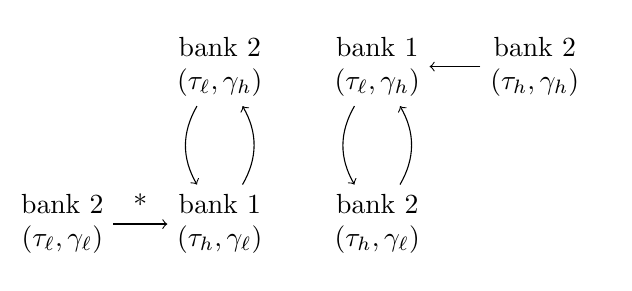
\begin{tikzpicture}
  % Nodes
    \hspace{-0.2cm}\node[align=center] (A) at (-2,0) {bank 2 \\ $(\tau_{\ell},\gamma_{\ell})$};
  \node[align=center] (B) at (0,0) {bank 1 \\ $(\tau_{h},\gamma_{\ell})$};
  \node[align=center] (C) at (2,0) {bank 2\\ $(\tau_{h},\gamma_{\ell})$};
  \node[align=center] (D) at (0,2) {bank 2\\ $(\tau_{\ell},\gamma_{h})$};
  \node[align=center] (E) at (2,2) {bank 1  \\ $(\tau_{\ell},\gamma_{h})$};
  \node[align=center] (F) at (4,2) {bank 2 \\ $(\tau_{h},\gamma_{h})$};
  % Arrows
  \draw[->] (A) -- node[above]{*} (B);
  %\draw[->,red] (D) -- (E);
  %\draw[->,red] (C) -- (B);
  %\draw[->,red] (F) -- (C);
  \draw[->,bend right] (B) to (D);
  \draw[->,bend right] (D) to (B);
  \draw[->,bend right] (E) to (C);
    \draw[->,bend right] (C) to (E);
    \draw[->] (F) to (E);
\end{tikzpicture} 
\caption{$\epsilon_1<0, \epsilon_2>0$.}
\end{minipage}
}
}
\resizebox{0.47\textwidth}{!}{    
\fbox{
\begin{minipage}{0.50\textwidth}
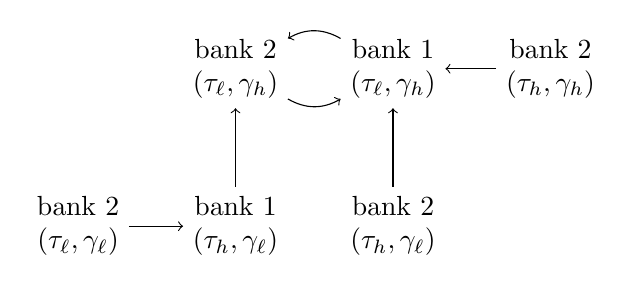
\begin{tikzpicture}
  % Nodes
    \node[align=center] (A) at (-2,0) {bank 2 \\ $(\tau_{\ell},\gamma_{\ell})$};
  \node[align=center] (B) at (0,0) {bank 1 \\ $(\tau_{h},\gamma_{\ell})$};
  \node[align=center] (C) at (2,0) {bank 2\\ $(\tau_{h},\gamma_{\ell})$};
  \node[align=center] (D) at (0,2) {bank 2\\ $(\tau_{\ell},\gamma_{h})$};
  \node[align=center] (E) at (2,2) {bank 1  \\ $(\tau_{\ell},\gamma_{h})$};
  \node[align=center] (F) at (4,2) {bank 2 \\ $(\tau_{h},\gamma_{h})$};
  % Arrows
  \draw[->] (A) -- (B);
  %\draw[->,red] (D) -- (E);
  %\draw[->,red] (C) -- (B);
  %\draw[->,red] (F) -- (C);
  \draw[->] (B) to (D);
  \draw[->] (C) to (E);
  \draw[->,bend right] (D) to (E);
    \draw[->,bend right] (E) to (D);
    \draw[->] (F) to (E);
\end{tikzpicture} 
\caption{$\epsilon_1>0, \epsilon_2>0$.}
\end{minipage}
}
}
\resizebox{0.47\textwidth}{!}{ 
\fbox{
\begin{minipage}{0.5\textwidth}
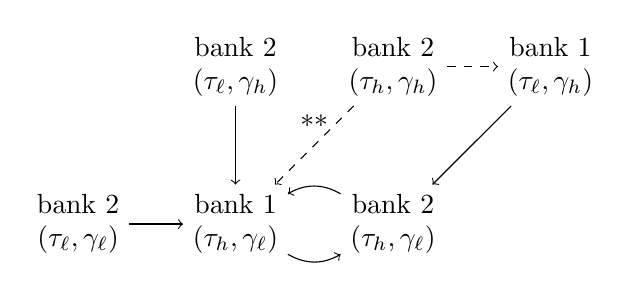
\begin{tikzpicture}
  % Nodes
    \node[align=center] (A) at (-2,0) {bank 2 \\ $(\tau_{\ell},\gamma_{\ell})$};
  \node[align=center] (B) at (0,0) {bank 1 \\ $(\tau_{h},\gamma_{\ell})$};
  \node[align=center] (C) at (2,0) {bank 2\\ $(\tau_{h},\gamma_{\ell})$};
  \node[align=center] (D) at (0,2) {bank 2\\ $(\tau_{\ell},\gamma_{h})$};
  \node[align=center] (E) at (2,2) {bank 2  \\ $(\tau_{h},\gamma_{h})$};
  \node[align=center] (F) at (4,2) {bank 1 \\ $(\tau_{\ell},\gamma_{h})$};
  % Arrows
  \draw[->] (A) -- (B);
  \draw[->] (F) -- (C);
  %\draw[->,red] (D) -- (E);
  %\draw[->,red] (C) -- (B);
  %\draw[->,red] (F) -- (C);
  \draw[->,dashed] (E) -- node[above]{**} (B);
  \draw[->,dashed] (E) -- (F);
  \draw[->] (D) to (B);
  \draw[->,bend right] (B) to (C);
    \draw[->,bend right] (C) to (B);
\end{tikzpicture} 
\caption{$\epsilon_1<0,\epsilon_2<0$.}
\end{minipage}
}
}
\resizebox{0.47\textwidth}{!}{ 
\fbox{
\begin{minipage}{0.5\textwidth}
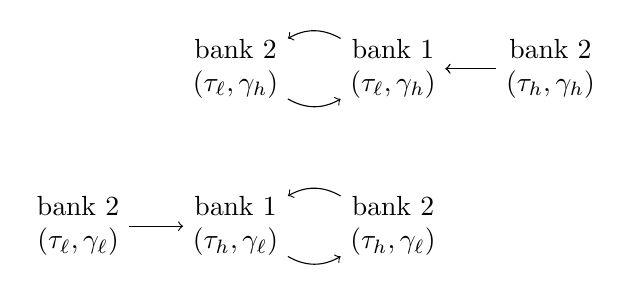
\begin{tikzpicture}
  % Nodes
    \node[align=center] (A) at (-2,0) {bank 2 \\ $(\tau_{\ell},\gamma_{\ell})$};
  \node[align=center] (B) at (0,0) {bank 1 \\ $(\tau_{h},\gamma_{\ell})$};
  \node[align=center] (C) at (2,0) {bank 2\\ $(\tau_{h},\gamma_{\ell})$};
  \node[align=center] (D) at (0,2) {bank 2\\ $(\tau_{\ell},\gamma_{h})$};
  \node[align=center] (E) at (2,2) {bank 1  \\ $(\tau_{\ell},\gamma_{h})$};
  \node[align=center] (F) at (4,2) {bank 2 \\ $(\tau_{h},\gamma_{h})$};
  % Arrows
  \draw[->] (A) -- (B);
  %\draw[->,red] (D) -- (E);
  %\draw[->,red] (C) -- (B);
  %\draw[->,red] (F) -- (C);
  \draw[->] (F) to (E);
  \draw[->,bend right] (B) to (C);
    \draw[->,bend right] (C) to (B);
     \draw[->,bend right] (D) to (E);
    \draw[->,bend right] (E) to (D);
    \draw[->] (F) to (E);
\end{tikzpicture} 
\caption{$\epsilon_1>0, \epsilon_2<0$.}
\end{minipage}
}
}
\caption{Alternative Best Response Dynamics. * The arrows means that, if bank 2 picks decision $(\tau_{\ell},\gamma_{\ell})$, the best response for Bank 1 is $(\tau_{h},\gamma_{\ell})$. ** The dashed arrow means that both case can happen, which depends on specific conditions on $D_y$. Note that it does not have an influence on the final conclusion, since both cases converge to the NE in the end. }
\label{fig:enter-label}
\end{figure}

% \subsection{Proof of Theorem \ref{thm:continous:peq}}
% \label{proof:continous}
% We first introduce the following simple lemma about the properties of $f$, which is easy to check.
% \begin{lemma}
% \label{lem:property of f}
% Assume $\emph{Supp}(D_y)=[0,1]$. We have
% \begin{enumerate}
%     \item $f(\gamma,\tau_a,\tau_b)$ is monotonically increasing with respect to $\gamma$. Moreover, let $y_{\gamma}=\frac{1}{2+\gamma}$, then $f(\gamma,y_{\gamma},\tau)$ is also monotonically increasing with respect to $\gamma$.
%     \item Let $\tau_a<\tau_b<\tau_c$. Then $f_{D_y}(\gamma_1,\tau_a,\tau_c)=f_{D_y}(\gamma_1,\tau_a,\tau_b)+f_{D_y}(\gamma_1,\tau_b,\tau_c)$.
%     \item Let $y_{\gamma}=\frac{1}{2+\gamma}$. If $y_{\gamma}\in(\tau_a,\tau_b)$, then $f(\gamma,\tau_a,y_{\gamma})<0$, and  $f(\gamma,y_{\gamma},\tau_b)>0$. 
% \end{enumerate}   
% \end{lemma}
% \noindent We analyze the existence of pure Nash equilibria under different conditions on the relationship between  decision pairs $\theta_1,\theta_2$. Firstly, note that, for a pair of $\theta_1,\theta_2$,  if the utility of a bank is strictly less than $0$, then the bank can always adjust its parameters $\gamma$ and $\tau$ to $1$ to ensure its utility becomes non-negative. This implies that decision pairs leading to non-positive utilities will not be an Nash equilibrium. Therefore, we only need to consider cases where $u_1 \geq 0$ and $u_2 \geq 0$.



% Next, we discuss the conditions for $\theta_1,\theta_2$ under which there are no pure NE under any distributions. We prove this by showing that, one can always find a new decision $\theta_1'=(\tau'_1,\gamma'_1)$ \textbf{or} $\theta_2'=(\tau'_2,\gamma'_2)$ for Bank 1 or 2 that leads to a larger utility for that bank.

% \paragraph{Case 1:} $\tau_1\leq \tau_2$, and $\gamma_1<\gamma_2$.
% In this case,   $u_1((\tau_1,\gamma_1),(\tau_2,\gamma_2))=f(\gamma_1,\tau_1,1),$ while $u_2=0.$ Let $\gamma_1'=\gamma_1+\epsilon<\gamma_2$ for some $\epsilon>0$. Then, $$u_1((\tau_1,\gamma_1'),(\tau_2,\gamma_2))=f(\gamma'_1,\tau_1,1)>f(\gamma_1,\tau_1,1)=u_1((\tau_1,\gamma_1),(\tau_2,\gamma_2)),$$ 
% where the inequality is based on the first property in Lemma \ref{lem:property of f}. It shows that $(\tau_1,\gamma_1')$ is a better decision for bank 1, therefor this case can not be a NE.   

% \paragraph{Case 2:} $\tau_1<\tau_2,\gamma_1=\gamma_2=\gamma$. In this case, $u_1((\tau_1,\gamma),(\tau_2,\gamma))=f(\gamma,\tau_1,\tau_2)+\frac{1}{2}f(\gamma,\tau_2,1)$, and $u_2((\tau_1,\gamma),(\tau_2,\gamma))=\frac{1}{2}f(\gamma,\tau_2,1)$. If $u_1((\tau_1,\gamma),(\tau_2,\gamma))=0,u_2((\tau_1,\gamma),(\tau_2,\gamma))>0$, then one can set $\tau_1'=\tau_2$, so that $$u_1((\tau_1',\gamma),(\tau_2,\gamma))=u_1((\tau_2,\gamma),(\tau_2,\gamma))=\frac{1}{2}f(\gamma,\tau_2,1)=u_2((\tau_1,\gamma),(\tau_2,\gamma))>0=u_1((\tau_1,\gamma),(\tau_2,\gamma)).$$
% If $u_1((\tau_1,\gamma),(\tau_2,\gamma))=u_2((\tau_1,\gamma),(\tau_2,\gamma))=0$, then it implies that $f(\gamma,\tau_1,\tau_2)=0$. Since $\text{Supp}(D_y)=[0,1]$, it means that there exists $\tau'\in(\tau_1,\tau_2)$ such that $f(\gamma,\tau_1,\tau')<0$ and $f(\gamma,\tau',\tau_2)>0$.  Therefore, if one sets $\tau_2'=\tau'$, we have 
% $$u_2((\tau_1,\gamma),(\tau'_2,\gamma))= f(\gamma,\tau',\tau_2)+\frac{1}{2}f(\gamma,\tau_2,1)>\frac{1}{2}f(\gamma,\tau_2,1)=u_2((\tau_1,\gamma),(\tau_2,\gamma)).$$
% \kri{Check these two subcases below, it's correct but I think some typo}
% If  $u_1((\tau_1,\gamma),(\tau_2,\gamma))>0$, $u_2((\tau_1,\gamma),(\tau_2,\gamma))=0$, it means that $f(\gamma,\tau_1,\tau_2)=0$. On the other hand, since $u_2=\frac{1}{2}f(\gamma,\tau_2,1)=\int_{\tau_2}^1[(2+\gamma)y-1]p(y)dy=0$, there exists a $\tau'\in(\tau_2,1)$, such that $(2+\gamma)\tau'-1=0$. Moreover, for all $\tau<\tau'$,  $(2+\gamma)\tau'-1<0$. This implies that $f(\gamma,\tau_1,\tau_2)<0$. This contradiction means that this case ($u_1((\tau_1,\gamma),(\tau_2,\gamma))>0$, $u_2((\tau_1,\gamma),(\tau_2,\gamma))=0$) will not happen. \\

% \noindent If $u_1((\tau_1,\gamma),(\tau_2,\gamma))>0$, and $u_2((\tau_1,\gamma),(\tau_2,\gamma))>0$, then let $y_{\gamma}=\frac{1}{2+\gamma}$. If $y_{\gamma}\in(\tau_1,\tau_2)$, then we have $f(\gamma,\tau_1,y_{\gamma})<0$, and $f(\gamma,y_{\gamma},\tau_2)>0$. Therefore, if one sets $\tau_1'=y_{\gamma}$, we have 
% $$u_1((\tau'_1,\gamma),(\tau_2,\gamma))=f(\gamma,y_{\gamma},\tau_2)>f(\gamma,\tau_1,y_{\gamma})+f(\gamma,y_{\gamma},\tau_2)=u_1((\tau_1,\gamma),(\tau_2,\gamma)).$$
% If $y_{\gamma}\geq \tau_2$, then we have $f(\gamma,\tau_1,\tau_2)< 0.$ Therefore, if we set $\tau_1'=\tau_2,$ we get 
% $$u_1((\tau_1',\gamma),(\tau_2,\gamma))=\frac{1}{2}f(\gamma,\tau_2,1)>f(\gamma,\tau_1,\tau_2)+\frac{1}{2}f(\gamma,\tau_2,1)>u_1((\tau_1,\gamma),(\tau_2,\gamma)).$$
% Similarly, if $y_{\gamma}\leq \tau_2$, setting $\tau_2'=\tau_1$ leads to a better utility for bank 2. 

% \paragraph{Case 3:} $\tau_1<\tau_2,$ $\gamma_1>\gamma_2$. In this case, $u_1((\tau_1,\gamma_1),(\tau_2,\gamma_2))=f(\gamma_1,\tau_1,\tau_2)$, and $u_2((\tau_1,\gamma),(\tau_2,\gamma))=f(\gamma_2,\tau_2,1)$. Let $y_{\gamma_{1}}=\frac{1}{2+\gamma_1}$, and $y_{\gamma_2}=\frac{1}{2+\gamma_2}$. Then, it is easy to check that if the pair of decisions will not be a NE if $\tau_1\not=y_{\gamma_{1}}$ or $\tau_2\not=y_{\gamma_{2}}$. \kri{We start by observing that for bank $2$ (with lower interest rate), it is optimal to set $\tau_2 = y_{\gamma_2}$ regardless of the other bank. Bank $2$ can always deviate to a threshold $y_{\gamma_2}$ and obtain higher utility, because if $y_{\gamma_2} < \tau_2$, it can drop threshold to $y_{\gamma_2}$ obtaining utility $f(\gamma_2, y_{\gamma_2}, 1) > f(\gamma_2, \tau_2, 1)$, similarly if $\tau_2 < y_{\gamma_2}$, bank 2 can increse threshold to $y_{\gamma_2}$ and get rid of the negative part of the integral}

% For example, if $\tau_1<y_{\gamma_{1}}$, then $f(\gamma_1,\tau_1,y_{\gamma_{1}})<0$, so setting $\tau_1'=y_{\gamma_{1}}$ leads to a larger utility for bank 1. For the case where $\tau_1=y_{\gamma_1}$ and $\tau_2=y_{\gamma_2}$, one can set $\gamma_2'=\gamma_2+\epsilon<\gamma_1$ for some $\epsilon>0$. In this case, 
% $$u_2((\tau_1,\gamma_1),(\tau_2,\gamma'_2))=f(\gamma_2',\tau_2,1)>f(\gamma_2,\tau_2,1)=u_2((\tau_1,\gamma_1),(\tau_2,\gamma_2)).$$


% Next, we discuss the case which can be a NE under certain conditions. 
% \paragraph{Case 4:} $\tau_1=\tau_2=\tau$, and $\gamma_1=\gamma_2=\gamma$. In this case, $u_1((\tau,\gamma),(\tau,\gamma))=u_2((\tau,\gamma),(\tau,\gamma))=\frac{1}{2}f(\gamma,\tau,1)$. Let $y_{\gamma}=\frac{1}{2+\gamma}$. If $y_{\gamma}>\tau$, then $f(\gamma,\tau,y)<0$, so if we sets $\tau'_2=y_{\gamma}$, we have 
% $$ u_2((\tau,\gamma),(\tau',\gamma))=\frac{1}{2}f(\gamma,y_{\gamma},1)>\frac{1}{2}f(\gamma,\tau,y_{\gamma})+\frac{1}{2}f(\gamma,y_{\gamma},1)=u_2((\tau,\gamma),(\tau,\gamma)).$$
% Similarly, if $y_{\gamma}<\tau$, we have $f(\gamma,y_{\gamma},\tau)>0$. Thus, we can set $\tau_2'=y_{\gamma}$, so 
% $$ u_2((\tau,\gamma),(\tau',\gamma))=\frac{1}{2}f(\gamma,y_{\gamma},1)>\frac{1}{2}f(\gamma,\tau,1)=u_2((\tau,\gamma),(\tau,\gamma)).$$
% The above discussion shows that this case will not be an NE if $\tau\not=y_{\gamma}.$ For the case where $\tau=y_{\gamma}$, we consider two possible situations: $\gamma>0$ and $\gamma=0$. If $\gamma>0$, then one can set $\gamma_1'=\gamma-\epsilon$ for a sufficiently small $\epsilon>0$, such that bank one double its profit with a very small cost (provided by $\epsilon$ is sufficiently small). If $\gamma=0$, then $\tau_1=\tau_2=y_{\gamma}=\frac{1}{2}$. In this case, no bank can double the profit by decreasing $\gamma$. Note that the game is symmetric, and the two players in this setting adopt the same decisions. Therefore, the decision pair $(\theta_1=(0.5,0),\theta_2=(0.5,0))$ will be an NE if and only if  
% $$u_1(\theta_1,\theta_2)\geq u_1(\theta'_1=(\tau',\gamma'),\theta_2),$$
% for any other $\theta_1'\in[0,1]^2$. If $\tau'>\tau$ and $\gamma'=\gamma$, then 
% $$u_1((\tau',\gamma'),\theta_2)=\frac{1}{2}f(\gamma,\tau',1)=\frac{1}{2}[f(\gamma,\tau,1) -f(\gamma,\tau,\tau')]<u_1(\theta_1,\theta_2),$$
% since $f(\gamma,\tau,\tau')>0$ by the definition of $y_{\gamma}.$
% If $\tau'<\tau$ and $\gamma'=\gamma$, then 
% $$u_1((\tau',\gamma'),(\tau,\gamma))=\frac{1}{2}f(\gamma,\tau',1)=\frac{1}{2}[f(\gamma,\tau'\tau)+f(\gamma,\tau,1)]<u_1(\theta_1,\theta_2),$$
% as $f(\gamma,\tau',\tau)<0.$ If $\tau'\geq\tau$ and $\gamma'>\gamma$, then $u_1((\tau',\gamma'),\theta_2)=0<u_1((\tau,\gamma),\theta_2)$. Finally, we consider the case where $\tau'<\tau$, and $\gamma'>\gamma$. In this case, 
% $$u_1((\tau',\gamma'),\theta_2)=\int^{\tau}_{\tau'}[(2+\gamma')y-1]p(y)dy.$$
% We have for all $(\tau',\gamma')$ such that $\tau'<\tau$ and $\gamma'>\gamma$, 
% $$\int^{\tau}_{\tau'}[(2+\gamma')y-1]p(y)dy\leq \int^{\tau}_{\tau'}[(2+1)y-1]p(y)dy\leq  \int^{\tau}_{y_1=\frac{1}{2+1}}[(2+1)y-1]p(y)dy=f\left(1,\frac{1}{3},0.5\right).$$
% This implies that, for all $(\tau',\gamma')$ such that $\tau'<\tau$ and $\gamma'>\gamma$, the maximum utility of bank 1 is achieved when $\tau'=\frac{1}{3}$, and $\gamma'=0.5$ \kri{$\gamma' = 1$ right?}. Therefore, $u_1(\theta_1,\theta_2)\geq u_1(\theta'_1=(\tau',\gamma'),\theta_2)$ if and only if 
% $$\frac{1}{2} f(0,0.5,1)\geq f\left(1,\frac{1}{3},0.5\right),$$
% \kri{Edited above}
% which finishes the proof. 



\subsection{Proof of Theorem \ref{thm:mixed-NE}}
\label{Proof:Theorem:mixedNE}
We overload notation and denote the expected utility of bank $i$ under $p_1$ and $p_2$ as:
$$ u_{i}(p_1,p_2)=\E_{\theta_1\sim p_1, \theta_2\sim p_2}[u_i(\theta_1,\theta_2)]. $$


\noindent Firstly, note that, based on Table \ref{tab:my-table} and Lemma \ref{lem:property of f}, it can be easily shown that for any $\theta\in\{\theta^{(j)}\}_{j=1}^4$, 
$$u_1(\theta^{(3)},\theta)> u_1(\theta^{(1)},\theta). $$
More specifically, 
\begin{equation*}
    \begin{split}
u_1(\theta^{(3)},\theta^{(1)})={} & \frac{1}{2}f(\gamma_{\ell},\tau_{h},1)>\frac{1}{2}f(\gamma_{\ell},\tau_{\ell},1) =   u_1(\theta^{(1)},\theta^{(1)}),\\
u_1(\theta^{(3)},\theta^{(2)})={} & f(\gamma_{\ell},\tau_{h},1)>f(\gamma_{\ell},\tau_{\ell},1) =   u_1(\theta^{(1)},\theta^{(2)}),\\
u_1(\theta^{(3)},\theta^{(3)})={} & \frac{1}{2}f(\gamma_{\ell},\tau_{h},1)>f(\gamma_{\ell},\tau_{\ell},\tau_h)+\frac{1}{2}f(\gamma_{\ell},\tau_h,1) =   u_1(\theta^{(1)},\theta^{(3)}),\\
u_1(\theta^{(3)},\theta^{(4)})={} & f(\gamma_{\ell},\tau_{h},1)>f(\gamma_{\ell},\tau_{\ell},1) =   u_1(\theta^{(1)},\theta^{(4)}),
    \end{split}
\end{equation*}
where the first, second and last inequality is because based on Lemma \ref{lem:property of f}, 
$$f(\gamma_{\ell},\tau_{\ell},1)=\underbrace{f(\gamma_{\ell},\tau_{\ell},\tau_{h})}_{<0}+f(\gamma_{\ell},\tau_{h},\tau_{h}),$$
and the third inequality is because $f(\gamma_{\ell},\tau_{\ell},\tau_{h})<0.$ This implies that $\theta^{(1)}$ is strictly dominated by $\theta^{(3)}$, and will not be part of the mixed NE. 


Since the game is symmetric, the same argument holds true for Bank 2, i.e. $u_2(\theta,\theta^{(3)}) > u_2(\theta,\theta^{(1)})$. By a similar argument, for any $\theta\in\{\theta^{(j)}\}_{j=2}^4$, we have
$$u_1(\theta^{(2)},\theta)> u_1(\theta^{(4)},\theta), $$
which indicates that $\theta^{(4)}$ will also not be part of mixed NE for Bank 1 or Bank 2.  To summarize, any mixed NE must satisfy $p_{1,1}=p_{1,4}=p_{2,1}=p_{2,4}=0$.\\


\noindent Consider a pair of mixed strategies $p_1=[0,p_{1,2},1-p_{1,2},0]$ and $p_2=[0,p_{2,2},1-p_{2,2},0]$. Then the utility of Bank 1 can be written as: 
\begin{equation}
    \begin{split}
    \label{eqn:u13123123}
u_{1}(p_1,p_2) = {} & \frac{1}{2} p_{1,2}p_{2,2} f(\gamma_{h}, \tau_{\ell}, 1) + p_{1,2}(1-p_{2,2})f(\gamma_{h},\tau_{\ell},\tau_{h})+ (1-p_{1,2})p_{2,2}f(\gamma_{\ell},\tau_h,1)\\
{} & + \frac{(1-p_{1,2})(1-p_{2,2})}{2}f(\gamma_{\ell},\tau_{h},1)\\       = {} & \frac{1}{2}p_{1,2}\left[(2-p_{2,2})f(\gamma_{h},\tau_{\ell},\tau_{h}) + p_{2,2}f(\gamma_{h},\tau_{h},1) -(1+p_{2,2})f(\gamma_{\ell},\tau_{h},1) \right] \\
{} & + \frac{(p_{2,2}+1)}{2}f(\gamma_{\ell},\tau_{h},1).
    \end{split}
\end{equation}
Note that it is a linear function with respect to $p_{1,2}$, and the slope is given by:
\begin{equation*}
    \begin{split}
        {} & \frac{1}{2} \left[(2-p_{2,2})f(\gamma_{h},\tau_{\ell},\tau_{h}) + p_{2,2}f(\gamma_{h},\tau_{h},1) -(1+p_{2,2})f(\gamma_{\ell},\tau_{h},1)\right]\\
        = {} & \frac{1}{2} p_{2,2}[f(\gamma_{h},\tau_{h},1)-f(\gamma_{\ell},\tau_{h},1)-f(\gamma_{h},\tau_{\ell},\tau_{h})] + f(\gamma_{h},\tau_{\ell},\tau_{h}) - \frac{1}{2} f(\gamma_{\ell},\tau_{h},1),
    \end{split}
\end{equation*}
Let 
\begin{equation}
\label{eqn:def-of-g(p)}
g(p)=p[f(\gamma_{h},\tau_{h},1)-f(\gamma_{\ell},\tau_{h},1)-f(\gamma_{h},\tau_{\ell},\tau_{h})] + 2f(\gamma_{h},\tau_{\ell},\tau_{h}) - f(\gamma_{\ell},\tau_{h},1).
\end{equation}
Then, the slope of $u(p_1,p_2)$ with respect to $p_{1,2}$ is given by $\frac{1}{2} g(p_{2,2})$.
Moreover, (recalling our definitions of the shorthand notation $\epsilon_1 = \frac{1}{2} f(\gamma_h, \tau_{\ell},1) - f(\gamma_{\ell},\tau_h, 1)$ and $\epsilon_2 = f(\gamma_h, \tau_{\ell}, \tau_h) - \frac{1}{2} f(\gamma_{\ell},\tau_h, 1)$), we note that $g(p):[0,1]\mapsto \R$ is a linear function, $g(0)=2\epsilon_2$, and $g(1)=2\epsilon_1$.
\\
\noindent 

Let $BR_1(p) \subseteq [0,1]$ denote the candidate set of best response probabilities of picking $\theta^{(2)}$ of Bank 1 if Bank 2 picks $p_2=[0,p,1-p,0]$. 
The corresponding candidate set for Bank 2 is denoted by $BR_2(p)$.

Then, consider the following cases: 

\noindent \paragraph{Case 1:} $\epsilon_1<0$, $\epsilon_2<0$. Therefore, $g(0)=2\epsilon_2<0$ and  $g(1)=2\epsilon_1<0$, 
then it is clear that $g(p)<0$ for all $p\in[0,1]$. 
This means that the slope in \eqref{eqn:u13123123} will always be negative, so $BR_1(p)= \{0\}$ for any $p\in[0,1]$. Similarly, $BR_2(p)=\{0\}$ for any $p\in[0,1]$, which indicates that $p_{1,2}=p_{2,2}=0$, $p_{1,3}=p_{2,3}=1$ is the only mixed NE (and, in fact, this corresponds to a pure NE).

\noindent \paragraph{Case 2:} $\epsilon_1<0$, $\epsilon_2>0$. Therefore, $g(0)>0$, and $g(1)<0$, and since $g$ is a linear function, it means that there must exist a unique $c\in(0,1)$, such that $g(c)=0$. Based on \eqref{eqn:def-of-g(p)}, we know 
$$ c=\frac{f(\gamma_{\ell},\tau_h,1)-2f(\gamma_h,\tau_{\ell},\tau_h)}{f(\gamma_h,\tau_h,1)-f(\gamma_{\ell},\tau_h,1)-f(\gamma_h,\tau_{\ell},\tau_h)}.$$
Combining with \eqref{eqn:u13123123}, we have 
\begin{equation*}
BR_1(p)= 
    \begin{cases}
        \{0\}, & p>c;\\
        \{1\},  & p<c;\\
        [0,1], & p=c.
    \end{cases}
\end{equation*}
This is because, if $p>c$, $g(p)<0$, so the slope in \eqref{eqn:u13123123} is negative, and $BR_1(p)=\{0\}$.If $p<c$, then $g(p)>0$, the slope in \eqref{eqn:u13123123} is positive, and $BR_1(p)=\{1\}$. If $p=c$, \eqref{eqn:u13123123} will not be a function of $p_{1,2}$, so any decision for Bank 1 leads to the same gain. Similarly, we have 
\begin{equation*}
BR_2(p)= 
    \begin{cases}
        \{0\}, & p>c;\\
        \{1\},  & p<c;\\
        [0,1], & p=c.
    \end{cases}
\end{equation*}
Therefore, we know that $([0,c,1-c,0],[0,c,1-c,0])$ is a mixed NE, and $([0,0,1,0],[0,1,0,0])$ and $([0,1,0,0],[0,0,1,0])$ are also pure NEs. 

\noindent \paragraph{Case 3:} $\epsilon_1>0$, $\epsilon_2<0$. Therefore, $g(0)<0$, and $g(1)>0$, and since $g$ is a linear function, it means that there must exist $c\in(0,1)$, such that $g(c)=0$. 
Combining with \eqref{eqn:u13123123}, we have 
\begin{equation*}
BR_1(p)= 
    \begin{cases}
        \{1\}, & p>c;\\
        \{0\},  & p<c;\\
        [0,1], & p=c.
    \end{cases}
\end{equation*}
Similarly, we have 
\begin{equation*}
BR_2(p)= 
    \begin{cases}
        \{1\}, & p>c;\\
        \{0\},  & p<c;\\
        [0,1], & p=c.
    \end{cases}
\end{equation*}
Therefore, we know that $([0,c,1-c,0],[0,c,1-c,0])$ is a mixed NE, and $([0,0,1,0],[0,0,1,0])$ and $([0,1,0,0],[0,1,0,0])$ are also pure NEs. 

\noindent \paragraph{Case 4:} $\epsilon_1>0$, $\epsilon_2>0$. In this case, we know that $g(p)>0$ for all $p\in[0,1]$. Then, we have $BR_1(p)=\{1\}$, and $BR_2(p)=\{1\}$, which implies that the only mixed NE here is $([0,1,0,0], [0,1,0,0])$ (which is in fact a pure NE).
This completes the proof of the theorem.

\subsection{Proof of Theorem \ref{thm:cE}}
\label{proof:CE}

Firstly, we know $u_i(\theta^{(3)},\theta)> u_i(\theta^{(1)},\theta),$. This means $\theta^{(1)}$ will not be part of CE. Conditioned on this, for any $\theta\in\{\theta^{(j)}\}_{j=2}^4$, we have
$u_1(\theta^{(2)},\theta)> u_1(\theta^{(4)},\theta).$ This indicates that $\theta^{(4)}$ will no be part of CE. Thus, $p_{11}=\dots,=p_{14}=0$, $p_{11}=\dots,=p_{41}=0$, $p_{14}=\dots,=p_{44}=0$, $p_{41}=\dots,=p_{44}=0$. Next, based on Definition \ref{defn:CE}, we firstly need:
\begin{equation*}
    \begin{split}
     \sum_{i=2}^3 u_1\left((\tau_{\ell},\gamma_{h}),\theta^{(i)}\right)p_{2i} \geq {} &    \sum_{i=2}^3 u_1\left(\theta',\theta^{(i)}\right)p_{2i},\ \forall \theta'\in\Theta, 
    \end{split}
\end{equation*}
That is, for $\theta'=\theta^{(1)}$,
\begin{equation*}
    \begin{split}
 p_{22}\frac{1}{2}f(\gamma_h,\tau_{\ell},1) + p_{23} f(\gamma_h,\tau_{\ell},\tau_{h}) \geq  p_{22} f(\gamma_{\ell},\tau_{\ell},1) + p_{23} (f(\gamma_{\ell},\tau_{\ell},\tau_h)+\frac{1}{2}f(\gamma_{\ell},\tau_h,1)),     
    \end{split}
\end{equation*}
that is, 
$$ p_{22}(\epsilon_1-f(\gamma_{\ell},\tau_{\ell},\tau_h) )\geq p_{23}(f(\gamma_{\ell},\tau_{\ell},\tau_h)-\epsilon_2  ),$$
that is 
\begin{equation}
\label{eqn:ce:drop1}
    p_{22}\epsilon_1 \geq -p_{23}\epsilon_2 + (p_{22}+p_{23})f(\gamma_{\ell},\tau_{\ell},\tau_h). 
\end{equation}
For $\theta'=\theta^{(3)}$, we have 
\begin{equation}
\label{eqn:ce:nodrop1}
     p_{22}\epsilon_1 \geq  -p_{23}\epsilon_2.
\end{equation}
Note that since 
$f(\gamma_{\ell},\tau_{\ell},\tau_h)$ is negative, we know that \eqref{eqn:ce:nodrop1} implies \eqref{eqn:ce:drop1}, and thus \eqref{eqn:ce:drop1} can be dropped. 

For $\theta'=\theta^{(4)}$, we have 
\begin{equation*}
    \begin{split}
 p_{22}\frac{1}{2}f(\gamma_h,\tau_{\ell},1) + p_{23} f(\gamma_h,\tau_{\ell},\tau_{h}) \geq  p_{22} \frac{1}{2}f(\gamma_{h},\tau_h,1) + p_{23} 0,     
    \end{split}
\end{equation*}
which always holds true. Next, we need 
\begin{equation*}
    \begin{split}
     \sum_{i=2}^3 u_1\left((\tau_{h},\gamma_{\ell}),\theta^{(i)}\right)p_{3i} \geq {} &    \sum_{i=2}^3 u_1\left(\theta',\theta^{(i)}\right)p_{3i},\ \forall \theta'\in\Theta. 
    \end{split}
\end{equation*}
For $\theta'=\theta^{(1)}$, it means 
$$p_{32} f(\gamma_{\ell},\tau_{h},1) + p_{33}\frac{1}{2}f(\gamma_{\ell},\tau_h,1)\geq p_{32} f(\gamma_{\ell},\tau_{\ell},1) + p_{33} \left(f(\gamma_{\ell},\tau_{\ell},\tau_h)+\frac{1}{2}f(\gamma_{\ell},\tau_h,1)\right), $$
which always holds true. For $\theta'=\theta^{(2)}$, we have 
$$ -p_{32}\epsilon_1\geq p_{33}\epsilon_2.$$
For $\theta'=\theta^{(4)}$, we have 
$$ p_{32} f(\gamma_{\ell},\tau_{h},1) + p_{33}\frac{1}{2}f(\gamma_{\ell},\tau_h,1) \geq p_{32} \frac{1}{2} f(\gamma_{h},\tau_h,1). $$
Rearrange, we have
$$ -p_{32}\epsilon_1\geq p_{33}\epsilon_2 -\left(p_{33}+\frac{1}{2}p_{32}\right)f(\gamma_{h},\tau_{\ell},\tau_h). $$
Since $f(\gamma_{h},\tau_{\ell},\tau_h)$ is positive, the above condition is implied by $ -p_{32}\epsilon_1\geq p_{33}\epsilon_2,$ and thus can be dropped. 

To proceed, we need 
\begin{equation*}
    \begin{split}
     \sum_{i=2}^3 u_2\left(\theta^{(i)},(\tau_{\ell},\gamma_{h})\right)p_{i2} \geq {} &    \sum_{i=2}^3 u_2\left(\theta^{(i)},\theta'\right)p_{i2},\ \forall \theta'\in\Theta, 
    \end{split}
\end{equation*}
which is equivalent to 
\begin{equation*}
    \begin{split}
     \sum_{i=2}^3 u_1\left((\tau_{\ell},\gamma_{h}),\theta^{(i)}\right)p_{i2} \geq {} &    \sum_{i=2}^3 u_1\left(\theta',\theta^{(i)}\right)p_{i2},\ \forall \theta'\in\Theta. 
    \end{split}
\end{equation*}
Thus, following similar procedure, the condition we get is 
$$ p_{22}\epsilon_1\geq -p_{32}\epsilon_2. $$
Finally, for 
\begin{equation*}
    \begin{split}
     \sum_{i=2}^3 u_2\left(\theta^{(i)},(\tau_{h},\gamma_{\ell})\right)p_{i3} \geq {} &    \sum_{i=2}^3 u_2\left(\theta^{(i)},\theta'\right)p_{i3},\ \forall \theta'\in\Theta, 
    \end{split}
\end{equation*}
we get 
$$ -p_{23}\epsilon_1\geq p_{33}\epsilon_2,$$
To summarize, we have the following conditions:
\begin{align}
        p_{22}\epsilon_1 \geq {} & -p_{23}\epsilon_2 \label{eq:first}\\
        -p_{32}\epsilon_1\geq {} & p_{33}\epsilon_2 \label{eq:second}.\\
        p_{22}\epsilon_1\geq {} & -p_{32}\epsilon_2 \label{eq:fourth}\\
         -p_{23}\epsilon_1\geq {} & p_{33}\epsilon_2 \label{eq:fifth},
\end{align}
When $\epsilon_1>0$ and $\epsilon_2>0$, from \eqref{eq:second} and \eqref{eq:fifth}, we know that $p_{32}=p_{33}=p_{23}=0$, which leads to $p_{22}=1$, and it can make sure all inequality is ture. Similarly,  when $\epsilon_1<0$ and $\epsilon_2<0$, we get $p_{22}=p_{32}=p_{23}=0$, and $p_{33}=1$.

When $\epsilon_1>0,\epsilon_2<0$,  we need $\min\{p_{22},p_{33}\}>\max\left\{ \frac{|\epsilon_2|}{\epsilon_1}p_{23}, \frac{\epsilon_1}{|\epsilon_2|}p_{32} \right\}$. For  $\epsilon_1<0$ and $\epsilon_2>0$, we need $\min\{p_{23},p_{32}\}>\max\left\{ \frac{|\epsilon_1|}{\epsilon_2}p_{22}, \frac{\epsilon_2}{|\epsilon_1|}p_{33} \right\}$. 




\section{Proofs for Section~\ref{sec:learntoconvege}: Convergence of Dynamics}



\subsection{Proof of Lemma \ref{lem:1 and 4 p}}
\label{proof:Lemma: converofp_1p_4}
We have for $t>1$,
\begin{equation*}
\begin{split}
    \frac{p^{(t+1)}_{1,1}}{p^{(t+1)}_{1,3}}  = {} & \frac{p^{(t)}_{1,1}\exp\left(\eta \sum_{j=1}^4 p_{2,j}^{(t)}u_1\left(\theta^{(1)},\theta^{(j)}\right) \right)}{p^{(t)}_{1,3}\exp\left(\eta \sum_{j=1}^4 p_{2,j}^{(t)}u_1\left(\theta^{(3)},\theta^{(j)}\right) \right)} = \frac{p_{1,1}^{(t)}}{p_{1,3}^{(t)}}\exp\left(\eta \sum_{j=1}^4p_{2,j}^{(t)}\left(u_1\left(\theta^{(1)},\theta^{(j)}\right)-u_1\left(\theta^{(3)},\theta^{(j)}\right)\right)\right) \\
\leq {} &  \frac{p_{1,1}^{(t)}}{p_{1,3}^{(t)}}\exp\left(-\eta\xi_1\right),
\end{split}
\end{equation*}
where recall that we defined $\xi_1 := \min\{\frac{1}{2}\left|f(\gamma_{\ell},\tau_{\ell},\tau_{h})\right|,\frac{1}{2}|f(\gamma_{h},\tau_{\ell},\tau_{h})|, |\epsilon_1|, |\epsilon_2|\}>0$ as shorthand.
Therefore, we have 
\[
{p^{(t+1)}_{1,1}}\leq p_{1,3}^{(t+1)} \frac{p^{(1)}_{1,1}}{p^{(1)}_{1,3}}\left[\exp\left(-\eta\xi_1\right)\right]^{t}\leq  \frac{p^{(1)}_{1,1}}{p^{(1)}_{1,3}}\left[\exp\left(-\eta\xi_1\right)\right]^{t}\leq c_{ini}\left[\exp\left(-\eta\xi_1\right)\right]^{t},
\]
where the last inequality plugs in the definition of $c_{ini}=\max_{i\in[2]}\left\{\frac{\max_{j\in[4]}p^{(1)}_{i,j}}{\min_{i\in[4]}p^{(1)}_{i,j}}\right\}$.
Similarly, we also have 

\begin{equation*}
\begin{split}
    \frac{p^{(t+1)}_{2,1}}{p^{(t+1)}_{2,3}}  = {} & \frac{p^{(t)}_{2,1}\exp\left(\eta \sum_{j=1}^4 p_{1,j}^{(t)}u_2\left(\theta^{(j)},\theta^{(1)}\right) \right)}{p^{(t)}_{2,3}\exp\left(\eta \sum_{j=1}^4 p_{1,j}^{(t)}u_2\left(\theta^{(j)},\theta^{(3)}\right) \right)} = \frac{p_{2,1}^{(t)}}{p_{2,3}^{(t)}}\exp\left(\eta \sum_{j=1}^4p_{1,j}^{(t)}\left(u_1\left(\theta^{(1)},\theta^{(j)}\right)-u_1\left(\theta^{(3)},\theta^{(j)}\right)\right)\right) \\
\leq {} &  \frac{p_{2,1}^{(t)}}{p_{2,3}^{(t)}}\exp\left(-\eta\xi_1\right),
\end{split}
\end{equation*}
where the second equality is based on the fact the game is symmetric. It implies that 
\[
{p^{(t+1)}_{2,1}}\leq c_{ini}\left[\exp\left(-\eta\xi_1\right)\right]^{t}.
\]
Next, we know that $u_1(\theta^{(2)},\theta^{(1)})=u_1(\theta^{(4)},\theta^{(1)})=0$, but for all $j \neq 1$, we have $u_1\left(\theta^{(2)},\theta^{(j)}\right) - u_1\left(\theta^{(4)},\theta^{(j)}\right) \geq \xi_1$. Therefore, we have for all $t>1$,
\begin{equation}\label{eq:recursive-p14}
   \begin{split}
\frac{p^{(t+1)}_{1,4}}{p^{(t+1)}_{1,2}} =      \frac{p^{(t)}_{1,4}}{p^{(t)}_{1,2}} \exp\left(\eta \sum_{j=2}^4 p^{(t)}_{2,j}\left(u_1\left(\theta^{(4)},\theta^{(j)}\right)-u_1\left(\theta^{(2)},\theta^{(j)}\right)\right) \right)\leq \frac{p^{(t)}_{1,4}}{p^{(t)}_{1,2}} \exp\left(-\eta \xi_1\sum_{j=2}^4 p^{(t)}_{2,j} \right).
   \end{split} 
\end{equation}
Note that it implies that the ratio between $p_{1,4}^{(t)}$ and $p_{1,2}^{(t)}$ is non-increasing. Moreover, we have just shown that
\[
p_{2,1}^{(t)}\leq c_{ini}\exp\left(-\eta\xi_1(t-1)\right)
\]
For $t\geq t'=\max\left\{\left\lceil\frac{\log 2c_{ini}}{\epsilon\eta}+1\right\rceil,2\right\}$, we have $p_{2,1}^{(t)}\leq \frac{1}{2}$, which implies that 
\[
\sum_{j=2}^4p_{2,j}^{(t)}= 1- p_{1,2}^{(t)}\geq\frac{1}{2}.
\] 
Thus, 
\begin{equation*}
    \begin{split}
 \frac{p^{(t+1)}_{1,4}}{p^{(t+1)}_{1,2}}\leq {} &  \frac{p^{(t)}_{1,4}}{p^{(t)}_{1,2}} \exp\left(-\eta \xi_1\sum_{j=2}^4 p^{(t)}_{2,j} \right)\leq \frac{p^{(t'-1)}_{1,4}}{p^{(t'-1)}_{1,2}} \left(\exp\left(-\frac{1}{2}\eta \xi_1 \right)\right)^{t-t'+1}\exp\left(-\eta\xi_1\sum_{j=2}^4p_{2,j}^{(t'-1)}\right)\\
\leq {} &\frac{p^{(1)}_{1,4}}{p^{(1)}_{1,2}} \left(\exp\left(-\frac{1}{2}\eta \xi_1 \right)\right)^{t-t'+1}\leq c_{ini}\exp\left(-\frac{1}{2}\eta \xi_1(t-t'+1) \right).       
    \end{split}
\end{equation*}
where the penultimate inequality uses Equation~\eqref{eq:recursive-p14} recursively for $t = t' - 1, \ldots, 1$. We complete the proof by setting 
$$c_{ini}\exp\left(-\frac{1}{2}\eta \xi_1(t-t'+1) \right)\leq\omega. $$

%This completes the proof of the lemma.

\subsection{Proof of Theorem 4}
\label{proof:Theoerm:conveccc}
In this section, we present the proof of Theorem 4, considering four cases based on the different possible signs of $\epsilon_1$ and $\epsilon_2$.\\
Recall the definitions $\epsilon_1 = \frac{1}{2} f(\gamma_h, \tau_{\ell},1) - f(\gamma_{\ell},\tau_h, 1)$ and $\epsilon_2 = f(\gamma_h, \tau_{\ell}, \tau_h) - \frac{1}{2} f(\gamma_{\ell},\tau_h, 1)$.
Also recall the shorthand definitions $\xi_1=\min\{\frac{1}{2}f(\gamma_{\ell},\tau_{h},1), \frac{1}{2}\left|f(\gamma_{\ell},\tau_{\ell},\tau_{h})\right|,\frac{1}{2}|f(\gamma_{h},\tau_{\ell},\tau_{h})|, |\epsilon_1|, |\epsilon_2|\}>0$ and $c_{ini} := \max_{i\in[2]}\left\{\frac{\max_{j\in[4]}p^{(1)}_{i,j}}{\min_{i\in[4]}p^{(1)}_{i,j}}\right\}$.


\noindent \textbf{Case I: $\epsilon_1<0,$ and $\epsilon_2<0$.} We have 
\begin{equation}
    \begin{split}
    \label{eqn:throrem 4:case1}
     \frac{p^{(t+1)}_{1,2}}{p^{(t+1)}_{1,3}}  = {} &  \frac{p^{(t)}_{1,2}}{p^{(t)}_{1,3}}\exp\left(\eta \sum_{j=1}^4 p^{(t)}_{2,j}\left(u_1\left(\theta^{(2)}, \theta^{(j)}\right)-u_1\left(\theta^{(3)}, \theta^{(j)}\right)\right)\right) \\ 
     \leq  {} &  \frac{p^{(t)}_{1,2}}{p^{(t)}_{1,3}}\exp\left( -\eta \sum_{j=1}^3p^{(t)}_{2,j}\xi_1 + p^{(t)}_{2,4}\left(f(\gamma_{h},\tau_{\ell},\tau_{h})+\frac{1}{2}f(\gamma_{h},\tau_{h},1)-f(\gamma_{\ell},\tau_h,1)\right)  \right)\\
     \leq {} &  \frac{p^{(t)}_{1,2}}{p^{(t)}_{1,3}}\exp\left( -\eta \sum_{j=1}^3p^{(t)}_{2,j}\xi_1 + 3\eta p^{(t)}_{2,4}  \right)
     =  \frac{p^{(t)}_{1,2}}{p^{(t)}_{1,3}}\exp\left( -\eta \sum_{j=1}^4p^{(t)}_{2,j}\xi_1 + \eta(\xi_1+3) p^{(t)}_{2,4}  \right)\\
     = {} &  \frac{p^{(t)}_{1,2}}{p^{(t)}_{1,3}}\exp\left( -\eta\xi_1 + \eta(\xi_1+3) p^{(t)}_{2,4}  \right).\\
    \end{split}
\end{equation}
For the first inequality, it is because:
\begin{equation*}
    \begin{split}
u_1(\theta^{(2)},\theta^{(1)})-u_1(\theta^{(3)},\theta^{(1)})={} & 0-\frac{1}{2}f(\gamma_{\ell},\tau_{h},1)\leq -\xi_1,\\
u_1(\theta^{(2)},\theta^{(2)})-u_1(\theta^{(3)},\theta^{(2)})={} & \frac{1}{2}f(\gamma_{h},\tau_{\ell},1)-f(\gamma_{\ell},\tau_{h},1)=\epsilon_1\leq -\xi_1,\\
u_1(\theta^{(2)},\theta^{(3)})-u_1(\theta^{(3)},\theta^{(3)})={} &f(\gamma_{h},\tau_{\ell},\tau_{h})- \frac{1}{2}f(\gamma_{\ell},\tau_{h},1)=\epsilon_2\leq -\xi_1.
    \end{split}
\end{equation*}
The second inequality of \eqref{eqn:throrem 4:case1} is because the $f$ function is upper bounded by 2 based on Lemma \ref{lem:property of f}, and $f(\gamma_{\ell},\tau_{h},1)$ is positive. Denote as shorthand the constant $t''=t'+1+\left\lceil\frac{2}{\eta\xi_1}\log\frac{2(\xi_1+3)c_{ini}}{\xi_1}\right\rceil$.
Then, from Lemma \ref{lem:1 and 4 p}, we have for $t\geq t''$, 
$$\eta(\xi_1+3)p_{2,4}^{(t)}\leq \frac{\eta\xi_1}{2}.$$
Thus, we have  
\begin{equation*}
    \begin{split}
   \frac{p^{(t+1)}_{1,2}}{p^{(t+1)}_{1,3}} 
   \leq {} & \frac{p^{(t)}_{1,2}}{p^{(t)}_{1,3}} \exp\left(-\frac{\eta\xi_1}{2}\right) \ldots \leq \frac{p^{(t''-1)}_{1,2}}{p^{(t''-1)}_{1,3}} \left[\exp\left(-\frac{\eta\xi_1}{2}\right)\right]^{t-t''+1}\\
   \leq {} & c_{\text{ini}}\exp\left(3\eta t''\right)\exp\left(-\frac{\eta\xi_1}{2}\left(t-t''+1\right)\right),     
    \end{split}
\end{equation*}
where the last inequality is obtained by applying the following inequality recursively for $t=t''-1,\dots,1$:
$$  \frac{p^{(t)}_{1,2}}{p^{(t)}_{1,3}}  \leq  \frac{p^{(t-1)}_{1,2}}{p^{(t-1)}_{1,3}}\exp\left( -\eta\xi_1 + \eta(\xi_1+3) p^{(t-1)}_{2,4}  \right)\leq \frac{p^{(t-1)}_{1,2}}{p^{(t-1)}_{1,3}} \exp(3\eta),$$
which is obtained based on \eqref{eqn:throrem 4:case1}.

Note that $t''$ is a constant. We have for $t\geq t''$,
$$p^{(t+1)}_{1,2}\leq c_{\text{ini}}\exp\left(3\eta t''\right)\exp\left(-\frac{\eta\xi_1}{2}\left(t-t''+1\right)\right), $$ 
and thus 
$$ p^{(t+1)}_{1,3}\geq \max\left\{ 1 -3c_{\text{ini}}\exp\left(3\eta t''\right)\exp\left(-\frac{\eta\xi_1}{2}\left(t-t''+1\right)\right),0\right\} $$
The proof is completed by setting 
$$c_{\text{ini}}\exp\left(3\eta t''\right)\exp\left(-\frac{\eta\xi_1}{2}\left(t-t''+1\right)\right)\leq \omega.$$
It shows that $p_{1,2}^{(t)}$ converges to 0 at an exponential rate after $t''$ iterations, which is a constant factor. Combining with Lemma \ref{lem:1 and 4 p}, we can draw the conclusion that $p_{1,3}^{(t)}$ converges to 1 exponentially fast after a constant number of iterations.
An identical argument reaches the same conclusion for Bank 2.
This implies that the algorithm eventually converges to the symmetric pure NE $((\tau_h, \gamma_{\ell}),(\tau_h, \gamma_{\ell}))$.
\\


\noindent \textbf{Case II: $\epsilon_1>0,$ and $\epsilon_2>0$.} 
The proof for this case proceeds similarly to Case I.
We have:
\begin{equation}
    \begin{split}
    \label{eqn:case2:1113112}
\frac{p^{(t+1)}_{1,3}}{p^{(t+1)}_{1,2}} = {} & \frac{p^{(t)}_{1,3}}{p^{(t)}_{1,2}}\exp\left( \eta \sum_{j=1}^4p^{(t)}_{2,j}\left(u_1\left(\theta^{(3)}, \theta^{(j)}\right)-u_1\left(\theta^{(2)}, \theta^{(j)}\right)\right) \right) \\
\leq {} & \frac{p^{(t)}_{1,3}}{p^{(t)}_{1,2}}\exp\left( -\eta \sum_{j=2}^4p^{(t)}_{2,j}\xi_1   + \eta p^{(t)}_{2,1} \right)
=  \frac{p^{(t)}_{1,3}}{p^{(t)}_{1,2}}\exp\left( -\eta \sum_{j=1}^4p^{(t)}_{2,j}\xi_1   + \eta(1+\xi_1)  p^{(t)}_{2,1}\right).
    \end{split}
\end{equation}
where the first inequality is because 
\begin{equation*}
   \begin{split}
    u_1(\theta^{(3)},\theta^{(2)}) - u_1(\theta^{(2)},\theta^{(2)}) = {} &-\epsilon_1\leq -\xi_1, \\
      u_1(\theta^{(3)},\theta^{(3)}) - u_1(\theta^{(2)},\theta^{(3)}) ={} & -\epsilon_2\leq -\xi_1, \\
      u_1(\theta^{(3)},\theta^{(4)}) - u_1(\theta^{(2)},\theta^{(4)}) ={} & f(\gamma_{\ell},\tau_{h},1) - f(\gamma_{h},\tau_{\ell},\tau_{h})-\frac{1}{2} f(\gamma_{h},\tau_{h},1)\\
      \leq {} & f(\gamma_{\ell},\tau_{h},1) - \frac{1}{2}f(\gamma_{h},\tau_{\ell},\tau_{h})-\frac{1}{2} f(\gamma_{h},\tau_{h},1)\\
      = {} & f(\gamma_{\ell},\tau_{h},1) - \frac{1}{2}f(\gamma_{h},\tau_{\ell},1)=-\epsilon_1\leq -\xi_1
   \end{split} 
\end{equation*}


Denote as shorthand the constant $t'''=\left\lceil\frac{1}{\eta\xi_1}\log\frac{2(1+\xi_1)c_{\text{ini}}}{\xi_1}\right\rceil+1$.
Then, again using Lemma~\ref{lem:1 and 4 p}, we have for all $t \geq t'''$:
$$ \eta(1+\xi_1)p_{2,1}^{(t)}\leq \frac{\eta\xi_1}{2}, $$
In this case, i.e., for $t\geq t'''$, we have 
\begin{align*}
    \frac{p^{(t+1)}_{1,3}}{p^{(t+1)}_{1,2}} \leq \frac{p^{(t)}_{1,3}}{p^{(t)}_{1,2}} \exp\left(-\frac{\eta\xi_1}{2}\right) \ldots &\leq \frac{p^{(t'''-1)}_{1,3}}{p^{(t'''-1)}_{1,2}} \exp\left(-\frac{\eta\xi_1}{2}(t-t'''+1)\right)
    \\& \leq c_{\text{ini}}\exp(t'''\eta)\exp\left(-\frac{\eta\xi_1}{2}(t-t'''+1)\right)\leq \omega. 
\end{align*}
%\vidya{can you replace all appearances of $\left[\exp\left(-\frac{\eta \xi_1}{2}\right)\right]^t$ with $\exp\left(- \frac{\eta \xi_1 t}{2}\right)$? The latter is easier to read/format.}
It shows that $p_{1,3}^{(t+1)}$ converges to 0 exponentially fast after $t'''$, which is a constant factor. Combining with Lemma \ref{lem:1 and 4 p}, we can draw the conclusion that $p_{1,2}^{(t)}$ converges to 1 exponentially fast after a constant number of iterations. 
An identical argument reaches the same conclusion for Bank 2.
This implies that the algorithm eventually converges to the symmetric pure NE $((\tau_{\ell},\gamma_h),(\tau_{\ell},\gamma_h))$.\\

\noindent \textbf{Case III: $\epsilon_1<0,$ and $\epsilon_2>0$.}
Note that according to Lemma \ref{lem:1 and 4 p} and the analysis above, we know that $p^{(t)}_{1,1}$ and $p^{(t)}_{1,4}$ converge to 0 exponentially fast under any conditions, and has little influence on the final results. For now, for the simplicity of the proof, we assume $p^{(t)}_{1,1}=p^{(t)}_{1,4}=0$ for $t\geq1$. This can be understood as starting after an initial phase where $p^{(t)}_{1,1}$ and $p^{(t)}_{1,4}$ decrease near to 0. 
%\vidya{don't think we'll have time to do this for EC but it would be good to formalize this a bit more before the arxiv deadline. in particular we expect the proofs to go through if $p^{(t)}_{1,1}, p^{(t)}_{1,4} \leq \delta$ for some small enough $\delta$?}
\\


%We find that the convergence of the algorithm under this case is related to the algorithm initialization. 

%where two cases, where in the first case  $p^{(1)}_{2,2}\epsilon_1+p^{(1)}_{2,3}\epsilon_2$ and $p^{(1)}_{1,2}\epsilon_1+p^{(1)}_{1,3}\epsilon_2$ have different signs (we call it asymmetric initialization), and in the second case the two have the same sign (we call it symmetric initialization). 
For this case we need to assume an \emph{asymmetric} initialization, where $p^{(1)}_{2,2}\epsilon_1+p^{(1)}_{2,3}\epsilon_2$ and $p^{(1)}_{1,2}\epsilon_1+p^{(1)}_{1,3}\epsilon_2$ have different signs. Without loss of generality, first assume $p^{(1)}_{2,2}\epsilon_1+p^{(1)}_{2,3}\epsilon_2<-\Delta$, and $p^{(1)}_{1,2}\epsilon_1+p^{(1)}_{1,3}\epsilon_2>\Delta$, for some constant $\Delta>0$. 
We have for $t=1$,  
\begin{equation*}
    \begin{split}
\frac{p^{(2)}_{1,2}}{p^{(2)}_{1,3}} = \frac{p^{(1)}_{1,2}}{p^{(1)}_{1,3}}\exp\left(\eta\left(p^{(1)}_{2,2}\epsilon_1 + p^{(1)}_{2,3}\epsilon_2\right)\right) \leq   \frac{p^{(1)}_{1,2}}{p^{(1)}_{1,3}}\exp(-\eta\Delta).,
    \end{split}
\end{equation*}
where the last inequality plugs in our initialization condition.
Note that since $p^{(t)}_{1,2}+p^{(t)}_{1,3}=1$ for all $t$, the deceasing of the ratio means that $p^{(2)}_{1,2}< p^{(1)}_{1,2}$, and $p^{(2)}_{1,3}> p^{(1)}_{1,3}$. On the other hand, 
\begin{equation*}
    \begin{split}
\frac{p^{(2)}_{2,3}}{p^{(2)}_{2,2}} = \frac{p^{(1)}_{2,3}}{p^{(1)}_{2,2}}\exp\left(-\eta\left(p^{(1)}_{1,2}\epsilon_1 + p^{(1)}_{1,3}\epsilon_2\right)\right) \leq   \frac{p^{(1)}_{2,3}}{p^{(1)}_{2,2}}\exp(-\eta \Delta). 
    \end{split}
\end{equation*}
Similar to our reasoning for Bank 1, this implies that $p^{(2)}_{2,3}<p^{(1)}_{2,3}$, and $p^{(2)}_{2,2}>p^{(1)}_{2,2}$. 
% Consequently, noting that $\epsilon_1 < 0$ and $\epsilon_2 > 0$ we have $p_{1,2}^{(2)}\epsilon_1 + p_{1,3}^{(2)} \epsilon_2 > p_{1,2}^{(1)} \epsilon_1 + p_{1,3}^{(1)} \epsilon_2$ and $p_{2,2}^{(2)} \epsilon_1 + p_{2,3}^{(2)} \epsilon_2 < p_{2,2}^{(1)} \epsilon_1 + p_{2,3}^{(1)} \epsilon_2$.
We now show that $p^{(t+1)}_{1,2}< p^{(1)}_{1,2}$,  $p^{(t+1)}_{1,3}> p^{(1)}_{1,3}$, $p^{(t+1)}_{2,3}<p^{(1)}_{2,3}$, and $p^{(t+1)}_{2,2}>p^{(1)}_{2,2}$ through an inductive argument.
Assume at $t\geq 2$, $p^{(t)}_{1,2}< p^{(1)}_{1,2}$,  $p^{(t)}_{1,3}> p^{(1)}_{1,3}$, $p^{(t)}_{2,3}<p^{(1)}_{2,3}$, and $p^{(t)}_{2,2}>p^{(1)}_{2,2}$.
Then, noting that $\epsilon_1 < 0$ and $\epsilon_2 > 0$, we have:
\[
  \frac{p^{(t+1)}_{1,2}}{p^{(t+1)}_{1,3}} = \frac{p^{(t)}_{1,2}}{p^{(t)}_{1,3}}\exp\left(\eta\left(p^{(t)}_{2,2}\epsilon_1 + p^{(t)}_{2,3}\epsilon_2\right)\right) \leq \frac{p^{(t)}_{1,2}}{p^{(t)}_{1,3}}\exp\left(\eta\left(p^{(1)}_{2,2}\epsilon_1 + p^{(1)}_{2,3}\epsilon_2\right)\right)\leq \frac{p^{(t)}_{1,2}}{p^{(t)}_{1,3}}\exp(-\eta \Delta),
\]
and 
\[
  \frac{p^{(t+1)}_{2,3}}{p^{(t+1)}_{2,2}} = \frac{p^{(t)}_{2,3}}{p^{(t)}_{2,2}}\exp\left(-\eta\left(p^{(t)}_{1,2}\epsilon_1 + p^{(t)}_{1,3}\epsilon_2\right)\right) \leq \frac{p^{(t)}_{2,3}}{p^{(t)}_{2,2}}\exp\left(-\eta\left(p^{(1)}_{1,2}\epsilon_1 + p^{(1)}_{1,3}\epsilon_2\right)\right)\leq \frac{p^{(t)}_{2,3}}{p^{(t)}_{2,2}}\exp(-\eta \Delta),
\]
which implies that we have $p^{(t+1)}_{1,2}< p^{(1)}_{1,2}$,  $p^{(t+1)}_{1,3}> p^{(1)}_{1,3}$, $p^{(t+1)}_{2,3}<p^{(1)}_{2,3}$, and $p^{(t+1)}_{2,2}>p^{(1)}_{2,2}$, which finishes the induction. This also implies that 
\[
p^{(t+1)}_{1,2}\leq p^{(t+1)}_{1,3}c_{ini}\exp(-\eta  \Delta t), \quad \text{and} \quad p^{(t+1)}_{2,3}\leq p^{(t+1)}_{2,2}c_{ini}\exp(-\eta  \Delta t).
\]





Then we have 
\[
p^{(t+1)}_{1,2}\geq \frac{1}{1+c_{ini}\exp\left(-\eta\Delta t\right)},\ \ \text{and}\ \ p^{(t+1)}_{2,3}\geq \frac{1}{1+c_{ini}\exp\left(-\eta\Delta t\right)},
\]
which implies that the algorithm converges to the asymmetric NE $((\tau_{\ell},\gamma_{h}),(\tau_{h},\gamma_{\ell}))$. 

Finally, consider the other case, i.e., $p^{(1)}_{2,2}\epsilon_1+p^{(1)}_{2,3}\epsilon_2>\Delta$, and $p^{(1)}_{1,2}\epsilon_1+p^{(1)}_{1,3}\epsilon_2<-\Delta$, for some constant $\Delta>0$. The proof proceeds very similarly as to the previous case, but the algorithm will converge to a different NE. We have for $t=1$: 

\begin{equation*}
    \begin{split}
\frac{p^{(2)}_{2,2}}{p^{(2)}_{2,3}} = \frac{p^{(1)}_{2,2}}{p^{(1)}_{2,3}}\exp\left(\eta\left(p^{(1)}_{1,2}\epsilon_1 + p^{(1)}_{1,3}\epsilon_2\right)\right) \leq   \frac{p^{(1)}_{2,2}}{p^{(1)}_{2,3}}\exp(-\eta\Delta),  
    \end{split}
\end{equation*}
and 
\begin{equation*}
    \begin{split}
\frac{p^{(2)}_{1,3}}{p^{(2)}_{1,2}} = \frac{p^{(1)}_{1,3}}{p^{(1)}_{1,2}}\exp\left(-\eta\left(p^{(1)}_{2,2}\epsilon_1 + p^{(1)}_{2,3}\epsilon_2\right)\right) \leq   \frac{p^{(1)}_{1,3}}{p^{(1)}_{1,2}}\exp(-\eta \Delta). 
    \end{split}
\end{equation*}
Therefore, $p_{2,2}^{(2)}< p_{2,2}^{(1)}$,  $p_{1,3}^{(2)}< p_{1,3}^{(1)}$. Assume for $t\geq 2$, $p_{2,2}^{(t)}< p_{2,2}^{(1)}$,  $p_{1,3}^{(t)}< p_{1,3}^{(1)}$,  $p_{2,3}^{(t)}> p_{2,3}^{(1)}$,  $p_{1,2}^{(t)}> p_{1,2}^{(1)}$. 
Then, noting that $\epsilon_1 < 0$ and $\epsilon_1 > 0$, we have:
\[
  \frac{p^{(t+1)}_{2,2}}{p^{(t+1)}_{2,3}} = \frac{p^{(t)}_{2,2}}{p^{(t)}_{2,3}}\exp\left(\eta\left(p^{(t)}_{1,2}\epsilon_1 + p^{(t)}_{1,3}\epsilon_2\right)\right) \leq \frac{p^{(t)}_{2,2}}{p^{(t)}_{2,3}}\exp\left(\eta\left(p^{(1)}_{1,2}\epsilon_1 + p^{(1)}_{1,3}\epsilon_2\right)\right)\leq \frac{p^{(t)}_{2,2}}{p^{(t)}_{2,3}}\exp(-\eta \Delta),
\]
and 
\[
  \frac{p^{(t+1)}_{1,3}}{p^{(t+1)}_{1,2}} = \frac{p^{(t)}_{1,3}}{p^{(t)}_{1,2}}\exp\left(-\eta\left(p^{(t)}_{2,2}\epsilon_1 + p^{(t)}_{2,3}\epsilon_2\right)\right) \leq \frac{p^{(t)}_{1,3}}{p^{(t)}_{1,2}}\exp\left(-\eta\left(p^{(1)}_{2,2}\epsilon_1 + p^{(1)}_{2,3}\epsilon_2\right)\right)\leq \frac{p^{(t)}_{1,3}}{p^{(t)}_{1,2}}\exp(-\eta \Delta),
\]
which implies that $p_{2,2}^{(t+1)}< p_{2,2}^{(1)}$,  $p_{1,3}^{(t+1)}< p_{1,3}^{(1)}$,  $p_{2,3}^{(t+1)}> p_{2,3}^{(1)}$,  $p_{1,2}^{(t+1)}> p_{1,2}^{(1)}$, and finishes the induction. This shows that that algorithm converges to the asymmetric NE $((\tau_{h},\gamma_{\ell}),(\tau_{\ell},\gamma_h))$.


%\noindent \textbf{a) Symmetric initialization:} Without loss of generality, assume $p^{(1)}_{2,2}\epsilon_1+p^{(1)}_{2,3}\epsilon_2<\Delta$, and $p^{(1)}_{1,2}\epsilon_1+p^{(1)}_{1,3}\epsilon_2<\Delta$, for some constant $\Delta<0$.  We have for $t=1$,  
\noindent \textbf{Case IV: $\epsilon_1>0$, $\epsilon_2<0$.} Similar to Case III, we assume $p^{(t)}_{1,1}=p^{(t)}_{1,4}=0$ for $t\geq1$. The proof here will be in a way symmetric to Case III.   We  consider the symmetric initialization case. Without loss of generality, assume $p^{(1)}_{2,2}\epsilon_1+p^{(1)}_{2,3}\epsilon_2<-\Delta$, and $p^{(1)}_{1,2}\epsilon_1+p^{(1)}_{1,3}\epsilon_2<-\Delta$, for some constant $\Delta>0$.  We have for $t=1$, 
\begin{equation*}
    \begin{split}
\frac{p^{(2)}_{1,2}}{p^{(2)}_{1,3}} = \frac{p^{(1)}_{1,2}}{p^{(1)}_{1,3}}\exp\left(\eta\left(p^{(1)}_{2,2}\epsilon_1 + p^{(1)}_{2,3}\epsilon_2\right)\right)\leq    \frac{p^{(1)}_{1,2}}{p^{(1)}_{1,3}}\exp(-\eta\Delta). 
    \end{split}
\end{equation*}
Note that since $p^{(t)}_{1,2}+p^{(t)}_{1,3}=1$ for all $t$, the deceasing of the ratio means that $p^{(2)}_{1,2}< p^{(1)}_{1,2}$, and $p^{(2)}_{1,3}> p^{(1)}_{1,3}$. Similarly, we have
\begin{equation*}
    \begin{split}
\frac{p^{(2)}_{2,2}}{p^{(2)}_{2,3}} = \frac{p^{(1)}_{2,2}}{p^{(1)}_{2,3}}\exp\left(\eta\left(p^{(1)}_{1,2}\epsilon_1 + p^{(1)}_{1,3}\epsilon_2\right)\right) \leq   \frac{p^{(1)}_{2,2}}{p^{(1)}_{2,3}}\exp(-\eta \Delta). 
    \end{split}
\end{equation*}
Since $\Delta<0$, it also implies that $p^{(2)}_{2,2}<p^{(1)}_{2,2}$, and $p^{(2)}_{2,3}>p^{(1)}_{2,3}$. Assume at $t\geq 2$, $p^{(t)}_{1,2}< p^{(1)}_{1,2}$,  $p^{(t)}_{1,3}> p^{(1)}_{1,3}$, $p^{(t)}_{2,2}<p^{(1)}_{2,2}$, and $p^{(t)}_{2,3}>p^{(1)}_{2,3}$, then we have (note that $\epsilon_1>0, \epsilon_2<0$):
\[
  \frac{p^{(t+1)}_{1,2}}{p^{(t+1)}_{1,3}} = \frac{p^{(t)}_{1,2}}{p^{(t)}_{1,3}}\exp\left(\eta\left(p^{(t)}_{2,2}\epsilon_1 + p^{(t)}_{2,3}\epsilon_2\right)\right) \leq \frac{p^{(t)}_{1,2}}{p^{(t)}_{1,3}}\exp\left(\eta\left(p^{(1)}_{2,2}\epsilon_1 + p^{(1)}_{2,3}\epsilon_2\right)\right)\leq \frac{p^{(t)}_{1,2}}{p^{(t)}_{1,3}}\exp(-\eta \Delta),
\]
and 
\[
  \frac{p^{(t+1)}_{2,2}}{p^{(t+1)}_{2,3}} = \frac{p^{(t)}_{2,2}}{p^{(t)}_{2,3}}\exp\left(\eta\left(p^{(t)}_{1,2}\epsilon_1 + p^{(t)}_{1,3}\epsilon_2\right)\right) \leq \frac{p^{(t)}_{2,3}}{p^{(t)}_{2,2}}\exp\left(-\eta\left(p^{(1)}_{1,2}\epsilon_1 + p^{(1)}_{1,3}\epsilon_2\right)\right)\leq \frac{p^{(t)}_{2,3}}{p^{(t)}_{2,2}}\exp(-\eta \Delta),
\]
which implies that we have $p^{(t+1)}_{1,2}< p^{(1)}_{1,2}$,  $p^{(t+1)}_{1,3}> p^{(1)}_{1,3}$, $p^{(t+1)}_{2,2}<p^{(1)}_{2,2}$, and $p^{(t+1)}_{2,3}>p^{(1)}_{2,3}$, which finishes the induction. This also implies that 
\[
p^{(t+1)}_{1,2}\leq p^{(t+1)}_{1,3}c_{ini}\left[\exp(-\eta \Delta)\right]^t, \quad \text{and} \quad p^{(t+1)}_{2,2}\leq p^{(t+1)}_{2,3}c_{ini}\left[\exp(-\eta \Delta)\right]^t,
\]
i.e., the algorithm converges to the asymmetric NE $((\gamma_{\ell},\tau_{h}),(\gamma_{\ell},\tau_{h}))$. Following a similar argument, it can be shown that, if $p^{(1)}_{2,2}\epsilon_1+p^{(1)}_{2,3}\epsilon_2>\Delta$, and $p^{(1)}_{1,2}\epsilon_1+p^{(1)}_{1,3}\epsilon_2>\Delta$, for some $\Delta>0$. The algorithm converges to $((\gamma_{h},\tau_{\ell}),(\gamma_{h},\tau_{\ell}))$, i.e., the other pure NE. \\

%Then the algorithm either converges to the pure NE in finite time, or mixed NE as $t\rightarrow\infty.$




\subsection{Proof of Theorem 5}
\label{proof:Theorem 5}
Before diving into the details, we first provide some useful lemmas. Firstly, we introduce the following lemma, which shows that the estimated utility values are accurate with a high probability. 
\begin{lemma}
 \label{lem:u-estimation} 
If $n_{samples}\geq\frac{1280\log\frac{64T}{\delta}}{\xi_1^2}$, 
then with probability at least  $1-\delta$, for all round $t\in[T]$, $i\in[2]$, $\theta_1,\theta_2\in\{\theta^{(1)},\dots,\theta^{(4)} \}$, we have 
$$ \left|\widehat{u}_i(\theta_1, \theta_2, \mathcal{C}^{(t)})-{u}_i(\theta_1, \theta_2)\right|\leq \frac{\xi_1}{16}. $$
\end{lemma}
The proof is given in Appendix \ref{Proof of u-estimation}. Next, we have the following lemma, which is the counterpart of Lemma \ref{lem:1 and 4 p} in the stochastic setting. 
\begin{lemma}
\label{lem:1 and 4 p:stochastic}
Let $T$ be the time horizon, $\xi_1=\min\{\frac{1}{2}f(\gamma_{\ell},\tau_{h},1), \frac{1}{2}\left|f(\gamma_{\ell},\tau_{\ell},\tau_{h})\right|,\frac{1}{2}|f(\gamma_{h},\tau_{\ell},\tau_{h})|, |\epsilon_1|, |\epsilon_2|\}>0.$ Let $c_{ini}=\max_{i\in[2]}\left\{\frac{\max_{j\in[4]}p^{(1)}_{i,j}}{\min_{i\in[4]}p^{(1)}_{i,j}}\right\}$, and $t'_s=\max\left\{\left\lceil\frac{2\log 4c_{ini}}{\epsilon\eta}+1\right\rceil,2\right\}$ be constants. Then for Algorithm \ref{alg:Hedge:stoc}, with probability at least $1-\delta$, for any error tolerance $\omega>0$, if $n_{samples}\geq \frac{1280\log\frac{64T}{\delta}}{\xi_1^2}$, and $T\geq t'_s + \frac{4}{\eta\xi_1}\log\frac{c_{ini}}{\omega}$, we have  we have for bank $i=1,2$, $p^{(T)}_{i,1}\leq \omega$ and $p^{(T)}_{i,4}\leq \omega$. 
\end{lemma}

Lemma \ref{lem:1 and 4 p:stochastic} is proved in Appendix \ref{proof:Theoerm:stoc}. Next, we consider the four cases respectively. 

\noindent \textbf{Case I: $\epsilon_1<0,$ and $\epsilon_2<0$.} We have 
\begin{equation}
    \begin{split}
    \label{eqn:throrem 5:case1}
     \frac{p^{(t+1)}_{1,2}}{p^{(t+1)}_{1,3}}  = {} &  \frac{p^{(t)}_{1,2}}{p^{(t)}_{1,3}}\exp\left(\eta \sum_{j=1}^4 p^{(t)}_{2,j}\left(\widehat{u}_1\left(\theta^{(2)}, \theta^{(j)},\C^{(t)}\right)-\widehat{u}_1\left(\theta^{(3)}, \theta^{(j)},\C^{(t)}\right)\right)\right) \\ 
     \leq  {} &  \frac{p^{(t)}_{1,2}}{p^{(t)}_{1,3}}\exp\left(\eta \sum_{j=1}^4 p^{(t)}_{2,j}\left(u_1\left(\theta^{(2)}, \theta^{(j)}\right)-u_1\left(\theta^{(3)}, \theta^{(j)}\right)\right)+\frac{\eta\xi_1}{2}\right) \\
     \leq  {} &  \frac{p^{(t)}_{1,2}}{p^{(t)}_{1,3}}\exp\left( -\eta \sum_{j=1}^3p^{(t)}_{2,j}\xi_1 + p^{(t)}_{2,4}\left(f(\gamma_{h},\tau_{\ell},\tau_{h})+\frac{1}{2}f(\gamma_{h},\tau_{h},1)-f(\gamma_{\ell},\tau_h,1)\right)  +\frac{\eta\xi_1}{2}\right)\\
     \leq {} &  \frac{p^{(t)}_{1,2}}{p^{(t)}_{1,3}}\exp\left( -\eta \sum_{j=1}^3p^{(t)}_{2,j}\xi_1 + 3\eta p^{(t)}_{2,4} +\frac{\eta\xi_1}{2} \right)
     =  \frac{p^{(t)}_{1,2}}{p^{(t)}_{1,3}}\exp\left( -\eta \sum_{j=1}^4p^{(t)}_{2,j}\xi_1 + \eta(\xi_1+3) p^{(t)}_{2,4} +\frac{\eta\xi_1}{2} \right)\\
     = {} &  \frac{p^{(t)}_{1,2}}{p^{(t)}_{1,3}}\exp\left( -\frac{\eta\xi_1}{2} + \eta(\xi_1+3) p^{(t)}_{2,4}  \right).\\
    \end{split}
\end{equation}
Denote as shorthand the constant $t_s''=t_s'+1+\left\lceil\frac{4}{\eta\xi_1}\log\frac{4(\xi_1+3)c_{ini}}{\xi_1}\right\rceil$.
Then, from Lemma \ref{lem:1 and 4 p:stochastic}, we have for $t\geq t_s''$, 
$$\eta(\xi_1+3)p_{2,4}^{(t)}\leq \frac{\eta\xi_1}{4}.$$
Thus, we have  
\begin{equation*}
    \begin{split}
   \frac{p^{(t+1)}_{1,2}}{p^{(t+1)}_{1,3}} 
   \leq {} & \frac{p^{(t)}_{1,2}}{p^{(t)}_{1,3}} \exp\left(-\frac{\eta\xi_1}{4}\right) \ldots \leq \frac{p^{(t''_s-1)}_{1,2}}{p^{(t''_s-1)}_{1,3}} \left[\exp\left(-\frac{\eta\xi_1}{4}\right)\right]^{t-t_s''+1}\\
   \leq {} & c_{\text{ini}}\exp\left(3\eta t_s''\right)\exp\left(-\frac{\eta\xi_1(t-t_s''+1)}{4}\right),     
    \end{split}
\end{equation*}
Note that $t_s''$ is a constant. We have for $t\geq t_s''$,
$$p^{(t+1)}_{1,2}\leq c_{\text{ini}}\exp\left(3\eta t_s''-\frac{\eta\xi_1(t-t_s''+1)}{4}\right), $$ 
and thus 
$$ p^{(t+1)}_{1,3}\geq \max\left\{ 1 -c_{\text{ini}}\exp\left(3\eta t_s''-\frac{\eta\xi_1(t-t_s''+1)}{4}\right),0\right\} $$
It shows that $p_{1,2}^{(t)}$ converges to 0 at an exponential rate after $t_s''$ iterations, which is a constant factor. Combining with Lemma \ref{lem:1 and 4 p:stochastic}, we can draw the conclusion that $p_{1,3}^{(t)}$ converges to 1 exponentially fast after a constant number of iterations.
An identical argument reaches the same conclusion for Bank 2.
This implies that the algorithm eventually converges to the symmetric pure NE $((\tau_h, \gamma_{\ell}),(\tau_h, \gamma_{\ell}))$.
\\


\noindent \textbf{Case II: $\epsilon_1>0,$ and $\epsilon_2>0$.} 
The proof for this case proceeds similarly to Case I.
We have:
\begin{equation}
    \begin{split}
\frac{p^{(t+1)}_{1,3}}{p^{(t+1)}_{1,2}} = {} & \frac{p^{(t)}_{1,3}}{p^{(t)}_{1,2}}\exp\left( \eta \sum_{j=1}^4p^{(t)}_{2,j}\left(\widehat{u}_1\left(\theta^{(3)}, \theta^{(j)},\C^{(t)}\right)-\widehat{u}_1\left(\theta^{(2)}, \theta^{(j)},\C^{(t)}\right)\right) \right) \\
\leq {} & \frac{p^{(t)}_{1,3}}{p^{(t)}_{1,2}}\exp\left( \eta \sum_{j=1}^4p^{(t)}_{2,j}\left(u_1\left(\theta^{(3)}, \theta^{(j)}\right)-u_1\left(\theta^{(2)}, \theta^{(j)}\right)\right) + \frac{\eta\xi_1}{2}\right) \\
\leq {} & \frac{p^{(t)}_{1,3}}{p^{(t)}_{1,2}}\exp\left( -\eta \sum_{j=2}^4p^{(t)}_{2,j}\xi_1   + \eta p^{(t)}_{2,1} + \frac{\eta\xi_1}{2} \right)
\leq  \frac{p^{(t)}_{1,3}}{p^{(t)}_{1,2}}\exp\left( -\eta \sum_{j=1}^4p^{(t)}_{2,j}\xi_1   + \eta(1+\xi_1)  p^{(t)}_{2,1} + \frac{\eta\xi_1}{2}\right)\\
= {} & \frac{p^{(t)}_{1,3}}{p^{(t)}_{1,2}}\exp\left(-\frac{\eta\xi_1}{2} + \eta(1+\xi_1)  p^{(t)}_{2,1}  \right)
    \end{split}
\end{equation}
Where the first inequality is based on Lemma \ref{lem:u-estimation}. Denote as shorthand the constant $t_s'''=\left\lceil\frac{2}{\eta\xi_1}\log\frac{4(1+\xi_1)c_{\text{ini}}}{\xi_1}\right\rceil+1$.
Then, again using Lemma~\ref{lem:1 and 4 p:stochastic}, we have for all $t \geq t_s'''$:
$$ \eta(1+\xi_1)p_{2,1}^{(t)}\leq \frac{\eta\xi_1}{4}, $$
In this case, i.e., for $t\geq t_s'''$, we have 
$$\frac{p^{(t+1)}_{1,3}}{p^{(t+1)}_{1,2}} \leq \frac{p^{(t)}_{1,3}}{p^{(t)}_{1,2}} \exp\left(-\frac{\eta\xi_1}{4}\right) \ldots \leq \frac{p^{(t_s'''-1)}_{1,3}}{p^{(t_s'''-1)}_{1,2}} \left[\exp\left(-\frac{\eta\xi_1}{4}\right)\right]^{t-t_s'''+1}\leq c_{\text{ini}}\exp(t_s'''\eta)\exp\left(-\frac{\eta\xi_1(t-t_s'''+1)}{4}\right). $$
It shows that $p_{1,3}^{(t+1)}$ converges to 0 exponentially fast after $t_s'''$, which is a constant factor. Combining with Lemma \ref{lem:1 and 4 p:stochastic}, we can draw the conclusion that $p_{1,2}^{(t)}$ converges to 1 exponentially fast after a constant number of iterations. 
An identical argument reaches the same conclusion for Bank 2.
This implies that the algorithm eventually converges to the symmetric pure NE $((\tau_{\ell},\gamma_h),(\tau_{\ell},\gamma_h))$.\\

\noindent \textbf{Case III: $\epsilon_1<0,$ and $\epsilon_2>0$.}
We assume $p^{(t)}_{1,1}=p^{(t)}_{1,4}=0$ for $t\geq1$. Let $\epsilon^{(t)}_{1,1} = \widehat{u}_1(\theta^{(2)},\theta^{(2)},\C^{(t)})-\widehat{u}_1(\theta^{(3)},\theta^{(2)},\C^{(t)})$, and $\epsilon^{(t)}_{1,2} = \widehat{u}_1(\theta^{(2)},\theta^{(3)},\C^{(t)})-\widehat{u}_1(\theta^{(3)},\theta^{(3)},\C^{(t)}).$ Let $\epsilon^{(t)}_{2,1} = \widehat{u}_2(\theta^{(2)},\theta^{(2)},\C^{(t)})-\widehat{u}_2(\theta^{(2)},\theta^{(3)},\C^{(t)})$, and $\epsilon^{(t)}_{1,2} = \widehat{u}_2(\theta^{(3)},\theta^{(2)},\C^{(t)})-\widehat{u}_2(\theta^{(3)},\theta^{(3)},\C^{(t)}).$ We have the following Lemma. 
\begin{lemma}
\label{lem:epsilon_ttt}
For $j\in[2]$ and $i\in[2]$, we have $\epsilon^{(t)}_{j,i}$ and $\epsilon_i$  have the same sign. Moreover, $|\epsilon_{j,i}^{(t)}-\epsilon_{j,i}^{(1)}|\leq\frac{\xi_1}{4}$. 
\end{lemma}
\begin{proof}
Note that if $\epsilon_1<0$, we have 
\begin{equation}
    \begin{split}
    \label{eqn:sto:case:3111}
    \epsilon^{(t)}_{1,1} = {} &  \widehat{u}_1(\theta^{(2)},\theta^{(2)},\C^{(t)})-\widehat{u}_1(\theta^{(3)},\theta^{(2)},\C^{(t)})\leq {u}_1(\theta^{(2)},\theta^{(2)}) - {u}_1(\theta^{(3)},\theta^{(2)})+\frac{\xi_1}{8} = \epsilon_1  + \frac{\xi_1}{8} <0, 
    \end{split}
\end{equation}
and similarly 
\begin{equation}
    \begin{split}
    \label{eqn:sto:case:3222}
    \epsilon^{(t)}_{1,2} = {} &  \widehat{u}_1(\theta^{(2)},\theta^{(3)},\C^{(t)})-\widehat{u}_1(\theta^{(3)},\theta^{(3)},\C^{(t)})\geq {u}_1(\theta^{(2)},\theta^{(3)}) - {u}_1(\theta^{(3)},\theta^{(3)})+\frac{\xi_1}{8} = \epsilon_2  + \frac{\xi_1}{8} >0. 
    \end{split}
\end{equation}
That is, $\epsilon^{(t)}_{1,i}$ and $\epsilon_i$ have the same sign for $i\in[2]$. A similar argument can be applied to show $\epsilon^{(t)}_{2,i}$ and $\epsilon_i$ also have the same sign.  Moreover, based on Lemma \ref{lem:u-estimation} we have 
\begin{equation*}
\begin{split}
 \epsilon_{1,1}^{(t)} - \epsilon_{1,1}^{(1)} = {} &  \widehat{u}_1(\theta^{(2)},\theta^{(2)},\C^{(t)}) - \widehat{u}_1(\theta^{(2)},\theta^{(2)},\C^{(1)}) - \widehat{u}_1(\theta^{(3)},\theta^{(2)},\C^{(t)}) + \widehat{u}_1(\theta^{(3)},\theta^{(2)},\C^{(1)}) \\   
 \leq  {} &  {u}_1(\theta^{(2)},\theta^{(2)}) - {u}_1(\theta^{(2)},\theta^{(2)}) - {u}_1(\theta^{(3)},\theta^{(2)}) + {u}_1(\theta^{(3)},\theta^{(2)}) + 
 \frac{\xi_1}{4}\leq \frac{\xi_1}{4},
\end{split}
\end{equation*}
and 
\begin{equation*}
\begin{split}
 \epsilon_{1,2}^{(t)} - \epsilon_{1,2}^{(1)} = {} &  \widehat{u}_1(\theta^{(2)},\theta^{(3)},\C^{(t)}) - \widehat{u}_1(\theta^{(2)},\theta^{(3)},\C^{(1)}) - \widehat{u}_1(\theta^{(3)},\theta^{(3)},\C^{(t)}) + \widehat{u}_1(\theta^{(3)},\theta^{(3)},\C^{(1)}) \\
 \leq {} &  {u}_1(\theta^{(2)},\theta^{(3)}) - {u}_1(\theta^{(2)},\theta^{(3)}) - {u}_1(\theta^{(3)},\theta^{(3)}) + {u}_1(\theta^{(3)},\theta^{(3)}) + \frac{\xi_1}{4}
 \leq  \frac{\xi_1}{4}.
\end{split}
\end{equation*}
Similarly, we also have $\epsilon_{1,1}^{(1)}-\epsilon_{1,1}^{(t)}\leq \frac{\xi_1}{4}$ and  $\epsilon_{1,2}^{(1)}-\epsilon_{2,2}^{(t)}\leq \frac{\xi_1}{4}$. A similar argument can be used to show $|\epsilon_{2,i}^{(t)}-\epsilon_{2,i}^{(1)}|\leq\frac{\xi_1}{4}$ for $i\in[2]$.
\end{proof}

For this case, we set $p^{(1)}_{2,2}\epsilon^{(1)}_{1,1}+p^{(1)}_{2,3}\epsilon^{(1)}_{1,2}<-\Delta$,  $p^{(1)}_{1,2}\epsilon^{(1)}_{2,1}+p^{(1)}_{1,3}\epsilon^{(1)}_{2,2}>\Delta$, for some $\Delta>\frac{\xi_1}{2}$. We have for $t=1$,  
\begin{equation*}
    \begin{split}
\frac{p^{(2)}_{1,2}}{p^{(2)}_{1,3}} = \frac{p^{(1)}_{1,2}}{p^{(1)}_{1,3}}\exp\left(\eta\left(p^{(1)}_{2,2}\epsilon^{(1)}_{1,1} + p^{(1)}_{2,3}\epsilon^{(1)}_{1,2}\right)\right) \leq   \frac{p^{(1)}_{1,2}}{p^{(1)}_{1,3}}\exp(-\eta\Delta),
    \end{split}
\end{equation*}
Note that since $p^{(t)}_{1,2}+p^{(t)}_{1,3}=1$ for all $t$, the deceasing of the ratio means that $p^{(2)}_{1,2}< p^{(1)}_{1,2}$, and $p^{(2)}_{1,3}> p^{(1)}_{1,3}$. On the other hand, 
\begin{equation*}
    \begin{split}
\frac{p^{(2)}_{2,3}}{p^{(2)}_{2,2}} = \frac{p^{(1)}_{2,3}}{p^{(1)}_{2,2}}\exp\left(-\eta\left(p^{(1)}_{1,2}\epsilon^{(1)}_{2,1} + p^{(1)}_{1,3}\epsilon^{(1)}_{2,2}\right)\right) \leq   \frac{p^{(1)}_{2,3}}{p^{(1)}_{2,2}}\exp(-\eta \Delta). 
    \end{split}
\end{equation*}
Similar to our reasoning for Bank 1, this implies that $p^{(2)}_{2,3}<p^{(1)}_{2,3}$, and $p^{(2)}_{2,2}>p^{(1)}_{2,2}$. 
% Consequently, noting that $\epsilon_1 < 0$ and $\epsilon_2 > 0$ we have $p_{1,2}^{(2)}\epsilon_1 + p_{1,3}^{(2)} \epsilon_2 > p_{1,2}^{(1)} \epsilon_1 + p_{1,3}^{(1)} \epsilon_2$ and $p_{2,2}^{(2)} \epsilon_1 + p_{2,3}^{(2)} \epsilon_2 < p_{2,2}^{(1)} \epsilon_1 + p_{2,3}^{(1)} \epsilon_2$.
We now show that $p^{(t+1)}_{1,2}< p^{(1)}_{1,2}$,  $p^{(t+1)}_{1,3}> p^{(1)}_{1,3}$, $p^{(t+1)}_{2,3}<p^{(1)}_{2,3}$, and $p^{(t+1)}_{2,2}>p^{(1)}_{2,2}$ through an inductive argument.
Assume at $t\geq 2$, $p^{(t)}_{1,2}< p^{(1)}_{1,2}$,  $p^{(t)}_{1,3}> p^{(1)}_{1,3}$, $p^{(t)}_{2,3}<p^{(1)}_{2,3}$, and $p^{(t)}_{2,2}>p^{(1)}_{2,2}$.
Then, we have:
\begin{equation*}
    \begin{split}
       \frac{p^{(t+1)}_{1,2}}{p^{(t+1)}_{1,3}} = {} & \frac{p^{(t)}_{1,2}}{p^{(t)}_{1,3}}\exp\left(\eta\left(p^{(t)}_{2,2}\epsilon^{(t)}_{1,1} + p^{(t)}_{2,3}\epsilon^{(t)}_{1,2}\right)\right) \leq \frac{p^{(t)}_{1,2}}{p^{(t)}_{1,3}}\exp\left(\eta\left(p^{(1)}_{2,2}\epsilon^{(t)}_{1,1} + p^{(1)}_{2,3}\epsilon^{(t)}_{1,2}\right)\right)\\
       \leq {} & \frac{p^{(t)}_{1,2}}{p^{(t)}_{1,3}}\exp\left(\eta\left(p^{(1)}_{2,2}\epsilon^{(1)}_{1,1} + p^{(1)}_{2,3}\epsilon^{(1)}_{1,2}\right)+\frac{\xi_1\eta}{2}\right) \leq \frac{p^{(t)}_{1,2}}{p^{(t)}_{1,3}}\exp\left(\eta\left(-\Delta+\frac{\xi_1}{2}\right)\right).
    \end{split}
\end{equation*}
where the first and second inequalities is based on Lemma \ref{lem:epsilon_ttt}. Similarly, we also have 
\begin{equation*}
    \begin{split}
  \frac{p^{(t+1)}_{2,3}}{p^{(t+1)}_{2,2}} = {} & \frac{p^{(t)}_{2,3}}{p^{(t)}_{2,2}}\exp\left(-\eta\left(p^{(t)}_{1,2}\epsilon^{(t)}_{2,1} + p^{(t)}_{1,3}\epsilon^{(t)}_{2,2}\right)\right) \leq \frac{p^{(t)}_{2,3}}{p^{(t)}_{2,2}}\exp\left(-\eta\left(p^{(1)}_{1,2}\epsilon^{(1)}_{2,1} + p^{(1)}_{1,3}\epsilon^{(1)}_{2,2}\right)+\frac{\eta\xi_1}{2}\right)\\
  \leq {} & \frac{p^{(t)}_{2,3}}{p^{(t)}_{2,2}}\exp\left(\eta\left(-\Delta+\frac{\xi_1}{2}\right)\right),       
    \end{split}
\end{equation*}

which implies that we have $p^{(t+1)}_{1,2}< p^{(1)}_{1,2}$,  $p^{(t+1)}_{1,3}> p^{(1)}_{1,3}$, $p^{(t+1)}_{2,3}<p^{(1)}_{2,3}$, and $p^{(t+1)}_{2,2}>p^{(1)}_{2,2}$, which finishes the induction. This also implies that 
\[
p^{(t+1)}_{1,2}\leq p^{(t+1)}_{1,3}c_{ini}\exp\left(\eta\left(-\Delta+\frac{\xi_1}{2}\right)t\right), \quad \text{and} \quad p^{(t+1)}_{2,3}\leq p^{(t+1)}_{2,2}c_{ini}\exp\left(\eta\left(-\Delta+\frac{\xi_1}{2}\right)t\right).
\]





Then we have 
\[
p^{(t+1)}_{1,2}\geq \frac{1}{1+c_{ini}\exp\left(\eta\left(-\Delta+\frac{\xi_1}{2}\right)t\right)},\ \ \text{and}\ \ p^{(t+1)}_{2,3}\geq \frac{1}{1+c_{ini}\exp\left(\eta\left(-\Delta+\frac{\xi_1}{2}\right)t\right)},
\]
which implies that the algorithm converges to the asymmetric NE $((\tau_{\ell},\gamma_{h}),(\tau_{h},\gamma_{\ell}))$. 

Finally, consider the other case, i.e., $p^{(1)}_{2,2}\epsilon^{(1)}_{1,1}+p^{(1)}_{2,3}\epsilon^{(1)}_{1,2}>\Delta$, and $p^{(1)}_{1,2}\epsilon^{(1)}_{2,1}+p^{(1)}_{1,3}\epsilon^{(1)}_{2,2}<-\Delta$, for some constant $\Delta>\frac{\xi_1}{2}$. The proof proceeds very similarly as to the previous case, but the algorithm will converge to a different NE. We have for $t=1$: 
\begin{equation*}
    \begin{split}
\frac{p^{(2)}_{2,2}}{p^{(2)}_{2,3}} = \frac{p^{(1)}_{2,2}}{p^{(1)}_{2,3}}\exp\left(\eta\left(p^{(1)}_{1,2}\epsilon^{(1)}_{2,1} + p^{(1)}_{1,3}\epsilon^{(1)}_{2,2}\right)\right) \leq   \frac{p^{(1)}_{2,2}}{p^{(1)}_{2,3}}\exp(-\eta\Delta),  
    \end{split}
\end{equation*}
and 
\begin{equation*}
    \begin{split}
\frac{p^{(2)}_{1,3}}{p^{(2)}_{1,2}} = \frac{p^{(1)}_{1,3}}{p^{(1)}_{1,2}}\exp\left(-\eta\left(p^{(1)}_{2,2}\epsilon^{(1)}_{1,1} + p^{(1)}_{2,3}\epsilon^{(1)}_{1,2}\right)\right) \leq   \frac{p^{(1)}_{1,3}}{p^{(1)}_{1,2}}\exp(-\eta \Delta). 
    \end{split}
\end{equation*}
Therefore, $p_{2,2}^{(2)}< p_{2,2}^{(1)}$,  $p_{1,3}^{(2)}< p_{1,3}^{(1)}$. Assume for $t\geq 2$, $p_{2,2}^{(t)}< p_{2,2}^{(1)}$,  $p_{1,3}^{(t)}< p_{1,3}^{(1)}$,  $p_{2,3}^{(t)}> p_{2,3}^{(1)}$,  $p_{1,2}^{(t)}> p_{1,2}^{(1)}$. 
Then, we have:
\begin{equation*}
    \begin{split}
   \frac{p^{(t+1)}_{2,2}}{p^{(t+1)}_{2,3}} = {} & \frac{p^{(t)}_{2,2}}{p^{(t)}_{2,3}}\exp\left(\eta\left(p^{(t)}_{1,2}\epsilon^{(t)}_{2,1} + p^{(t)}_{1,3}\epsilon^{(t)}_{2,2}\right)\right) \leq \frac{p^{(t)}_{2,2}}{p^{(t)}_{2,3}}\exp\left(\eta\left(p^{(1)}_{1,2}\epsilon^{(1)}_{2,1} + p^{(1)}_{1,3}\epsilon^{(1)}_{2,2}\right)+\frac{\xi_1}{2}\right)\\
   \leq {} & \frac{p^{(t)}_{2,2}}{p^{(t)}_{2,3}} \exp\left(\eta\left(-\Delta+\frac{\xi}{2}\right)\right).
    \end{split}
\end{equation*}


and 
\begin{equation*}
    \begin{split}
        \frac{p^{(t+1)}_{1,3}}{p^{(t+1)}_{1,2}} = {} & \frac{p^{(t)}_{1,3}}{p^{(t)}_{1,2}}\exp\left(-\eta\left(p^{(t)}_{2,2}\epsilon^{(t)}_{1,1} + p^{(t)}_{2,3}\epsilon^{(t)}_{1,2}\right)\right) \leq \frac{p^{(t)}_{1,3}}{p^{(t)}_{1,2}}\exp\left(-\eta\left(p^{(1)}_{2,2}\epsilon^{(1)}_{1,1} + p^{(1)}_{2,3}\epsilon^{(1)}_{1,2}\right)\right)\\
        \leq {} & \frac{p^{(t)}_{1,3}}{p^{(t)}_{1,2}}\exp\left(\eta\left(-\Delta+\frac{\xi}{2}\right)\right).
    \end{split}
\end{equation*}

which implies that $p_{2,2}^{(t+1)}< p_{2,2}^{(1)}$,  $p_{1,3}^{(t+1)}< p_{1,3}^{(1)}$,  $p_{2,3}^{(t+1)}> p_{2,3}^{(1)}$,  $p_{1,2}^{(t+1)}> p_{1,2}^{(1)}$, and finishes the induction. This shows that that algorithm converges to the asymmetric NE $((\tau_{h},\gamma_{\ell}),(\tau_{\ell},\gamma_h))$.


%\noindent \textbf{a) Symmetric initialization:} Without loss of generality, assume $p^{(1)}_{2,2}\epsilon_1+p^{(1)}_{2,3}\epsilon_2<\Delta$, and $p^{(1)}_{1,2}\epsilon_1+p^{(1)}_{1,3}\epsilon_2<\Delta$, for some constant $\Delta<0$.  We have for $t=1$,  
\noindent \textbf{Case IV: $\epsilon_1>0$, $\epsilon_2<0$.} 
Similar to Case III, we assume $p^{(t)}_{1,1}=p^{(t)}_{1,4}=0$ for $t\geq1$. The proof here will be in a way symmetric to Case III.   We  consider the symmetric initialization case. Without loss of generality, assume $p^{(1)}_{2,2}\epsilon^{(1)}_{1,1}+p^{(1)}_{2,3}\epsilon^{(1)}_{1,2}<-\Delta$, and $p^{(1)}_{1,2}\epsilon^{(1)}_{2,1}+p^{(1)}_{1,3}\epsilon^{(1)}_{2,2}<-\Delta$, for some constant $\Delta>0$. We have for $t=1$, 
\begin{equation*}
    \begin{split}
\frac{p^{(2)}_{1,2}}{p^{(2)}_{1,3}} = \frac{p^{(1)}_{1,2}}{p^{(1)}_{1,3}}\exp\left(\eta\left(p^{(1)}_{2,2}\epsilon^{(1)}_{1,1} + p^{(1)}_{2,3}\epsilon^{(1)}_{1,2}\right)\right)\leq    \frac{p^{(1)}_{1,2}}{p^{(1)}_{1,3}}\exp(-\eta\Delta). 
    \end{split}
\end{equation*}
Note that since $p^{(t)}_{1,2}+p^{(t)}_{1,3}=1$ for all $t$, the deceasing of the ratio means that $p^{(2)}_{1,2}< p^{(1)}_{1,2}$, and $p^{(2)}_{1,3}> p^{(1)}_{1,3}$. Similarly, we have
\begin{equation*}
    \begin{split}
\frac{p^{(2)}_{2,2}}{p^{(2)}_{2,3}} = \frac{p^{(1)}_{2,2}}{p^{(1)}_{2,3}}\exp\left(\eta\left(p^{(1)}_{1,2}\epsilon^{(1)}_{2,1} + p^{(1)}_{1,3}\epsilon^{(1)}_{2,2}\right)\right) \leq   \frac{p^{(1)}_{2,2}}{p^{(1)}_{2,3}}\exp(-\eta \Delta). 
    \end{split}
\end{equation*}
Since $\Delta>0$, it also implies that $p^{(2)}_{2,2}<p^{(1)}_{2,2}$, and $p^{(2)}_{2,3}>p^{(1)}_{2,3}$. Assume at $t\geq 2$, $p^{(t)}_{1,2}< p^{(1)}_{1,2}$,  $p^{(t)}_{1,3}> p^{(1)}_{1,3}$, $p^{(t)}_{2,2}<p^{(1)}_{2,2}$, and $p^{(t)}_{2,3}>p^{(1)}_{2,3}$, then we have:
\begin{equation*}
    \begin{split}
        \frac{p^{(t+1)}_{1,2}}{p^{(t+1)}_{1,3}} = {} & \frac{p^{(t)}_{1,2}}{p^{(t)}_{1,3}}\exp\left(\eta\left(p^{(t)}_{2,2}\epsilon^{(t)}_{1,1} + p^{(t)}_{2,3}\epsilon^{(t)}_{1,2}\right)\right) \leq \frac{p^{(t)}_{1,2}}{p^{(t)}_{1,3}}\exp\left(\eta\left(p^{(1)}_{2,2}\epsilon^{(1)}_{1,1} + p^{(1)}_{2,3}\epsilon^{(1)}_{1,2}\right)+\frac{\xi_1\eta}{2}\right)
        \\
        \leq {} & \frac{p^{(t)}_{1,2}}{p^{(t)}_{1,3}}\exp\left(\eta\left(-\Delta+\frac{\xi}{2}\right)\right),  
    \end{split}
\end{equation*}
and 
\begin{equation*}
    \begin{split}
          \frac{p^{(t+1)}_{2,2}}{p^{(t+1)}_{2,3}} = {} & \frac{p^{(t)}_{2,2}}{p^{(t)}_{2,3}}\exp\left(\eta\left(p^{(t)}_{1,2}\epsilon^{(t)}_{2,1} + p^{(t)}_{1,3}\epsilon^{(t)}_{2,2}\right)\right) \leq \frac{p^{(t)}_{2,3}}{p^{(t)}_{2,2}}\exp\left(-\eta\left(p^{(1)}_{1,2}\epsilon^{(1)}_{2,1} + p^{(1)}_{1,3}\epsilon^{(1)}_{2,2}\right)\right)\\
          \leq {} & \frac{p^{(t)}_{2,3}}{p^{(t)}_{2,2}}\exp\left(\eta\left(-\Delta+\frac{\xi}{2}\right)\right),
    \end{split}
\end{equation*}
which implies that we have $p^{(t+1)}_{1,2}< p^{(1)}_{1,2}$,  $p^{(t+1)}_{1,3}> p^{(1)}_{1,3}$, $p^{(t+1)}_{2,2}<p^{(1)}_{2,2}$, and $p^{(t+1)}_{2,3}>p^{(1)}_{2,3}$, which finishes the induction. This also implies that 
\[
p^{(t+1)}_{1,2}\leq p^{(t+1)}_{1,3}c_{ini}\exp\left(\eta\left(-\Delta+\frac{\xi}{2}\right)t\right), \quad \text{and} \quad p^{(t+1)}_{2,2}\leq p^{(t+1)}_{2,3}c_{ini}\exp\left(\eta\left(-\Delta+\frac{\xi}{2}\right)t\right),
\]
i.e., the algorithm converges to the asymmetric NE $((\gamma_{\ell},\tau_{h}),(\gamma_{\ell},\tau_{h}))$. Following a similar argument, it can be shown that, if $p^{(1)}_{2,2}\epsilon^{(1)}_{1,1}+p^{(1)}_{2,3}\epsilon^{(1)}_{1,2}>\Delta$, and $p^{(1)}_{1,2}\epsilon^{(1)}_{2,1}+p^{(1)}_{1,3}\epsilon^{(1)}_{2,2}>\Delta$, for some $\Delta>0$.  The algorithm converges to $((\gamma_{h},\tau_{\ell}),(\gamma_{h},\tau_{\ell}))$, i.e., the other pure NE. \\

\subsection{Proof of Lemma \ref{lem:u-estimation}}
\label{Proof of u-estimation}
Note that since $y\in[0,1]$, we have $\widehat{u}_i(\theta_1, \theta_2, \mathcal{C}^{(t)})\in[-1,2]$. Therefore, based on Hoeffding's inequality, we have at round $t$, for a pair of fixed $\theta_1,\theta_2\in\{\theta^{(1)},\dots,\theta^{(4)}\}$, a fixed bank $i\in[2]$, $\forall \alpha>0$, 
$$ \P\left[\left|\widehat{u}_i(\theta_1, \theta_2, \mathcal{C}^{(t)})-{u}_i(\theta_1, \theta_2)\right|\geq \alpha\right] \leq 2\exp\left(-\frac{2\alpha^2n}{9}\right), $$
i.e., with a probability $1-\frac{\delta}{32T}$, we have 
$$ \left|\widehat{u}_i(\theta_1, \theta_2, \mathcal{C}^{(t)})-{u}_i(\theta_1, \theta_2)\right|\leq \sqrt{\frac{5}{n}\log\frac{64T}{\delta}}. $$
Taking a union bound over all 16 decisions pairs, both banks and all rounds $t\in[T]$, we have with probability at least  $1-\delta$, at each round $t\in[T]$, for all $\theta_1,\theta_2\in\{\theta^{(1)},\dots,\theta^{(4)}\}$, and $i\in[2]$, we have 
$$ \left|\widehat{u}_i(\theta_1, \theta_2, \mathcal{C}^{(t)})-{u}_i(\theta_1, \theta_2)\right|\leq \sqrt{\frac{5}{n}\log\frac{64T}{\delta}}\leq \frac{\xi_1}{16}. $$
where the last inequity is because $n\geq \frac{1280\log\frac{64T}{\delta}}{\xi_1^2}.$ 


\subsection{Proof of Lemma \ref{lem:1 and 4 p:stochastic}} 
\label{proof:Theoerm:stoc}
We now show the convergence of $p_{i,1}^{(t)}$ and $p_{i,4}^{(t)}$. The proof is similar to the proof of Lemma \ref{lem:1 and 4 p}. We have for $t>1$,
\begin{equation*}
\begin{split}
    \frac{p^{(t+1)}_{1,1}}{p^{(t+1)}_{1,3}}  = {} & \frac{p^{(t)}_{1,1}\exp\left(\eta \sum_{j=1}^4 p_{2,j}^{(t)}\widehat{u}_1\left(\theta^{(1)},\theta^{(j)},\C^{(t)}\right) \right)}{p^{(t)}_{1,3}\exp\left(\eta \sum_{j=1}^4 p_{2,j}^{(t)}\widehat{u}_1\left(\theta^{(3)},\theta^{(j)},\C^{(t)}\right) \right)}\\
    = {} & \frac{p^{(t)}_{1,1}}{p_{1,3}^{(t)}}\exp\left(\eta \sum_{j=1}^4 p_{2,j}^{(t)}\left(\widehat{u}_1\left(\theta^{(1)},\theta^{(j)},\C^{(t)}\right) - \widehat{u}_1\left(\theta^{(3)},\theta^{(j)},\C^{(t)}\right)\right) \right)\\
    \leq {} & \frac{p^{(t)}_{1,1}}{p_{1,3}^{(t)}}\exp\left(\eta \sum_{j=1}^4 p_{2,j}^{(t)}\left({u}_1\left(\theta^{(1)},\theta^{(j)}\right) - {u}_1\left(\theta^{(3)},\theta^{(j)}\right)\right) + \frac{\xi_1\eta}{2}\right)\\
    \leq {} & \frac{p^{(t)}_{1,1}}{p_{1,3}^{(t)}}\exp\left( -\eta\xi_1 +\frac{\xi_1\eta}{2} \right)\leq  \frac{p^{(t)}_{1,1}}{p_{1,3}^{(t)}}\exp\left( -\frac{\eta\xi_1}{2} \right)
\end{split}
\end{equation*}
where the first inequality is based on Lemma  \ref{lem:u-estimation}. Therefore, we have 
\[
{p^{(t+1)}_{1,1}}\leq p_{1,3}^{(t+1)} \frac{p^{(1)}_{1,1}}{p^{(1)}_{1,3}}\exp\left(-\frac{\eta\xi_1t}{2}\right)\leq  \frac{p^{(1)}_{1,1}}{p^{(1)}_{1,3}}\exp\left(-\frac{\eta\xi_1t}{2}\right)\leq c_{ini}\exp\left(-\frac{\eta\xi_1t}{2}\right),
\]
where the last inequality plugs in the definition of $c_{ini}=\max_{i\in[2]}\left\{\frac{\max_{j\in[4]}p^{(1)}_{i,j}}{\min_{i\in[4]}p^{(1)}_{i,j}}\right\}$.
Similarly, we also have 

\begin{equation*}
\begin{split}
    \frac{p^{(t+1)}_{2,1}}{p^{(t+1)}_{2,3}}  = {} & \frac{p^{(t)}_{2,1}\exp\left(\eta \sum_{j=1}^4 p_{1,j}^{(t)}\widehat{u}_2\left(\theta^{(j)},\theta^{(1)},\C^{(t)}\right) \right)}{p^{(t)}_{2,3}\exp\left(\eta \sum_{j=1}^4 p_{1,j}^{(t)}\widehat{u}_2\left(\theta^{(j)},\theta^{(3)},\C^{(t)}\right) \right)}\\
    = {} & \frac{p^{(t)}_{2,1}}{p_{2,3}^{(t)}}\exp\left(\eta \sum_{j=1}^4 p_{1,j}^{(t)}\left(\widehat{u}_2\left(\theta^{(j)},\theta^{(1)},\C^{(t)}\right) - \widehat{u}_2\left(\theta^{(j)},\theta^{(3)},\C^{(t)}\right)\right) \right)\\
    \leq {} & \frac{p^{(t)}_{2,1}}{p_{2,3}^{(t)}}\exp\left(\eta \sum_{j=1}^4 p_{1,j}^{(t)}\left({u}_2\left(\theta^{(j)},\theta^{(1)}\right) - {u}_2\left(\theta^{(j)},\theta^{(3)}\right)\right) + \frac{\xi_1\eta}{2}\right)\\
    \leq {} & \frac{p^{(t)}_{2,1}}{p_{2,3}^{(t)}}\exp\left( -\eta\xi_1 +\frac{\xi_1\eta}{2} \right)\leq  \frac{p^{(t)}_{2,1}}{p_{2,3}^{(t)}}\exp\left( -\frac{\eta\xi_1}{2} \right)
\end{split}
\end{equation*}
where the first inequality is based on Lemma \ref{lem:u-estimation}. It implies that 
\[
{p^{(t+1)}_{2,1}}\leq c_{ini}\exp\left(-\frac{\eta\xi_1t}{2}\right).
\]
Next, we know that $u_1(\theta^{(2)},\theta^{(1)})=u_1(\theta^{(4)},\theta^{(1)})=0$, but for all $j \neq 1$, we have $u_1\left(\theta^{(2)},\theta^{(j)}\right) - u_1\left(\theta^{(4)},\theta^{(j)}\right) \geq \xi_1$. Therefore, we have for all $t>1$,
\begin{equation*}
   \begin{split}
\frac{p^{(t+1)}_{1,4}}{p^{(t+1)}_{1,2}} = {} &     \frac{p^{(t)}_{1,4}}{p^{(t)}_{1,2}} \exp\left(\eta \sum_{j=2}^4 p^{(t)}_{2,j}\left(\widehat{u}_1\left(\theta^{(4)},\theta^{(j)},\C^{(t)}\right)-\widehat{u}_1\left(\theta^{(2)},\theta^{(j)},\C^{(t)}\right)\right) \right)\\
=  {} &   \frac{p^{(t)}_{1,4}}{p^{(t)}_{1,2}} \exp\left(\eta \sum_{j=2}^4 p^{(t)}_{2,j}\left(u_1\left(\theta^{(4)},\theta^{(j)}\right)-u_1\left(\theta^{(2)},\theta^{(j)}\right)\right) +\frac{\eta\xi_1}{2}\right)\leq \frac{p^{(t)}_{1,4}}{p^{(t)}_{1,2}} \exp\left(-\eta \xi_1\sum_{j=2}^4 p^{(t)}_{2,j}+\frac{\eta\xi_1}{2} \right).
   \end{split} 
\end{equation*}
Note that it implies that the ratio between $p_{1,4}^{(t)}$ and $p_{1,2}^{(t)}$ is non-increasing. Moreover, we have just shown that
\[
p_{2,1}^{(t)}\leq c_{ini}\exp\left(-\frac{\eta\xi_1(t-1)}{2}\right)
\]
For $t\geq t_s'=\max\left\{\left\lceil\frac{2\log 4c_{ini}}{\epsilon\eta}+1\right\rceil,2\right\}$, we have $p_{2,1}^{(t)}\leq \frac{1}{4}$, which implies that 
\[
\sum_{j=2}^4p_{2,j}^{(t)}= 1- p_{1,2}^{(t)}\geq\frac{3}{4}.
\] 
Thus, 
\begin{equation*}
    \begin{split}
 \frac{p^{(t+1)}_{1,4}}{p^{(t+1)}_{1,2}}\leq {} &  \frac{p^{(t)}_{1,4}}{p^{(t)}_{1,2}} \exp\left(-\eta \xi_1\sum_{j=2}^4 p^{(t)}_{2,j} + \frac{\eta\xi_1}{2}\right)\leq \frac{p^{(t'_s-1)}_{1,4}}{p^{(t_s'-1)}_{1,2}} \left(\exp\left(-\frac{1}{4}\eta \xi_1 \right)\right)^{t-t'_s+1}\exp\left(-\eta\xi_1\sum_{j=2}^4p_{2,j}^{(t_s'-1)}\right)\\
\leq {} &\frac{p^{(1)}_{1,4}}{p^{(1)}_{1,2}} \left(\exp\left(-\frac{1}{4}\eta \xi_1 \right)\right)^{t-t_s'+1}\leq c_{ini}\left(\exp\left(-\frac{1}{4}\eta \xi_1 (t-t_s'+1)\right)\right).       
    \end{split}
\end{equation*}

%Then the algorithm either converges to the pure NE in finite time, or mixed NE as $t\rightarrow\infty.$

\section{Extended Results on Distance to Nash Equilibrium}  
\label{app-distNE}  

Figures \ref{fig:dist-pp}, \ref{fig:dist-mm}, and \ref{fig:dist-mp} show the \( L_2 \) distance to the nearest Nash equilibrium for the remaining sign pairs of \( (\epsilon_1, \epsilon_2) \): \( (++), (--), and (-+) \), complementing the results in Section~\ref{sec:exp-dist}. As in Figure~\ref{fig:dist-pm}, each plot reports the mean (solid line) and standard error (shaded region) across five random initializations.  

When estimating the utility matrix using a single sample per round (Algorithm~\ref{alg:Hedge:stoc}), we observe slight deviations in the convergence path due to in-sample errors. However, even in this setting, the algorithm consistently converges to a Nash equilibrium, following a trajectory similar to that in the full-information case.  



\begin{figure}[H]
    \centering
    \begin{subfigure}{0.49\linewidth}
        \centering
        \includegraphics[width=\linewidth]{Figures/2gamma/casepp/distance/truemat_Bank1_distance_to_NE,_known_matrix.pdf}
        % \caption{Bank1: Known utility matrix}
    \end{subfigure}
    \begin{subfigure}{0.49\linewidth}
        \centering
        \includegraphics[width=\linewidth]{Figures/2gamma/casepp/distance/freshmat_Bank1_distance_to_NE,_fresh_estimate.pdf}
        % \caption{Bank1: Estimated utility matrix}
    \end{subfigure}

    \begin{subfigure}{0.49\linewidth}
        \centering
        \includegraphics[width=\linewidth]{Figures/2gamma/casepp/distance/truemat_Bank2_distance_to_NE,_known_matrix.pdf}
        % \caption{Bank2: Known utility matrix}
    \end{subfigure}
    \begin{subfigure}{0.49\linewidth}
        \centering
        \includegraphics[width=\linewidth]{Figures/2gamma/casepp/distance/freshmat_Bank2_distance_to_NE,_fresh_estimate.pdf}
        % \caption{Bank2: Estimated utility matrix}
    \end{subfigure}
    \caption{Case +\,+ : Distance of the iterates of Bank1 (top row) and Bank2 (bottom row) to the Nash equilibrium. Left: known utility matrices. Right: estimated utilities using a single sample per round. $y \sim$ truncated Gaussian ($\mu=0.3, \sigma=0.1$), $\gamma_l = 0.4$, $\gamma_h = 0.8$.  Mean(solid) and standard error (shaded) across 5 random initializations.\label{fig:dist-pp}}
\end{figure}

\begin{figure}[H]
    \centering
    \begin{subfigure}{0.49\linewidth}
        \centering
        \includegraphics[width=\linewidth]{Figures/2gamma/casemm/distance/truemat_Bank1_distance_to_NE,_known_matrix.pdf}
        % \caption{Bank1: Known utility matrix}
    \end{subfigure}
    \begin{subfigure}{0.49\linewidth}
        \centering
        \includegraphics[width=\linewidth]{Figures/2gamma/casemm/distance/freshmat_Bank1_distance_to_NE,_fresh_estimate.pdf}
        % \caption{Bank1: Estimated utility matrix}
    \end{subfigure}

    \begin{subfigure}{0.49\linewidth}
        \centering
        \includegraphics[width=\linewidth]{Figures/2gamma/casemm/distance/truemat_Bank2_distance_to_NE,_known_matrix.pdf}
        % \caption{Bank2: Known utility matrix}
    \end{subfigure}
    \begin{subfigure}{0.49\linewidth}
        \centering
        \includegraphics[width=\linewidth]{Figures/2gamma/casemm/distance/freshmat_Bank2_distance_to_NE,_fresh_estimate.pdf}
        % \caption{Bank2: Estimated utility matrix}
    \end{subfigure}
\caption{Case -\,-: Distance of the iterates of Bank1 (top row) and Bank2 (bottom row) to the Nash equilibrium. Left: known utility matrices. Right: estimated utilities using a single sample per round. $y \sim$ truncated Gaussian ($\mu=0.1, \sigma=0.3$), $\gamma_l = 0.4$, $\gamma_h = 0.8$. Mean(solid) and standard error (shaded) across 5 random initializations.\label{fig:dist-mm}}
\end{figure}

\begin{figure}[H]
    \centering
    \begin{subfigure}{0.49\linewidth}
        \centering
        \includegraphics[width=\linewidth]{Figures/2gamma/casemp/distance/truemat_Bank1_distance_to_NE,_known_matrix.pdf}
        % \caption{Bank1: Known utility matrix}
    \end{subfigure}
    \begin{subfigure}{0.49\linewidth}
        \centering
        \includegraphics[width=\linewidth]{Figures/2gamma/casemp/distance/freshmat_Bank1_distance_to_NE,_fresh_estimate.pdf}
        % \caption{Bank1: Estimated utility matrix}
    \end{subfigure}

    \begin{subfigure}{0.49\linewidth}
        \centering
        \includegraphics[width=\linewidth]{Figures/2gamma/casemp/distance/truemat_Bank2_distance_to_NE,_known_matrix.pdf}
        % \caption{Bank2: Known utility matrix}
    \end{subfigure}
    \begin{subfigure}{0.49\linewidth}
        \centering
        \includegraphics[width=\linewidth]{Figures/2gamma/casemp/distance/freshmat_Bank2_distance_to_NE,_fresh_estimate.pdf}
        % \caption{Bank2: Estimated utility matrix}
    \end{subfigure}
\caption{Case -\,+: Distance of the iterates of Bank1 (top row) and Bank2 (bottom row) to the Nash equilibrium. Left: known utility matrices. Right: estimated utilities using a single sample per round.$y$ follows a piecewise uniform distribution, $\gamma_l = 0.6$, $\gamma_h = 0.7$. Mean(solid) and standard error (shaded) across 5 random initializations. \label{fig:dist-mp}}
\end{figure}

\section{Representative Dynamics for the Bank Game with a Larger Action Set}
\label{app:3gamma}





\begin{algorithm}[!h]
\caption{Online Learning Dynamic through Exponential Weights with Larger Decision Set}
\begin{algorithmic}
\label{alg:Hedge:L} 
\STATE \textbf{Input}: step size $\eta>0$, time period $T$
    \STATE \textbf{Initialization: $p_1^{(1)},p_2^{(1)}\in\Delta_9$}
\FOR{$t=1,\dots,T$}
\STATE \emph{Decision:} Each player $i$ plays $\theta^{(j)}$ with probability $p_{i,j}^{(t)}$;
\STATE \emph{Update Rule:} Players update their probability distributions to $p_{1}^{(t+1)},~p_{2}^{(t+1)}$ as follows:
\begin{align*}
&p^{(t+1)}_{1,j}\propto p^{(t)}_{1,j} \cdot \exp\left(\eta \sum_{k=1}^9 p^{(t)}_{2,k} \cdot u_1\left(\theta^{(j)},\theta^{(k)}\right)\right),~~\forall k\in[9]\\
&p^{(t+1)}_{2,j}\propto p^{(t)}_{2,j} \cdot \exp\left(\eta \sum_{k=1}^9 p^{(t)}_{1,k} \cdot u_2\left(\theta^{(k)},\theta^{(j)} \right)\right),~~\forall k\in[9]
\end{align*}
% $\forall i\in[4]$, $p^{(t+1)}_{1,i}\propto p^{(t)}_{1,i}\exp\left(\eta \sum_{j=1}^4 p^{(t)}_{2,j}u_1\left(\theta^{(i)},\theta^{(j)}\right)\right)$
% \STATE $\forall i\in[4]$, $p^{(t+1)}_{2,i}\propto p^{(t)}_{2,i}\exp\left(\eta \sum_{j=1}^4 p^{(t)}_{1,j}u_2\left(\theta^{(i)},\theta^{(j)}\right)\right)$
\ENDFOR
\end{algorithmic}
\end{algorithm}
\begin{algorithm}[h]
\caption{Online Learning Dynamic through Exponential Weights with Fresh Samples and Larger Decision Set}
\begin{algorithmic}
\label{alg:Hedge:stoc:L} 
\STATE \textbf{Input}: step size $\eta>0$, time period $T$, number of fresh samples at each round $n_{samples}$
    \STATE \textbf{Initialization: $p_1^{(1)},p_2^{(1)}\in\Delta_9$}
\FOR{$t=1,\dots,T$}
\STATE \emph{Decision:} Each player $i$ plays $\theta^{(j)}$ with probability $p_{i,j}^{(t)}$;
\STATE \emph{Sampling:} Sample a batch of customers $\mathcal{C}^{(t)}=\{y_i\}_{i=1}^{n_{samples}}$, where $y_i\sim\D_y$, for $i\in[n_{samples}]$ 
\STATE \emph{Estimation:} Construct Estimated Utility function $\widehat{u}_1(\theta_1, \theta_2, \mathcal{C}^{(t)})$ and $\widehat{u}_2(\theta_1, \theta_2, \mathcal{C}^{(t)}) $ by \eqref{eq:utility:est1} and \eqref{eq:utility:est2}. 
\STATE \emph{Update Rule:} Players update their probability distributions to $p_{1}^{(t+1)},~p_{2}^{(t+1)}$ as follows:
\begin{align*}
&p^{(t+1)}_{1,j}\propto p^{(t)}_{1,j} \cdot \exp\left(\eta \sum_{k=1}^9 p^{(t)}_{2,k} \cdot \widehat{u}_1\left(\theta^{(j)},\theta^{(k)},\mathcal{C}^{(t)}\right)\right),~~\forall k\in[9]\\
&p^{(t+1)}_{2,j}\propto p^{(t)}_{2,j} \cdot \exp\left(\eta \sum_{k=1}^9 p^{(t)}_{1,k} \cdot \widehat{u}_2\left(\theta^{(k)},\theta^{(j)} ,\mathcal{C}^{(t)}\right)\right),~~\forall k\in[9]
\end{align*}
% $\forall i\in[4]$, $p^{(t+1)}_{1,i}\propto p^{(t)}_{1,i}\exp\left(\eta \sum_{j=1}^4 p^{(t)}_{2,j}u_1\left(\theta^{(i)},\theta^{(j)}\right)\right)$
% \STATE $\forall i\in[4]$, $p^{(t+1)}_{2,i}\propto p^{(t)}_{2,i}\exp\left(\eta \sum_{j=1}^4 p^{(t)}_{1,j}u_2\left(\theta^{(i)},\theta^{(j)}\right)\right)$
\ENDFOR
\end{algorithmic}
\end{algorithm}
In this section, we run the online learning dynamic with a larger action set. The deterministic version of the algorithm is given in Algorithm \ref{alg:Hedge:L}, and the stochastic version is in Algorithm \ref{alg:Hedge:stoc:L}. Specifically, we consider three interest rates: low, medium and high $\{\gamma_l, \gamma_m, \gamma_h\}$, along with the corresponding credit thresholds $\{\tau_l = \frac{1}{2+\gamma_h}, \tau_m = \frac{1}{2+\gamma_m}, \tau_h = \frac{1}{2+\gamma_l}\}$
Thus, the strategy for each bank is represented as a nine-dimensional vector in the probability simplex, $\Delta_9$, corresponding to the weight assignments on the following $9$ actions:  
$
(\tau_l, \gamma_l), (\tau_l, \gamma_m), (\tau_l, \gamma_h), (\tau_m, \gamma_l), (\tau_m, \gamma_m), (\tau_m, \gamma_h), (\tau_h, \gamma_l), (\tau_h, \gamma_m), (\tau_h, \gamma_h),
$ and we enumerate them as $\{\theta^{(1)},\dots,\theta^{(9)}\}.$ In Appendix \ref{app:3-gam-truncgauss}, we provide figures for various Truncated Gaussian distributions, and in Appendix \ref{app:3-gamma-puf}, we present figures for different piecewise uniform distributions. The Nash equilibria for each instance are computed numerically using vertex enumeration \cite{Nisan_Roughgarden_Tardos_Vazirani_2007}.  

We note here that the key insights from the two-interest-rate in the main body generally hold, with similar convergence of Algorithm \ref{alg:Hedge} and \ref{alg:Hedge:stoc} to Nash Equilibria. However, for carefully crafted piecewise uniform distributions, we observe cycling around the mixed Nash equilibrium. While rare, this phenomenon highlights that increasing the action space can, in specific cases, lead to non-convergent last iterates.

\subsection{Game instances with Truncated Gaussian distributions}
\label{app:3-gam-truncgauss}

The instances of the Bank game with the truncated Gaussian distribution, along with their corresponding Nash 
equilibria and dynamics, are summarized in Table \ref{tab:3-gamma-NE-TG}.

\vspace*{-11pt} % HACK

\begin{table}[!h]
    \centering
    \renewcommand{\arraystretch}{1.3}
    \begin{tabular}{|c | c | c | c|}
        \hline
        \textbf{Distribution} & $(\gamma_l, \gamma_m, \gamma_h)$ & \textbf{Nash Equilibria} & \textbf{Figure} \\
        \hline
        Truncated & $(0.1, 0.4, 0.8)$ & 1 pure: & Fig. \ref{fig:dyna-A1} \\
        Gaussian $(0.3, 0.1)$ &  & $((\tau_l, \gamma_h), (\tau_l, \gamma_h))$ & \\
        \hline
        Truncated & $(0.1, 0.4, 0.8)$ & 1 pure: & Fig. \ref{fig:dyna-A2-pure} \\
        Gaussian $(0.1, 0.3)$ &  & $((\tau_h, \gamma_l), (\tau_h, \gamma_l))$ & \\
        &  & 2 symmetric mixed: & Fig. \ref{fig:dyna-A2-mixed1} \\
        &  & $\left(  
        \begin{array}{c}  
        (0, 0, 0.057, 0, 0, 0, 0.943, 0, 0), \\  
        (0, 0, 0.057, 0, 0, 0, 0.943, 0, 0)  
        \end{array}  
        \right)$ & \\
        &  & $\left(  
        \begin{array}{c}  
        (0, 0, 0.319, 0, 0.16, 0, 0.521, 0, 0), \\  
        (0, 0, 0.319, 0, 0.16, 0, 0.521, 0, 0)  
        \end{array}  
        \right)$ & Fig. \ref{fig:dyna-A2-mixed2} \\
        \hline
        Truncated & $(0.1, 0.4, 0.8)$ & 2 pure: & Fig. \ref{fig:dyna-A3-pure1},\ref{fig:dyna-A3-pure2} \\
        Gaussian $(0.1, 0.2)$ &  & $((\tau_l, \gamma_h), (\tau_l, \gamma_h))$ & \\
        &  & $((\tau_m, \gamma_m), (\tau_m, \gamma_m))$ & \\
        &  & 1 symmetric mixed: & Fig. \ref{fig:dyna-A3-mixed} \\
        &  & $\left(  
        \begin{array}{c}  
        (0, 0, 0.619, 0, 0.381, 0, 0, 0, 0), \\  
        (0, 0, 0.619, 0, 0.381, 0, 0, 0, 0)  
        \end{array}  
        \right)$ & \\
        \hline
    \end{tabular}
    \caption{Truncated Gaussian parameters, $3$ interest rates, Nash equilibria of the game, and figures for dynamics of Algorithm \ref{alg:Hedge:L} and \ref{alg:Hedge:stoc:L}}
    \label{tab:3-gamma-NE-TG}
\end{table}

\begin{figure}[H]
    \centering
    \begin{subfigure}{0.49\linewidth}
        \centering
        \includegraphics[width=\linewidth]{Figures/3gamma/ms31_A1/pureNE/Known-MatrixBank1.pdf}
    \end{subfigure}
    \begin{subfigure}{0.49\linewidth}
        \centering
        \includegraphics[width=\linewidth]{Figures/3gamma/ms31_A1/pureNE/Fresh-EstimateBank1.pdf}
    \end{subfigure}

    \begin{subfigure}{0.49\linewidth}
        \centering
        \includegraphics[width=\linewidth]{Figures/3gamma/ms31_A1/pureNE/Known-MatrixBank2.pdf}
    \end{subfigure}
    \begin{subfigure}{0.49\linewidth}
        \centering
        \includegraphics[width=\linewidth]{Figures/3gamma/ms31_A1/pureNE/Fresh-EstimateBank2.pdf}
    \end{subfigure}
    \caption{$y \sim$  Truncated Gaussian ($\mu=0.3, \sigma=0.1$), Exponential weights dynamics for Bank 1 (top row) and Bank 2 (bottom row), converging to the unique pure NE $((\tau_l, \gamma_h),(\tau_l, \gamma_h))$. Left: known utility matrices. Right: estimated utilities using a single sample per round. Initial weights for both banks are $(1/9 \ldots 1/9)$ \label{fig:dyna-A1}}
\end{figure}


\begin{figure}[H]
    \centering
    \begin{subfigure}{0.49\linewidth}
        \centering
        \includegraphics[width=\linewidth]{Figures/3gamma/ms13_A2/pureNE/Known-MatrixBank1.pdf}
        % \caption{Bank1: Known utility matrix}
    \end{subfigure}
    \begin{subfigure}{0.49\linewidth}
        \centering
        \includegraphics[width=\linewidth]{Figures/3gamma/ms13_A2/pureNE/Fresh-EstimateBank1.pdf}
        % \caption{Bank1: Estimated utility matrix}
    \end{subfigure}

    \begin{subfigure}{0.49\linewidth}
        \centering
        \includegraphics[width=\linewidth]{Figures/3gamma/ms13_A2/pureNE/Known-MatrixBank2.pdf}
        % \caption{Bank2: Known utility matrix}
    \end{subfigure}
    \begin{subfigure}{0.49\linewidth}
        \centering
        \includegraphics[width=\linewidth]{Figures/3gamma/ms13_A2/pureNE/Fresh-EstimateBank2.pdf}
        % \caption{Bank2: Estimated utility matrix}
    \end{subfigure}
    \caption{$y \sim$ Truncated Gaussian ($\mu=0.1, \sigma=0.3$), Exponential weights dynamics for Bank 1 (top row) and Bank 2 (bottom row), converging to the unique pure NE $((\tau_h, \gamma_l),(\tau_h, \gamma_l))$. Left: known utility matrices. Right: estimated utilities using a single sample per round. Initial weights for both banks are $(1/9 \ldots 1/9)$ \label{fig:dyna-A2-pure}}

\end{figure}

\begin{figure}[H]
    \centering
    \begin{subfigure}{0.49\linewidth}
        \centering
        \includegraphics[width=\linewidth]{Figures/3gamma/ms13_A2/mixedNE1/Known-MatrixBank1.pdf}
        % \caption{Bank1: Known utility matrix}
    \end{subfigure}
    \begin{subfigure}{0.49\linewidth}
        \centering
        \includegraphics[width=\linewidth]{Figures/3gamma/ms13_A2/mixedNE1/Fresh-EstimateBank1.pdf}
        % \caption{Bank1: Estimated utility matrix}
    \end{subfigure}

    \begin{subfigure}{0.49\linewidth}
        \centering
        \includegraphics[width=\linewidth]{Figures/3gamma/ms13_A2/mixedNE1/Known-MatrixBank2.pdf}
        % \caption{Bank2: Known utility matrix}
    \end{subfigure}
    \begin{subfigure}{0.49\linewidth}
        \centering
        \includegraphics[width=\linewidth]{Figures/3gamma/ms13_A2/mixedNE1/Fresh-EstimateBank2.pdf}
        % \caption{Bank2: Estimated utility matrix}
    \end{subfigure}
    \caption{Truncated Gaussian ($\mu=0.1, \sigma=0.3$), Exponential weights dynamics for Bank 1 (top row) and Bank 2 (bottom row). Left: known utility matrices. Right: estimated utilities using a single sample per round. Both initialized at the mixed symmetric NE profile $(0, 0, 0.057, 0, 0, 0, 0.943, 0, 0)$. The dynamics with the known matrix are stationary at this NE, whereas those with the fresh estimate converge to the pure NE $((\tau_h, \gamma_l),(\tau_h, \gamma_l))$ \label{fig:dyna-A2-mixed1}}

\end{figure}


\begin{figure}[H]
    \centering
    \begin{subfigure}{0.49\linewidth}
        \centering
        \includegraphics[width=\linewidth]{Figures/3gamma/ms13_A2/mixedNE2/Known-MatrixBank1.pdf}
        % \caption{Bank1: Known utility matrix}
    \end{subfigure}
    \begin{subfigure}{0.49\linewidth}
        \centering
        \includegraphics[width=\linewidth]{Figures/3gamma/ms13_A2/mixedNE2/Fresh-EstimateBank1.pdf}
        % \caption{Bank1: Estimated utility matrix}
    \end{subfigure}

    \begin{subfigure}{0.49\linewidth}
        \centering
        \includegraphics[width=\linewidth]{Figures/3gamma/ms13_A2/mixedNE2/Known-MatrixBank2.pdf}
        % \caption{Bank2: Known utility matrix}
    \end{subfigure}
    \begin{subfigure}{0.49\linewidth}
        \centering
        \includegraphics[width=\linewidth]{Figures/3gamma/ms13_A2/mixedNE2/Fresh-EstimateBank2.pdf}
        % \caption{Bank2: Estimated utility matrix}
    \end{subfigure}
    \caption{$y \sim$ Truncated Gaussian ($\mu=0.1, \sigma=0.3$), Exponential weights dynamics for Bank 1 (top row) and Bank 2 (bottom row). Left: known utility matrices. Right: estimated utilities using a single sample per round. Both banks initialized at the mixed symmetric NE profile $(0, 0, 0.319, 0, 0.16, 0, 0.521, 0, 0)$. The dynamics with the known matrix are stationary at this NE, whereas those with the fresh estimate converge to the pure NE $((\tau_h, \gamma_l),(\tau_h, \gamma_l))$ \label{fig:dyna-A2-mixed2}}

\end{figure}

\begin{figure}[H]
    \centering
    \begin{subfigure}{0.49\linewidth}
        \centering
        \includegraphics[width=\linewidth]{Figures/3gamma/ms12_A3/pureNE1/Known-MatrixBank1.pdf}
    \end{subfigure}
    \begin{subfigure}{0.49\linewidth}
        \centering
        \includegraphics[width=\linewidth]{Figures/3gamma/ms12_A3/pureNE1/Fresh-EstimateBank1.pdf}
    \end{subfigure}

    \begin{subfigure}{0.49\linewidth}
        \centering
        \includegraphics[width=\linewidth]{Figures/3gamma/ms12_A3/pureNE1/Known-MatrixBank2.pdf}
    \end{subfigure}
    \begin{subfigure}{0.49\linewidth}
        \centering
        \includegraphics[width=\linewidth]{Figures/3gamma/ms12_A3/pureNE1/Fresh-EstimateBank2.pdf}
    \end{subfigure}
    \caption{$y \sim$ Truncated Gaussian ($\mu=0.1, \sigma=0.2$), Exponential weights dynamics for Bank1 (top row) and Bank2 (bottom row), converging to the pure NE $((\tau_l, \gamma_h),(\tau_l, \gamma_h))$. Left: known utility matrices. Right: estimated utilities using a single sample per round. Initial weights for both banks are $(1/9 \ldots 1/9)$ \label{fig:dyna-A3-pure1}}

\end{figure}


\begin{figure}[H]
    \centering
    \begin{subfigure}{0.49\linewidth}
        \centering
        \includegraphics[width=\linewidth]{Figures/3gamma/ms12_A3/pureNE2/Known-MatrixBank1.pdf}
    \end{subfigure}
    \begin{subfigure}{0.49\linewidth}
        \centering
        \includegraphics[width=\linewidth]{Figures/3gamma/ms12_A3/pureNE2/Fresh-EstimateBank1.pdf}
    \end{subfigure}

    \begin{subfigure}{0.49\linewidth}
        \centering
        \includegraphics[width=\linewidth]{Figures/3gamma/ms12_A3/pureNE2/Known-MatrixBank2.pdf}
    \end{subfigure}
    \begin{subfigure}{0.49\linewidth}
        \centering
        \includegraphics[width=\linewidth]{Figures/3gamma/ms12_A3/pureNE2/Fresh-EstimateBank2.pdf}
    \end{subfigure}
    \caption{$y \sim$ Truncated Gaussian ($\mu=0.1, \sigma=0.2$), Exponential weights dynamics for Bank 1 (top row) and Bank 2 (bottom row), converging to the pure NE $((\tau_m, \gamma_m),(\tau_m, \gamma_m))$. Left: known utility matrices. Right: estimated utilities using a single sample per round. Initial weights for both banks are $(0,0,0, 0,0.8,0.2, 0,0,0)$ \label{fig:dyna-A3-pure2}}
\end{figure}

\begin{figure}[H]
    \centering
    \begin{subfigure}{0.49\linewidth}
        \centering
        \includegraphics[width=\linewidth]{Figures/3gamma/ms12_A3/mixedNE/Known-MatrixBank1.pdf}
    \end{subfigure}
    \begin{subfigure}{0.49\linewidth}
        \centering
        \includegraphics[width=\linewidth]{Figures/3gamma/ms12_A3/mixedNE/Fresh-EstimateBank1.pdf}
    \end{subfigure}
    \begin{subfigure}{0.49\linewidth}
        \centering
        \includegraphics[width=\linewidth]{Figures/3gamma/ms12_A3/mixedNE/Known-MatrixBank2.pdf}
    \end{subfigure}
    \begin{subfigure}{0.49\linewidth}
        \centering
        \includegraphics[width=\linewidth]{Figures/3gamma/ms12_A3/mixedNE/Fresh-EstimateBank2.pdf}
    \end{subfigure}
    \caption{$y \sim$ Truncated Gaussian ($\mu=0.1, \sigma=0.2$), Exponential weights dynamics for Bank 1 (top row) and Bank 2 (bottom row). Left: known utility matrices. Right: estimated utilities using a single sample per round. Both banks initialized at the symmetric mixed NE profile $(0, 0, 0.619, 0, 0.381, 0, 0, 0, 0)$. The dynamics with the known matrix are stationary at this NE, whereas those with the fresh estimate converge to the pure NE $((\tau_l, \gamma_h),(\tau_l, \gamma_h))$ \label{fig:dyna-A3-mixed}} 
\end{figure}

\subsection{Game instances with piecewise uniform distributions}
\label{app:3-gamma-puf}
Most instances with piecewise uniform distributions and three interest rates converge to a Nash equilibrium. The instances in Table \ref{tab:3-gamma-NE-PU} are selected to highlight cases of non-convergence. The first instance has a unique symmetric mixed Nash equilibrium, with exponential weights dynamics cycling around it (Figure \ref{fig:dyna-puf-fastcycles}) for Algorithm \ref{alg:Hedge:L} and \ref{alg:Hedge:stoc:L}. The second instance, which has two asymmetric and one symmetric mixed Nash equilibrium, shows cycling around the asymmetric mixed NE (Figure \ref{fig:dyna-puf-slowcycles-ass}) and convergence to the symmetric mixed NE (Figure \ref{fig:dyna-puf-slowcycles-sym}), depending on the initialization. While rare, these examples highlight that increasing the action space can, in certain cases, lead to non-convergent last iterates.

\begin{table}[H]
    \centering
    \renewcommand{\arraystretch}{1.3}
    \begin{tabular}{|c | c | c | c|}
        \hline
        \textbf{Distribution} & $(\gamma_l, \gamma_m, \gamma_h)$ & \textbf{Nash Equilibria} & \textbf{Figure} \\
        \hline
        Piecewise & $(0.54, 0.61, 0.7)$ & 1 symmetric mixed: & Fig. \ref{fig:dyna-puf-fastcycles} \\
        Uniform (Eq. \eqref{eq:app-pu-dist1}) &  & $\left(  
        \begin{array}{c}  
        (0, 0.395, 0.32, 0, 0, 0, 0.286, 0, 0), \\  
        (0, 0.395, 0.32, 0, 0, 0, 0.286, 0, 0)
        \end{array}  
        \right)$ & \\
        \hline
        Piecewise & $(0.77, 0.81, 0.93)$ & 2 asymmetric mixed: & Fig. \ref{fig:dyna-puf-slowcycles-ass} \\
        Uniform (Eq. \eqref{eq:app-pu-dist2}) &  & $\left(  
        \begin{array}{c}  
        (0, 0, 0, 0, 0.315, 0, 0.685, 0, 0), \\  
        (0, 0, 0.851, 0, 0, 0, 0.149, 0, 0)  
        \end{array}  
        \right)$ & \\
        &  & $\left(  
        \begin{array}{c}  
        (0, 0, 0.851, 0, 0, 0, 0.149, 0, 0), \\  
        (0, 0, 0, 0, 0.315, 0, 0.685, 0, 0)  
        \end{array}  
        \right)$ & \\
        &  & 1 symmetric mixed: & Fig. \ref{fig:dyna-puf-slowcycles-sym} \\
        &  & $\left(  
        \begin{array}{c}  
        (0, 0, 0.825, 0, 0, 0, 0.175, 0, 0), \\  
        (0, 0, 0.825, 0, 0, 0, 0.175, 0, 0)  
        \end{array}  
        \right)$ & \\
        \hline
    \end{tabular}
    \caption{ Piecewise Uniform distributions, $3$ interest rates, Nash equilibria of the game, and figures for dynamics of Algorithm \ref{alg:Hedge} and \ref{alg:Hedge:stoc}}
    \label{tab:3-gamma-NE-PU}
\end{table}

Below, we provide the exact distribution for our two instances of the piecewise uniform distribution. Equation~\ref{eq:app-pu-dist1} corresponds to the case where $(\gamma_l,\gamma_m,\gamma_h) = (0.54,0.61,0.7)$.

\begin{equation}
\label{eq:app-pu-dist1}
y \sim  
\begin{cases}  
0.01 \times 2.61 & y \in [0, \frac{1}{2.61}] \\  
0.95 \times \frac{1}{(\frac{1}{2.54}- \frac{1}{2.61})}, & y \in (\frac{1}{2.61}, \frac{1}{2.54}) \\  
0.04 \times \frac{1}{(1 - \frac{1}{2.54})} & y \in [\frac{1}{2.54}, 1]
\end{cases}
\end{equation}

Equation~\ref{eq:app-pu-dist2} corresponds to the case where $(\gamma_l,\gamma_m,\gamma_h) = (0.77,0.81,0.93)$:

\begin{equation}
\label{eq:app-pu-dist2}
y \sim  
\begin{cases}  
0.01 \times 2.93 & y \in [0, \frac{1}{2.93}] \\  
0.95 \times \frac{1}{(\frac{1}{2.77}- \frac{1}{2.93})}, & y \in (\frac{1}{2.93}, \frac{1}{2.77}) \\  
0.04 \times \frac{1}{(1 - \frac{1}{2.77})} & y \in [\frac{1}{2.77}, 1]
\end{cases}
\end{equation}



\begin{figure}[H]
    \centering
    \begin{subfigure}{0.49\linewidth}
        \centering
        \includegraphics[width=\linewidth]{Figures/3gamma/pu_fastcycling/Known-MatrixBank1.pdf}
    \end{subfigure}
    \begin{subfigure}{0.49\linewidth}
        \centering
        \includegraphics[width=\linewidth]{Figures/3gamma/pu_fastcycling/Fresh-EstimateBank1.pdf}
    \end{subfigure}

    \begin{subfigure}{0.49\linewidth}
        \centering
        \includegraphics[width=\linewidth]{Figures/3gamma/pu_fastcycling/Known-MatrixBank2.pdf}
    \end{subfigure}
    \begin{subfigure}{0.49\linewidth}
        \centering
        \includegraphics[width=\linewidth]{Figures/3gamma/pu_fastcycling/Fresh-EstimateBank2.pdf}
    \end{subfigure}
\caption{$y \sim$ Piecewise uniform (Eq\eqref{eq:app-pu-dist1}), Exponential weights dynamics for Bank 1 (top row) and Bank 2 (bottom row). Left: known utility matrices. Right: estimated utilities using a single sample per round. The banks are initialized at the mixed asymmetric Nash equilibrium $(1/9 \ldots 1/9)$. The dynamics cycle around the mixed NE. \label{fig:dyna-puf-fastcycles}}
\end{figure}


\begin{figure}[H]
    \centering
    \begin{subfigure}{0.49\linewidth}
        \centering
        \includegraphics[width=\linewidth]{Figures/3gamma/pu_slowcycling/ass_mne_cycling/Known-MatrixBank1.pdf}
    \end{subfigure}
    \begin{subfigure}{0.49\linewidth}
        \centering
        \includegraphics[width=\linewidth]{Figures/3gamma/pu_slowcycling/ass_mne_cycling/Fresh-EstimateBank1.pdf}
    \end{subfigure}

    \begin{subfigure}{0.49\linewidth}
        \centering
        \includegraphics[width=\linewidth]{Figures/3gamma/pu_slowcycling/ass_mne_cycling/Known-MatrixBank2.pdf}
    \end{subfigure}
    \begin{subfigure}{0.49\linewidth}
        \centering
        \includegraphics[width=\linewidth]{Figures/3gamma/pu_slowcycling/ass_mne_cycling/Fresh-EstimateBank2.pdf}
    \end{subfigure}
\caption{$y \sim$ Piecewise uniform (Eq\eqref{eq:app-pu-dist2}) Exponential weights dynamics for Bank 1 (top row) and Bank 2 (bottom row). Left: known utility matrices. Right: estimated utilities using a single sample per round, The banks are initialized at $((0.1, 0.2, 0.0, 0.1, 0.1, 0.1, 0.2, 0, 0.2), (0.2, 0, 0.2, 0, 0, 0, 0.2, 0.2, 0.2))$. The dynamics cycle around the asymmetric mixed Nash equilibrium \label{fig:dyna-puf-slowcycles-ass}}
\end{figure}

\begin{figure}[H]
    \centering
    \begin{subfigure}{0.49\linewidth}
        \centering
        \includegraphics[width=\linewidth]{Figures/3gamma/pu_slowcycling/sym_me_conv/Known-MatrixBank1.pdf}
    \end{subfigure}
    \begin{subfigure}{0.49\linewidth}
        \centering
        \includegraphics[width=\linewidth]{Figures/3gamma/pu_slowcycling/sym_me_conv/Fresh-EstimateBank1.pdf}
    \end{subfigure}

    \begin{subfigure}{0.49\linewidth}
        \centering
        \includegraphics[width=\linewidth]{Figures/3gamma/pu_slowcycling/sym_me_conv/Known-MatrixBank2.pdf}
    \end{subfigure}
    \begin{subfigure}{0.49\linewidth}
        \centering
        \includegraphics[width=\linewidth]{Figures/3gamma/pu_slowcycling/sym_me_conv/Fresh-EstimateBank2.pdf}
    \end{subfigure}
\caption{$y \sim$ Piecewise uniform (Eq\eqref{eq:app-pu-dist2}) Exponential weights dynamics for Bank 1 (top row) and Bank 2 (bottom row). Left: known utility matrices. Right: estimated utilities using a single sample per round, The banks are initialized at $(1/9 \ldots 1/9)$. The dynamics converge to the symmetric mixed Nash equilibrium \label{fig:dyna-puf-slowcycles-sym}}
\end{figure}
\end{document}
